\documentclass[wes, manuscript]{copernicus}

%% \usepackage commands included in the copernicus.cls:
%\usepackage[german, english]{babel}
%\usepackage{tabularx}
%\usepackage{cancel}
%\usepackage{multirow}
%\usepackage{supertabular}
%\usepackage{algorithmic}
%\usepackage{algorithm}
%\usepackage{amsthm}
%\usepackage{float}
%\usepackage{subfig}
%\usepackage{rotating}


\begin{document}

\title{Coupled Wind Turbine Layout and Design Optimization with Non-Homogeneous Wind Turbines}


% \Author[affil]{given_name}{surname}

\Author[1]{Andrew P.J.}{Stanley}
\Author[1]{Andrew}{Ning}

\affil[1]{Department of Mechanical Engineering, Brigham Young University, Provo, UT, 84602, USA}

%% The [] brackets identify the author with the corresponding affiliation. 1, 2, 3, etc. should be inserted.

\runningtitle{TEXT}

\runningauthor{TEXT}

\correspondence{Andrew PJ Stanley (stanley\_andrewpj@byu.net)}



\received{}
\pubdiscuss{} %% only important for two-stage journals
\revised{}
\accepted{}
\published{}

%% These dates will be inserted by Copernicus Publications during the typesetting process.


\firstpage{1}

\maketitle



\begin{abstract}
In this study, wind farms are optimized to show the benefit of coupling turbine design and layout optimization, as well as including different turbine designs in a single wind farm. For our purposes, turbine design includes hub height, rotor diameter, rated power, tower diameter, tower shell thickness, and implicit blade chord and twist distributions. A 32-turbine wind farm and a 60-turbine wind farm are both considered, as well as a variety of turbine spacings and wind shear exponents. Structural constraints as well as turbine costs are considered in the optimization. Results indicate that coupled turbine design and layout optimization is superior to sequentially optimizing turbine design, then turbine layout. Coupled optimization results in an additional  2--5\% reduction in cost of energy compared to optimizing sequentially. Furthermore, wind farms with closely spaced wind turbines can greatly benefit from non-uniform turbine design throughout the farm. Some of these wind farms with heterogeneous turbine design have an additional 10\% cost of energy reduction compared to wind farms with identical turbines throughout the farm.
\end{abstract}


%\copyrightstatement{TEXT}


\introduction  %% \introduction[modified heading if necessary]
% Outline
% What I did
% What other people have done
% What are the shortcomings in what other people have done
% What I did (again, more in depth)
% Why what I did is better

Mitigating wake interactions among wind turbines is one of the most difficult challenges in wind farm design. Upstream turbines remove energy from the wind, decreasing the energy available to the rest of the farm. These wake losses often reduce the power production by 10--20\% when compared to unwaked conditions \citep{barthelmie2007modelling,barthelmie2009modelling,briggs2013navigating}. 
%Katie: Ideal conditions being no wake interaction at all? Or minimal wake interaction? Basically, is this talking about a real-life ideal or an absolute power output of each turbine if they were all in perfect conditions and positions ideal?
Thus, a major part of wind farm design is predicting and reducing wake interactions among turbines. 
In this paper, we minimized the cost of energy (COE) of wind farms through layout and turbine design optimization. We give special attention to coupled layout and design optimization, and to wind farms with non-homogeneous turbine designs.
%, a relatively new idea with great potential. 
To successfully optimize the many variables that come from coupling layout and turbine design, we used exact analytic gradients as opposed to one of the gradient-free optimization methods commonly used in wind farm design.
%Katie: For better transition, I would recommend these be the next few sentences: Although multi-model design spaces, like wind farm design spaces, are often well suited for gradient-free algorithms, gradient-based optimization methods can be useful in some cases, such as when using many turbines or when considering more design variables than just turbine design. Even though gradient-free algorithms may be superior in finding global optima compared to gradient-based methods, as the number of design variables in a problem increases, the computational expense for gradient-free optimization methods rises dramatically. 
Although multi-model design spaces, like wind farm design spaces, are often well suited for gradient-free algorithms, gradient-based optimization methods can be useful in some cases, such as when using many turbines or when considering more design variables than just turbine design. Even though gradient-free algorithms may be superior in finding global optima compared to gradient-based methods, as the number of design variables in a problem increases, the computational expense for gradient-free optimization methods rises dramatically. 
% The wind farm design space is highly multi-modal.
% Often, multi-model design spaces are well suited for gradient-free algorithms which may be superior in finding global optima compared to gradient-based methods. 
% However, as the number of design variables in a problem increases, the computational expense for gradient-free optimization methods rises dramatically. %Katie: Start back here. --> 
For large wind farms gradient-free methods become infeasible, and while gradient-based optimization methods converge to local minima, they scale much better with large problems. %Katie:  add this: 
When considering several design variables or wind farms with many turbines,
%Katie: take out: For wind farms with many turbines, or when considering more design variables than just turbine layout,
gradient-based optimization with multiple starting points becomes the best, and often only, feasible solution method. With gradients, we optimized wind farms of 32--60 wind turbines (with the ability to do more), rather than limit ourselves to the 9--25 turbines typically used in gradient-free optimization studies.% \textbf{CITE HERE}.

Three main methods exist to decrease wake interactions among wind turbines in a wind farm: layout optimization, yaw control, and turbine design. The wind farm layout optimization problem has been widely studied in recent years. There is abundant literature from the research community discussing various methods to approach the wind farm layout optimization problem including gradient-free methods \citep{marmidis2008optimal,emami2010new,kusiak2010design,ituarte2011optimization,feng2015solving,gao2015wind} and gradient-based methods \citep{perez2013offshore,park2015layout,guirguis2016toward,Ning2016a}. The premise of layout optimization is simple: don't build wind turbines in wakes. %or maybe say where wake will effect energy production
However, the problem is more challenging than it may initially seem.
The number of wake simulations to model a wind farm scales with the square of the number of turbines, becoming computationally expensive for farms with many turbines. Another challenge comes from the extreme multi-modality of the design space. For farms with many wind turbines it becomes impossible to know if a solution is the global optimal solution or just a local optimum.  Additional complexity arises from the stochastic nature of wind. Although often treated as deterministic, annual wind direction and speed distributions are uncertain and variable, meaning that the optimal wind farm layout for one year may not be optimal the next.
% The wind farm layout optimization problem has been widely studied in recent years. There is abundant literature from the research community discussing various methods to approach the wind farm layout optimization problem including gradient-free methods \cite{marmidis2008optimal,emami2010new,kusiak2010design,ituarte2011optimization,feng2015solving,gao2015wind} and gradient-based methods\cite{perez2013offshore,park2015layout,guirguis2016toward,Ning2016a}. 
% Figure \ref{layout} shows two simple wind farms, Figure \ref{unoptimized} shows a poor turbine layout which would result in low power production, while Figure \ref{optimized} shows an optimal turbine layout which would result in a higher power output.



% \begin{figure}[htbp]
%   \centering
%   \subfloat[Unoptimized turbine layouts.]{\includegraphics[width=0.5\textwidth]{Figures/Unoptimized_Layout.png}\label{unoptimized}}
%   \subfloat[Optimized turbine layouts.]{\includegraphics[width=0.5\textwidth]{Figures/Optimized_Layout.png}\label{optimized}}
%   \caption{\label{layout}An unoptimized four turbine layout compared to an optimized layout. With the wind coming from the West (left), in layout (a) the two downstream turbines are directly in the wakes of the two upstream turbines which would result in decreased power production. In layout (b), none of the turbines are waked which is much more desirable.}
% \end{figure}

Turbine yaw control is another method to decrease wake interactions between wind turbines. Individually, each turbine in a wind farm produces the most power by facing directly into the incoming wind. However, in some cases upstream turbines can yaw into the incoming wind, steering their wakes away from downstream turbines \citep{jimenez2010application,fleming2016detailed}. Individually the yawed turbines produce less power, but the power increase from steering the wakes away from downstream turbines can result in a net gain for the entire wind farm \citep{gebraad2017maximization}. Although not considered in this paper, yaw control can be applied to the wind farms in this study for additional improvements.
% Figure \ref{yaw_control} shows a wind farm, in Figure \ref{no_yaw} all the turbines are facing directly into the wind. In this configuration the upstream turbines are producing as much power as they are capable. Figure \ref{yaw} shows the same farm with the upstream turbines yawed. Here the upstream turbines do not produce as much power individually, but the whole farm benefits.

% \begin{figure}[htbp]
%   \centering
%   \subfloat[Unoptimized turbine layouts.]{\includegraphics[width=0.5\textwidth]{Figures/No_Yaw_Control.png}\label{no_yaw}}
%   \subfloat[Optimized turbine layouts.]{\includegraphics[width=0.5\textwidth]{Figures/Yaw_Control.png}\label{yaw}}
%   \caption{\label{yaw_control}A four turbine wind farm with no yaw control compared to a farm with yaw control. With the wind coming from the West (left), in farm (a) the two downstream turbines are partially waked by the two upstream turbines which would result in decreased power production. In layout (b), the two upstream turbines are yawed, steering the wakes away from the downstream wind turbines.}
% \end{figure}

The third method to decrease wake interactions in a wind farm is turbine design. Turbine design is admittedly a broad category, involving a variety of elements. In this paper we will specifically explore heterogeneous hub heights, rotor diameters, turbine ratings, and tower and blade designs in the same wind farm. In all, these variables represent a significant portion of wind turbine design and approach complete turbine design. 
In recent years heterogeneous turbine design has begun to receive attention from the research community, and several studies have begun to look into wind farms with mixed turbine designs. Chen et al.~optimized
a wind farm layout and allowed turbines of different hub heights, finding a power output increase of 13.5\% and a COE decrease of 0.4\% \citep{chen2013wind}. Chowdhury et al.~found
a 13.1\% increase in power generation in a wind farm with rotor diameter and layout treated as design variables, compared to a wind farm with just optimized layout \citep{chowdhury2010optimizing}. In another study, Chowdhury et al.~found that the capacity factor of a wind farm increases by 6.4\% when the farm is simultaneously optimized for layout and turbine type, with different turbine types in the wind farm, compared to a farm where every turbine is identical \citep{chowdhury2013optimizing}. Chen et al.~also performed a study in which the layout and turbine types are optimized in a wind farm. They found that the optimal wind farms had several different turbine types rather than one type throughout the entire farm \citep{chen2015multi}.

The results of these studies indicate that in many situations, mixing different hub heights, rotor diameters, and turbine types increases the power production in a wind farm and decreases the COE. In this paper, we seek to build on these studies mentioned and others like them, showing another method to optimize mixed turbine wind farms and continue to show the benefits of wind farms with mixed turbine designs. In this paper we make the following contributions, which are either novel in the field or significant improvements on previous studies.
First, we include many aspects of turbine design as design variables coupled with turbine layout, rather than select one or two aspects of design or choose from a set of existing turbine models. This allows us to fully explore the design space and discover additional benefits associated with coupled design optimization.
Second, in this paper we include the cost and structural impacts of changing the turbine design in our optimization objective and constraints.
Third, we use gradient-based optimization with exact analytic gradients for every aspect of our wind farm model. This allows us to optimize large wind farms and include many design variables, which would be impossible with a gradient-free optimization approach.
Fourth, we analyze many different wind farm sizes and wind conditions to identify which sites most benefit from heterogeneous turbine designs.
Fifth, we specifically address how sequentially optimizing turbine design then layout compares to fully coupling the design variables.



% Gradient-based optimization will allow us to study much larger wind farms with each of these design variables. Many wind farm optimization studies use genetic algorithms, particle swarm, or some other gradient-free method. This severely limits the size of wind farms that can be studied, as the computational expense of gradient-free optimization methods scales very poorly with the number of design variables. 





\section{Methodology}

	\subsection{Wake Model}
	We used the FLORIS wake model to predict the wind speeds throughout the wind farms in our study \citep{gebraad2016wind}. The FLORIS model is similar to the Jensen wake model used in many wind farm studies \citep{jensen1983note} in that it is a reduced order model well suited for optimization studies in which there will be many calls to the wake model. However, unlike the Jensen wake model which defines one wind speed across an entire wake, FLORIS defines three separate velocity zones, better capturing the physics in a wake. These two wake models are shown in Fig. \ref{wake_models}.
%I don't know how it will look on paper, but I can barely see the third wake zone in the FLORIS model. It looks almost white.
\begin{figure}[htbp]
  \centering
   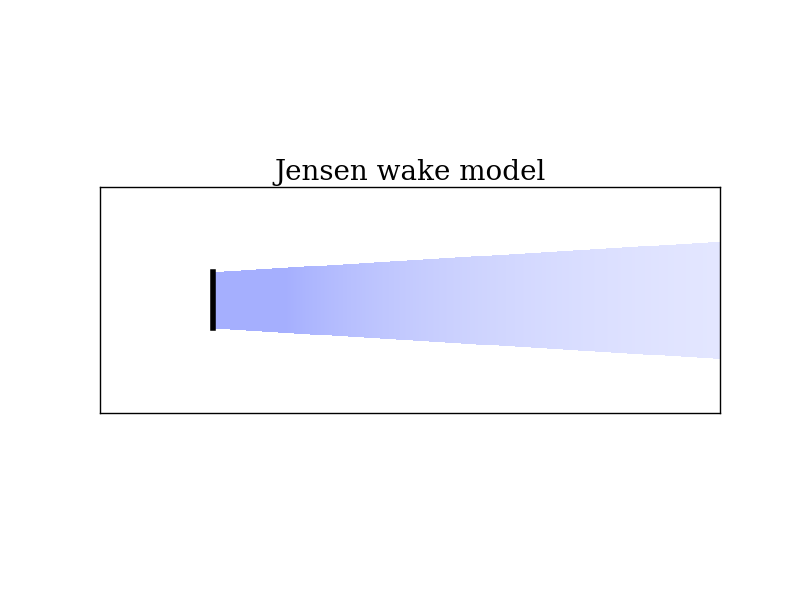
\includegraphics[trim={0 4cm 0 0}, clip,width=0.49\textwidth]{Figures/Jensen.png}\label{jensen}
   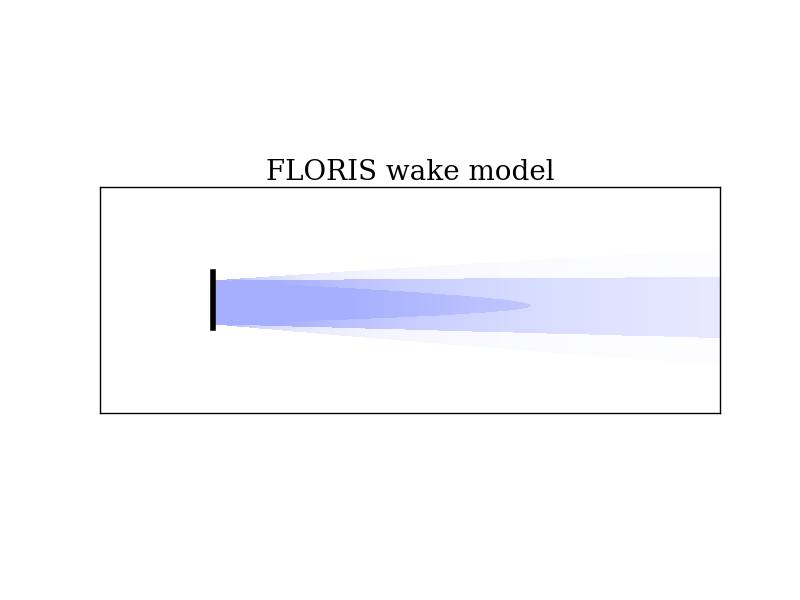
\includegraphics[trim={0 4cm 0 0}, clip,width=0.49\textwidth]{Figures/Floris.png}\label{floris}
  \caption{\label{wake_models} The Jensen and FLORIS wake models. Notice the three separate wake zones captured in the FLORIS wake model, and the single wake zone in the Jensen model.}
\end{figure}
The FLORIS model had some discontinuities in the original formulation. In this study we use a version that has been modified to be smooth and continuously differentiable, enabling gradient-based optimization \citep{thomas2017improving}.
%Check your citations for what type of style manual you are using (Chicago, APA, etc.) For most style manuals, all footnotes go at the end of the sentence.


The total wake deficit at any given point is defined as the square root of the sum of the squares of the loss contribution from each turbine wake:

\begin{equation}
L = \sqrt{\sum_{i=1}^\text{nTurbs}L_i^2}
\end{equation}

\noindent Thus at any point in the wind farm, the wind speed is:

\begin{equation}
V = V_\infty(1-L)
\end{equation}

\noindent Note that $V_\infty$ is defined as the freestream wind speed at the hub height of the wind turbine in question. Variations of the freestream wind speed are calculated with the wind profile power law: 
\begin{equation}
V = V_{\text{ref}}\Big(\frac{z}{z_{\text{ref}}}\Big)^\alpha
\label{Eq:shear}
\end{equation}
where $V_{\text{ref}}$ is the reference wind speed given by the wind data; $z_{\text{ref}}$ is height at which the reference wind speed was measured, which we assumed to be 50 meters; $V$ is the wind speed at and height $z$; and $\alpha$ is the wind shear exponent, which defines how the wind speed varies with height.
      
	\subsection{Annual Energy Production Calculation}
	\subsubsection{Power Calculation}
We assume that up to rated power, the rotation of each wind turbine can be controlled such that a constant power coefficient of 0.42 is achieved. The wind turbine power generation is defined as:

\begin{equation}
P = 
\begin{cases} 
      C_P\frac{1}{2}\rho V_{\text{eff}}^3A & V_{\text{eff}}\leq V_{\text{rated}} \\
      P_{\text{rated}} & V_{\text{eff}} > V_{\text{rated}}
   \end{cases}
\end{equation}

\noindent Where $C_P$ is the power coefficient, $\rho$ is the air density which we assumed was 1.1716 kg m$^{-3}$, $A$ is the swept area of the turbine rotor, and $V_{\text{eff}}$ is an effective wind speed across rotor, which is defined as:

\begin{equation}
V_{\text{eff}} = V(1-L)
\end{equation}

\noindent Where $V$ is the free stream wind speed at the turbine hub height, and L is the total velocity deficit.
%It is defined as an area-weighted average of the wind speeds across the rotor:
%Katie: Is it a weighted area? or is it a weighted average? If the area is weighted, then you need a hypen (area-weighted average). 

%\begin{equation}
%V_{\text{eff}} = \frac{\int_A V dA }{A}
%\end{equation}

%\noindent Again, in this equation, only the hub height velocities are considered. There is no vertical integration of the wind speed across the rotor hub. The wind shear is considered only in calculating the free stream wind speed.
%Katie:Why is this? Why not do vertical integration? Out of your scope? Ignore this if you talk about this earlier in the paper, as I've jumped to methodology. 


\subsubsection{Wind Direction and Speed Distributions}

We used two different empirical wind distributions; first we used wind data from the city of Alturas, California, second we used data from the Princess Amalia Wind Farm, off the coast of the Netherlands. 
%Katie: It almost seems as if this wind farm is both in the Netherlands and in California. You could either say. "from the city of Alturas, California and from the Princess Amalia Wind Farm, a wind farm off the coast of the Netherlands." OR "from both the Princess Amalia Wind Farm, a wind farm off the coast of the Netherlands, and the city of Alturas, California."
The data we have is separated into 36 bins every 10 degrees, and 72 bins every 5 degrees, respectively. Both wind roses are shown in Section \ref{sec:optimization}, Fig. \ref{wind_roses}.
%, and the Princess Amalia wind rose is shown in Figure \ref{amalia}. 

%\begin{figure}[htbp]
 % \centering
  %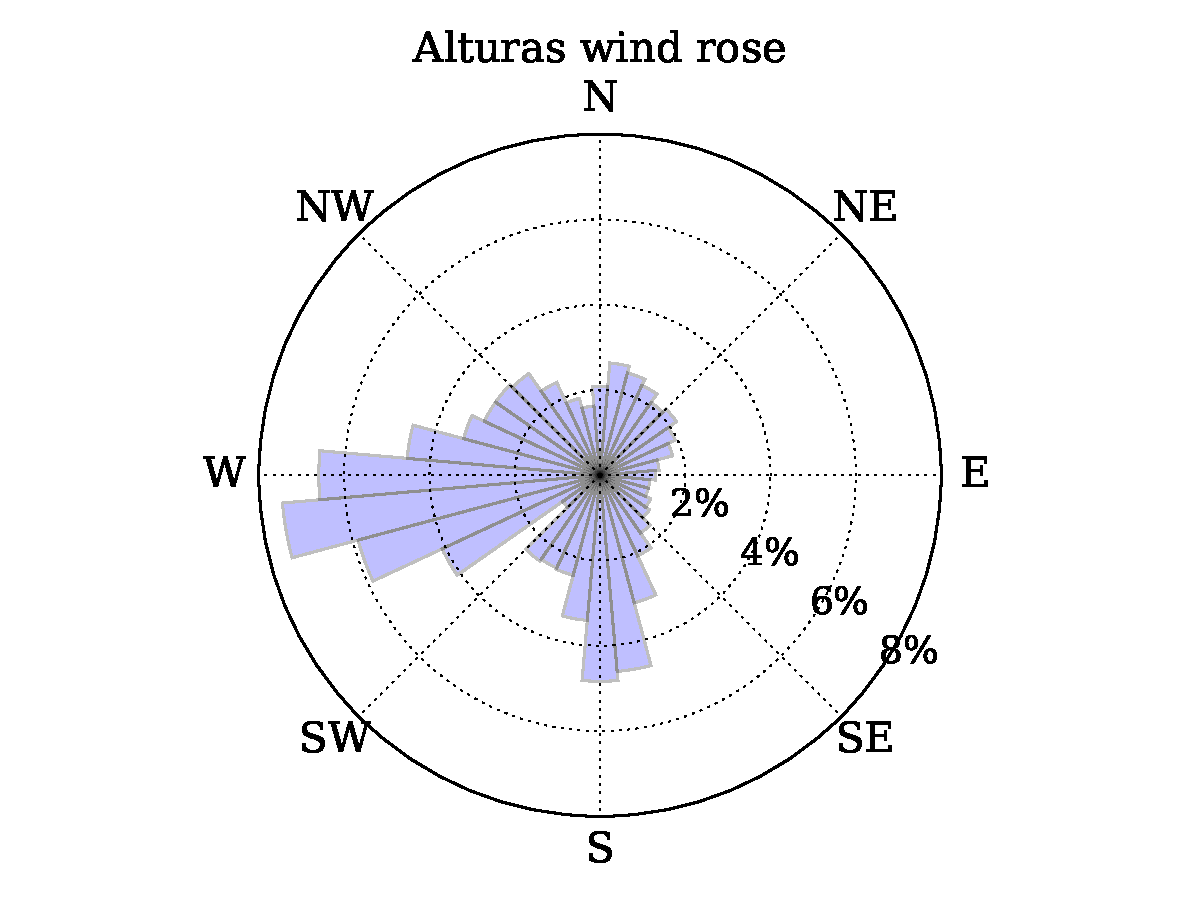
\includegraphics[width=0.49\textwidth]{Figures/alturas_rose.pdf}
  %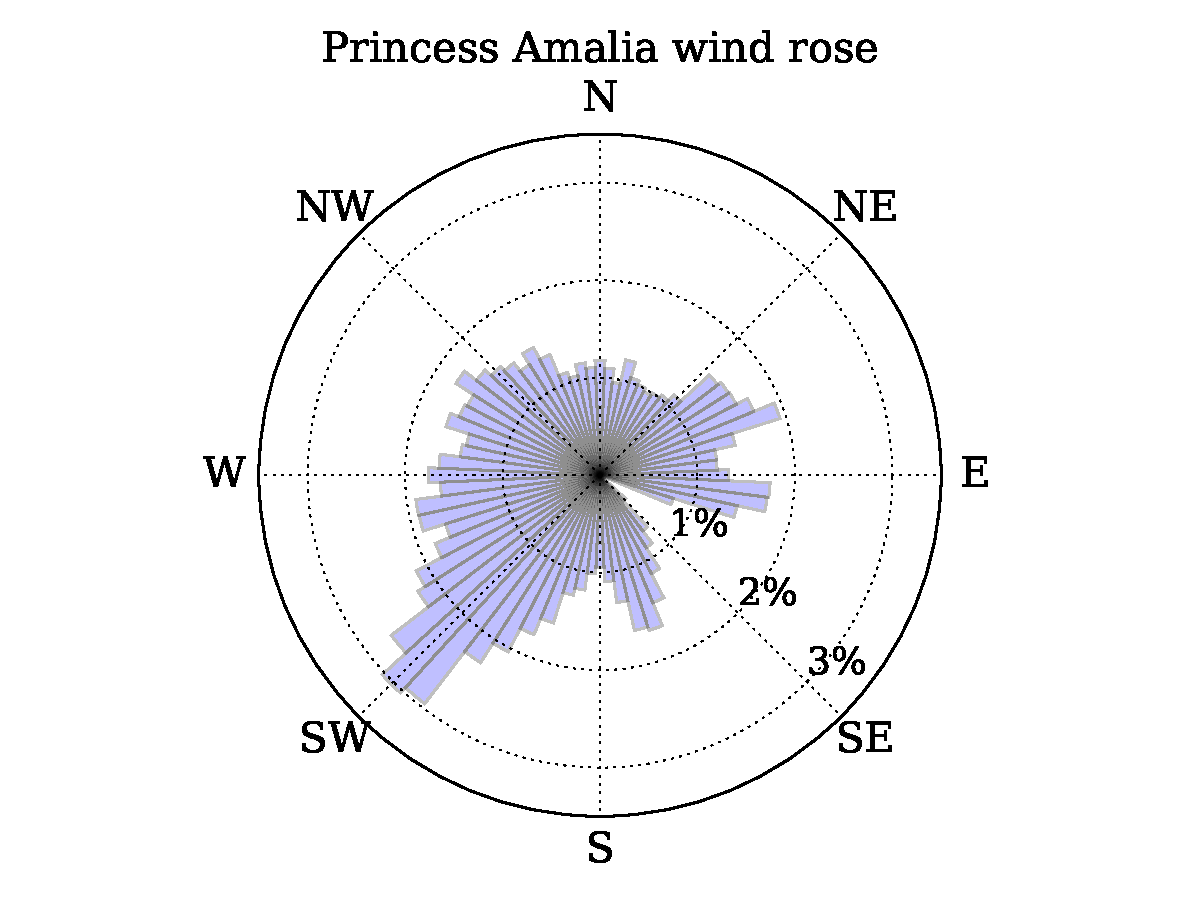
\includegraphics[width=0.49\textwidth]{Figures/amalia_rose.pdf}
  %\caption{\label{wind_roses} On the left, the wind direction distribution in Alturas, California, separated into 36 bins, every 10 degrees. On the right, the wind direction distribution of the Princess Amalia Wind Farm, separated into 72 bins, every 5 degrees.}
%\end{figure}

%\begin{figure}[htbp]
  %\centering
  %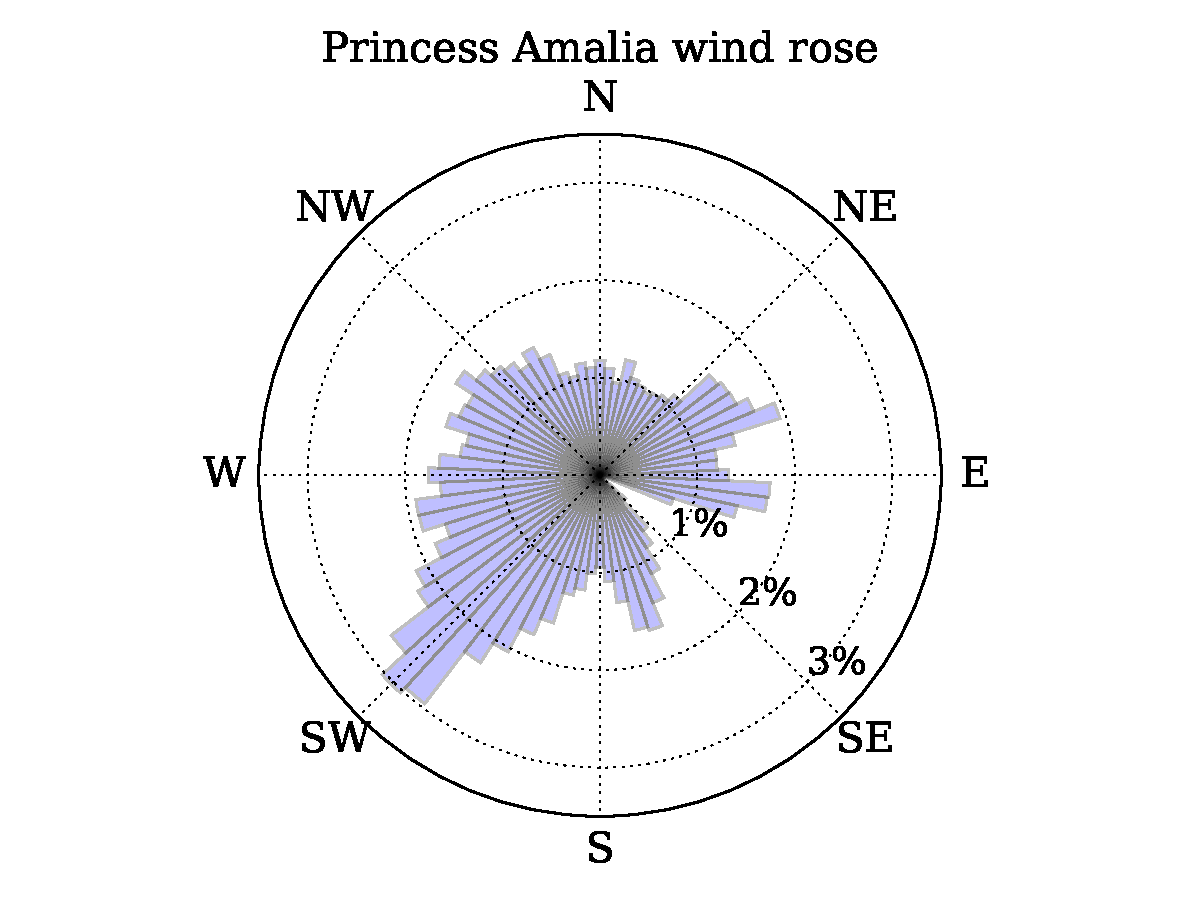
\includegraphics[width=0.75\textwidth]{Figures/amalia_rose.pdf}
  %\caption{\label{amalia} The wind direction distribution of the Princess Amalia Wind Farm, separated into 72 bins, every 5 degrees.}
%\end{figure}

%Just as wind direction varies, the wind speed at any direction also changes. 
We represented the speeds at any direction as a Weibull distribution, which is commonly used to represent wind speed distributions \citep{justus1978methods,rehman1994weibull,dorvlo2002estimating}: 
\begin{equation}
W(x) = \Big(\frac{k}{V_{\text{mean}}}\Big)\Big(\frac{x}{V_{\text{mean}}}\Big)^{k-1}\text{exp}\Big[\Big(-\frac{x}{V_{\text{mean}}}\Big)^k\Big]
\end{equation}
The shape factor, $k$, was set as 1.76. 
The mean speed for a given distribution, $V_{\text{mean}}$, can be different depending on the wind direction, meaning that each wind direction has an associated Weibull curve defining the wind speed distribution from that direction. The average speeds, $V_{\text{mean}}$, from every direction for each wind rose are shown in Section \ref{sec:optimization}, Fig. \ref{wind_speeds}.
%The average speed, $V_{\text{mean}}$, for each Weibull distribution is the average wind speed defined for every direction of each wind rose, meaning that each wind direction has an associated Weibull distribution defining the wind speeds from that direction. The average wind speeds from every direction for each wind rose are shown in Section \ref{sec:optimization}, Fig. \ref{wind_speeds}.
Figure \ref{weibull} shows the wind speed Weibull distributions for two different $V_{\text{mean}}$ values. 
%Because of a lack of reliable wind speed data for the Alturas wind rose, it is assumed to have an average wind speed of eight meters per second, which is uniform across all wind directions. For the Princess Amalia Wind Farm, $V_{\text{mean}}$ is defined as the directionally averaged wind speed for each wind direction (thus each direction has a different $V_{\text{mean}}$).
%for each wind direction is defined as the average wind speed from each wind direction. 
%These directionally averaged wind speeds are shown in Fig. \ref{amalia_speeds}. 

%\begin{figure}[htbp]
 % \centering
  %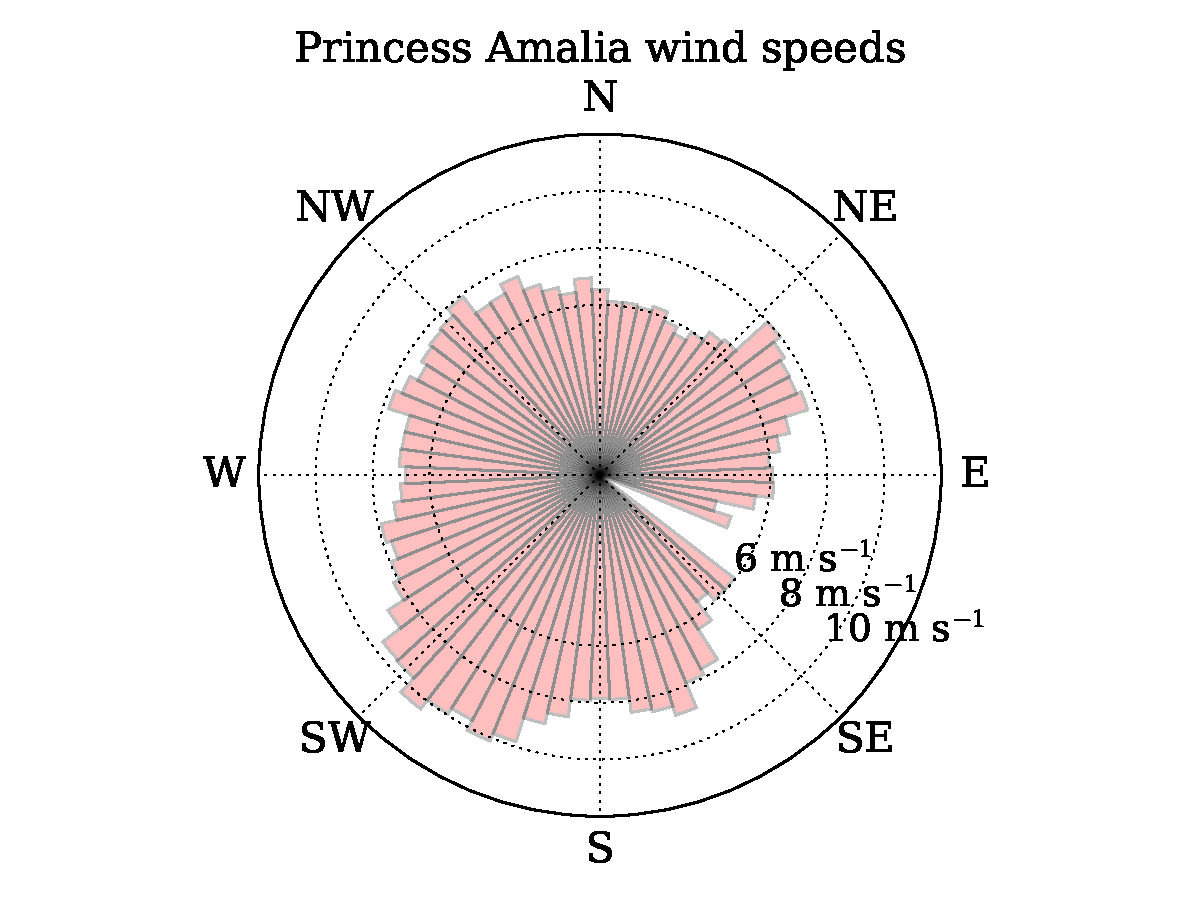
\includegraphics[width=0.49\textwidth]{Figures/amalia_speeds.pdf}
  %\caption{\label{amalia_speeds} The directionally averaged wind speeds of the Princess Amalia Wind Farm, separated into 72 bins, every 5 degrees.}
%\end{figure}
%Katie: Maybe this is obvious to people reading your paper, but why is the shape factor set at 1.76?

\begin{figure}[htbp]
  \centering
  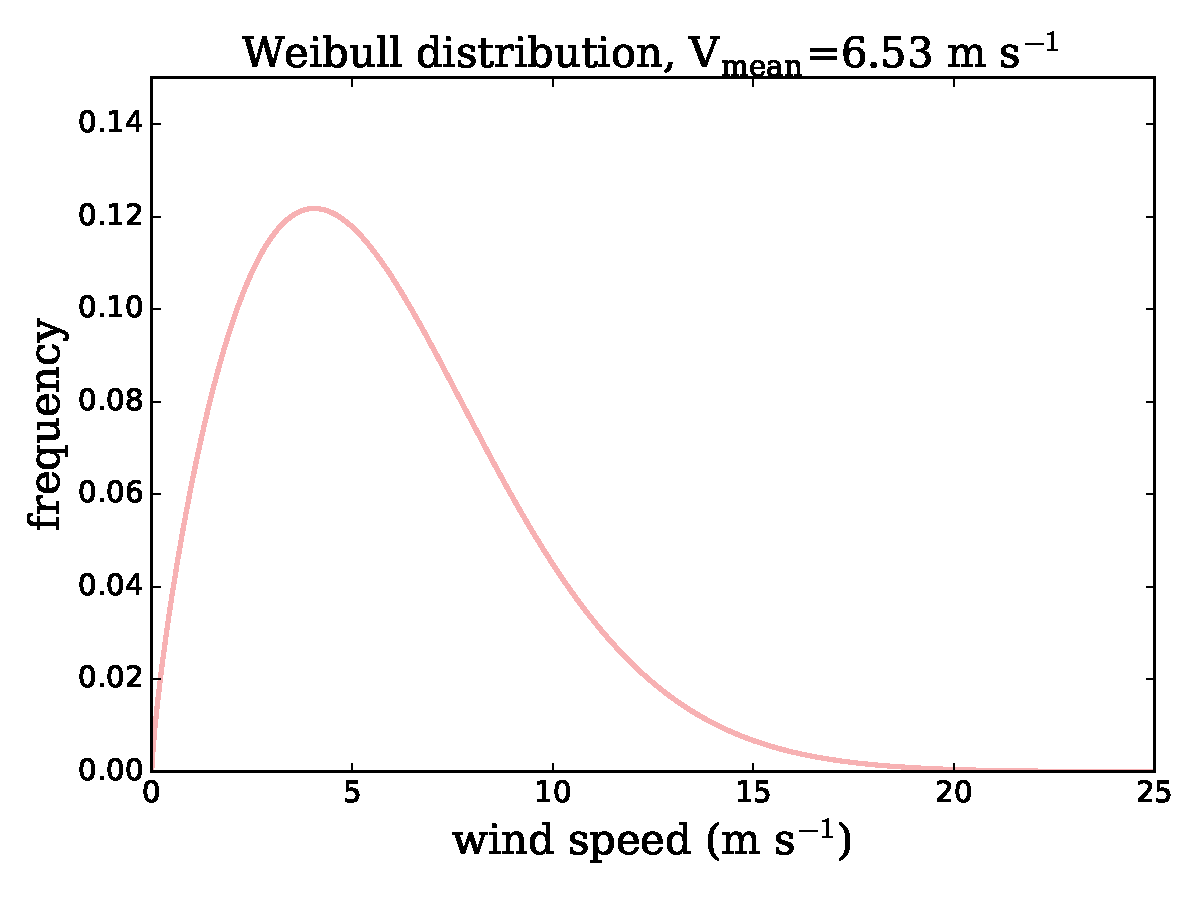
\includegraphics[width=0.4\textwidth]{Figures/weibull_6_53.pdf}\label{653}
  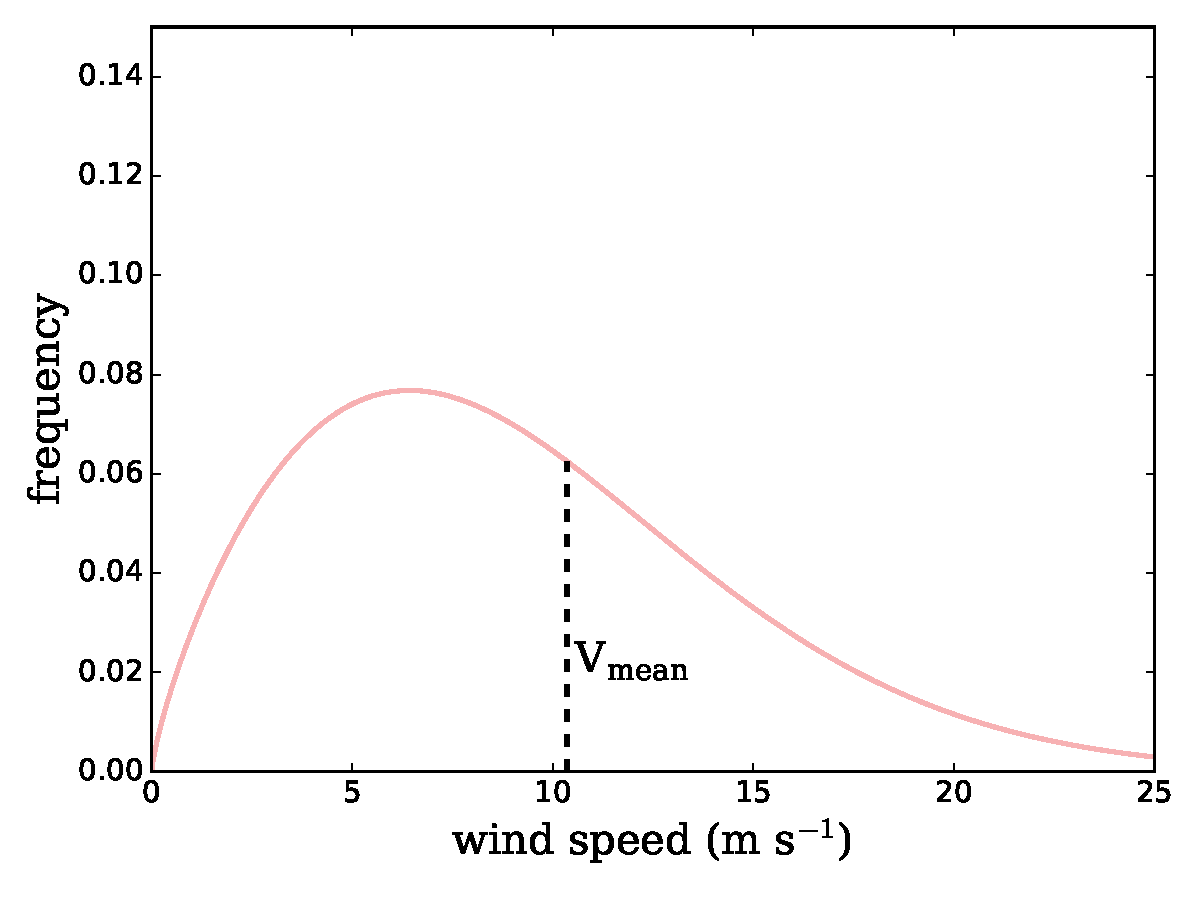
\includegraphics[width=0.4\textwidth]{Figures/weibull_10_35.pdf}\label{1035}
 % \subfloat[]{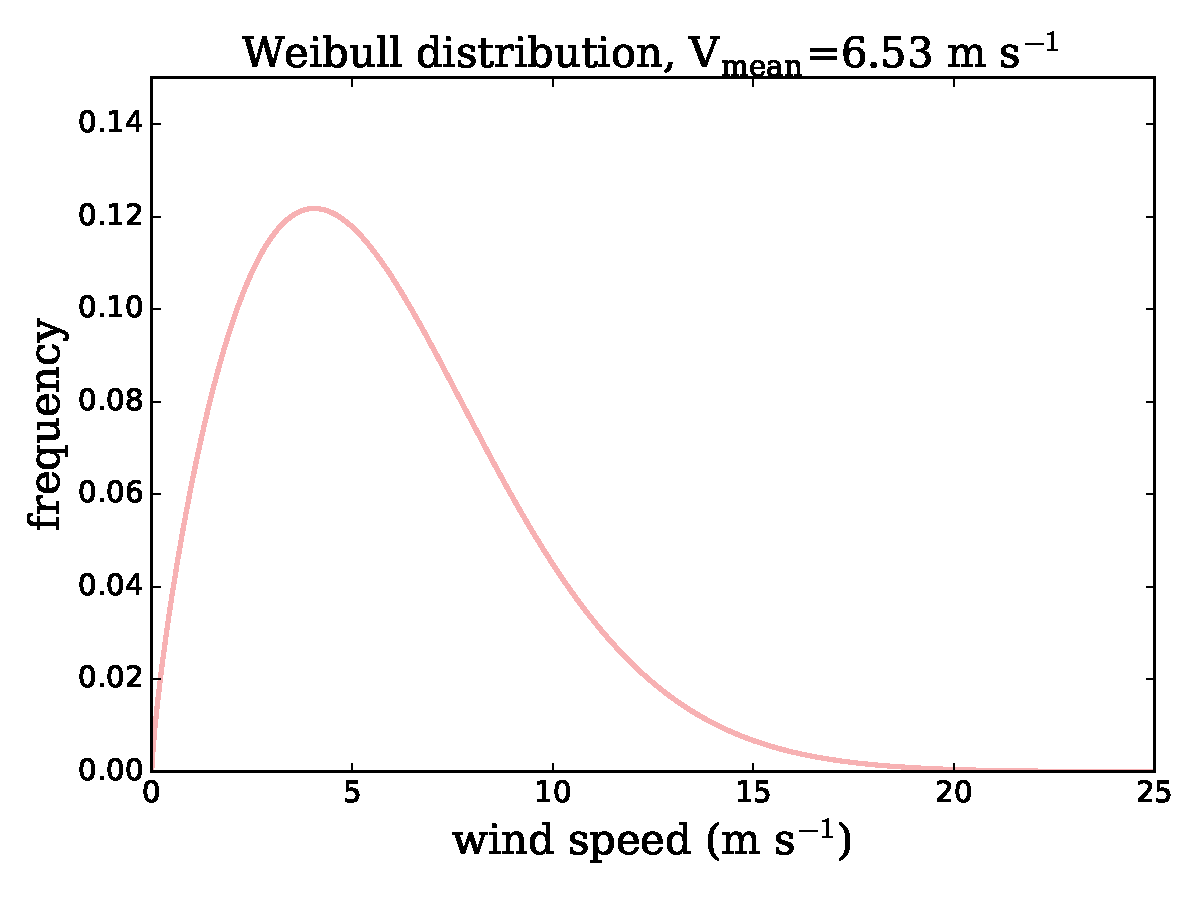
\includegraphics[width=0.5\textwidth]{Figures/weibull_6_53.pdf}\label{653}}
  %\subfloat[]{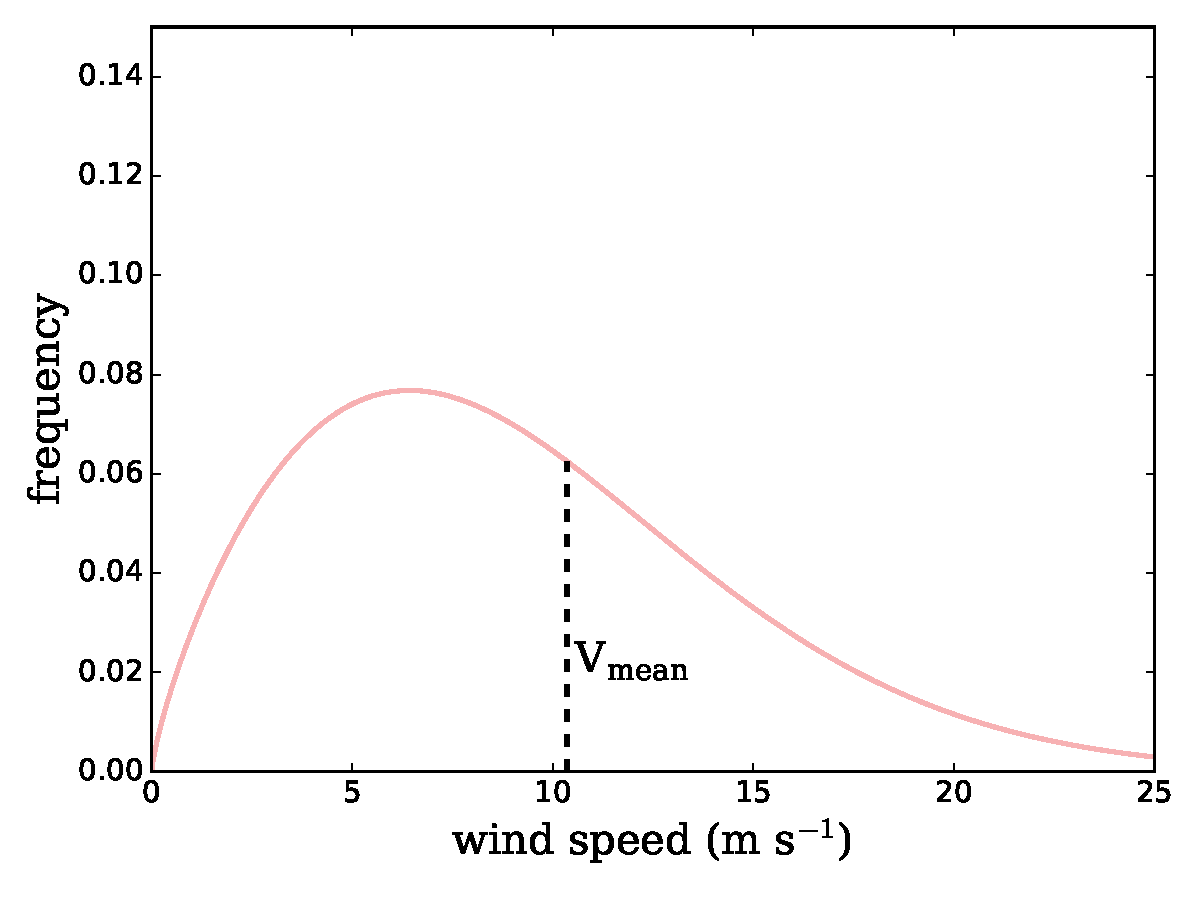
\includegraphics[width=0.5\textwidth]{Figures/weibull_10_35.pdf}\label{1035}}
  \caption{\label{weibull} The Weibull wind speed distributions for two different average wind speeds. In (a) there is an average wind speed of 6.53 meters per second, and (b) shows an average wind speed of 10.35 meters per second. The shape factor k in each Weibull distribution is chosen as 1.76.}
\end{figure}
%Katie: Why didn't you use a Weibull distribution for the California wind? Also you have misspelled distribution in Figure 5.



\subsubsection{Sampling}
The direction data we have is binned into 36 directions for one wind rose, and 72 directions for the other. This is very fine sampling, 
%Katie: Why spell out seventy two but leave 36? Is that part of your style guide? If not, choose one and remain consistent throughout the paper. 
more refined than necessary to accurately compute the annual energy production (AEP) of a wind farm. 
%Katie: Then why do fine sampling? Or are you saying that you didn't use all these bins? This part confused me a bit. 
For every wind direction at which the power is computed, the wake model must be called; therefore, reducing the number of directions at which the wind farm power is computed will reduce the time required to optimize. 
%Katie: Consider instead: Reducing the number of directions at which the wind farm power is computed will reduce the time required to optimize because  the wake model must be called for every wind direction at which the power is computed. 
However, too few directions and the AEP calculation will be inaccurate. We fit a spline to the direction data and were thus able to sample at any direction. We then performed a two-dimensional convergence study to find how many directions and speeds were required to approach the ``true'' AEP, which we defined to be the AEP calculated when using 50 wind directions and 30 wind speed samples. 
%Katie: The wording of the last sentence is odd and took me a while to figure it out. Also, you move between present tense and past tense in this entire methodologies section. Choose one. Also in the part "close to the true AEP" how close is close? Consider instead: We then performed a two dimensional convergence study to find how many directions and speeds were required to be almost equivalent to the ``true'' AEP. We found that 50 wind direction samples and 30 wind speed samples were necessary. However,
We found that at 23 wind direction samples and 5 wind speed samples from the Weibull distributions, the AEP converged within 2\% of the true AEP. This is within the error of our wake model; therefore, this number of samples was used in our study. 
%Katie: "this number of samples was used in our study, instead of the higher numbers that came slightly closer to true AEP. 

	\subsection{Tower Model}
	Because the tower height varied in this study, it was necessary to calculate the tower mass and perform structural analyses.
We modeled the tower as a tapered steel cylinder. As shown in Fig. \ref{tower_def}, the tower diameter and shell thickness were defined at the bottom, midpoint, and top of the tower, and were linearly interpolated in between.
The structural analysis was used to constrain the optimization, keeping the turbine towers from growing unrealistically tall, where failure from stress or buckling would be an issue. 
It was also necessary to provide gradients for all of our constraints, which included the von Mises stress, shell buckling, and global buckling at any point along the tower; the tower taper ratio; and the first natural frequency of the structure. A finite element model called TowerSE was developed at NREL that makes various calculations along the length of a tower \citep{ning2013towerse}. 
%Katie: Consider instead to make clearer and make the section flow smoothly (Get rid of last sentence and use this): To provide these gradients, we gathered necessary calculations from a a finite element model called TowerSE. Developed at NREL, TowerSE makes various calculations along the length of a tower. 
It is a powerful tool but does not provide analytic gradients. We optimized several wind farms using TowerSE and finite difference gradients, and consequently identified the shell buckling and first natural frequency as the only active constraints. We were then able to pull out the needed calculations from TowerSE and derive the associated gradients. 

\begin{figure}[htbp]
  \centering
  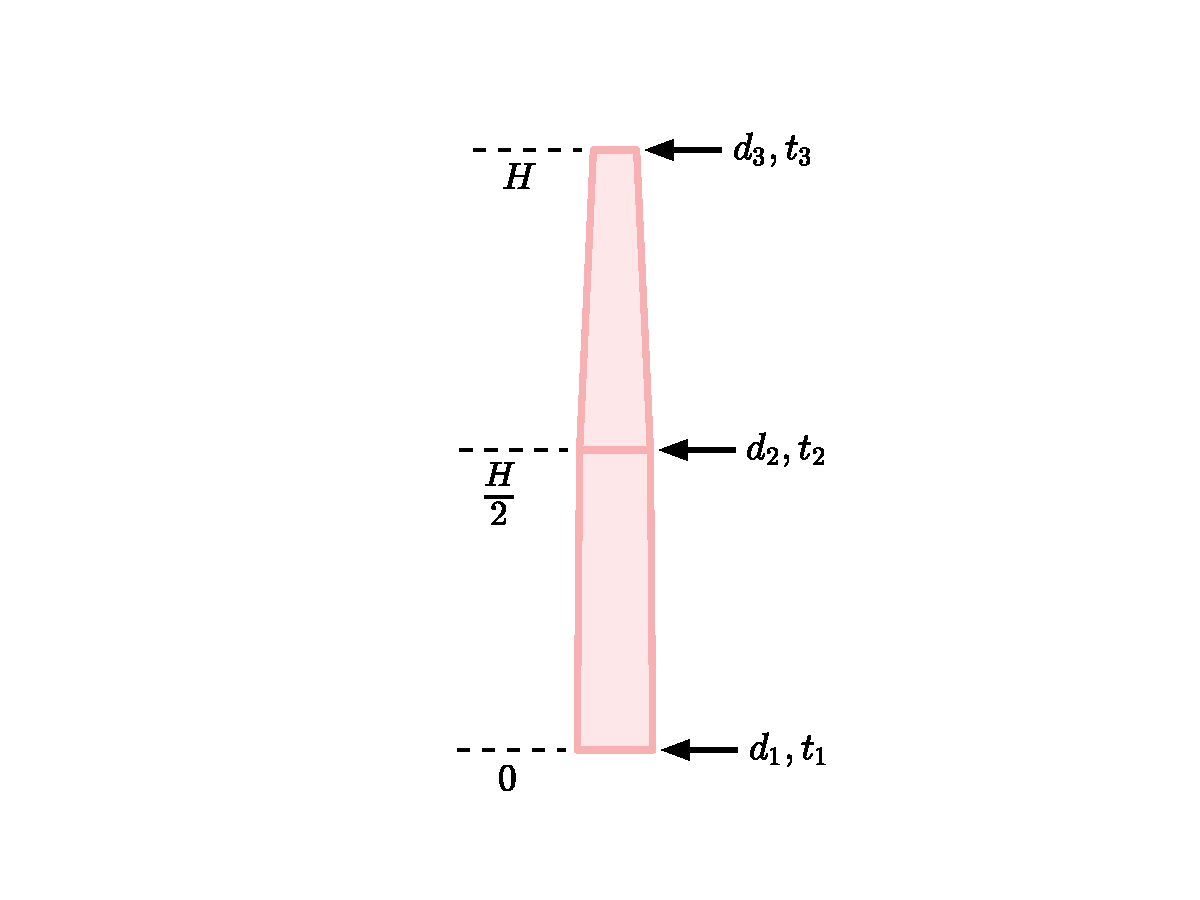
\includegraphics[width=0.7\textwidth]{Figures/tower_param.pdf}
  \caption{\label{tower_def} The parameterized turbine tower definition. The tower diameter and shell thickness are defined at the bottom, midpoint, and top of the tower, with the values linearly interpolated in between.}
\end{figure}

The tower mass was a simple calculation from the volume of the tower, the gradients solved by hand.
We calculated shell buckling as a function of the tower geometry and the stresses at each location, following the method outlined in Eurocode \citep{en19931}. These calculations were made in Fortran 90 for speed, and exact gradients were obtained with the Tapenade automatic differentiation tool \citep{hascoet2013tapenade}. We simplified the frequency calculation by approximating the tower as a cantilever beam of constant cross section with an end mass, and used the method described by Erturk et al.\ to calculate the natural frequency \citep{erturk2011appendix}. Because the turbine tower does not in reality 
%Katie: "does not really" sounds casual
have a constant mass density along the length and the mass from the rotor nacelle assembly is slightly offset at the top, our calculation is slightly more conservative than that predicted by TowerSE by about 10\%. 
%Consider instead for flow and clarity: is slightly more conservative than that predicted by TowerSE, about 10\% more conservative 
%more conservative could be replaced by lower frequency or higher frequency depending on what conservative means in this case. 
For this reason we scaled our frequency calculation by 10\% to more closely match the frequency calculated by TowerSE. We chose this simplified model so that we could find gradients, which were obtained using analytic sensitivity equations. 

	\subsection{Rotor/Nacelle Models}
	\label{rotor_nacelle}

The variable rotor diameter, turbine power rating, and blade and chord distributions in this study also must be accounted for in structural analysis.  To do so, we used another model developed at NREL called RotorSE \citep{ning2013rotorse} to calculate the rotor mass, rated and extreme thrust, rated torque, rated wind speed, and moments of inertia. The complex nature of RotorSE allows the user to fully define a rotor and perform analysis, however this comes at a cost in computation time. Because we coupled turbine design and turbine layout optimization, the rotor analysis needed to be called many more times than in an isolated turbine design optimization. 
Thus, to speed up the rotor calculations in our optimization, we created a surrogate model on the results provided by RotorSE. We sampled rotor diameters evenly spaced from 46 meters to 160 meters, every six meters, and rated powers from 0.5 megawatts to ten megawatts, every 0.5 megawatts. The lower limits, 46 meter rotor diameter and 500 kilowatt rated power, are both lower than we expected any of the optimal values to be. The upper limits, 160 meter rotor diameter and 10 megawatt rated power are both near the upper limit of current wind turbine technology. For each combination of rotor diameter and rated power, we used RotorSE to minimize the blade mass using the blade chord and twist distributions as design variables. The optimization was constrained such that the turbine blades would not fail from stress or buckling, and the power coefficient was greater than 0.42. Note that we did not vary the airfoils in the optimizations. 
%
We then used the converged optimizations, and used k-fold cross-validation with 10 groups to choose a fifth order bivariate spline which was then applied to each of the outputs of interest. This spline function was then used in place of RotorSE in our wind farm optimizations. By creating the surrogate, we achieved the accuracy of RotorSE without the large associated time requirement, as well as fast and simple analytic gradients. 
The k-fold cross-validation with 10 groups showed that the mean error is below 4\% for the moments of inertia, approximately 4.5\% for the extreme thrust, and below 3\% for the rest of the fits. 
Figure \ref{rotor_nacelle} shows the normalized surface fits for each of the variables of interest.


\begin{figure}[htbp]
  \centering
  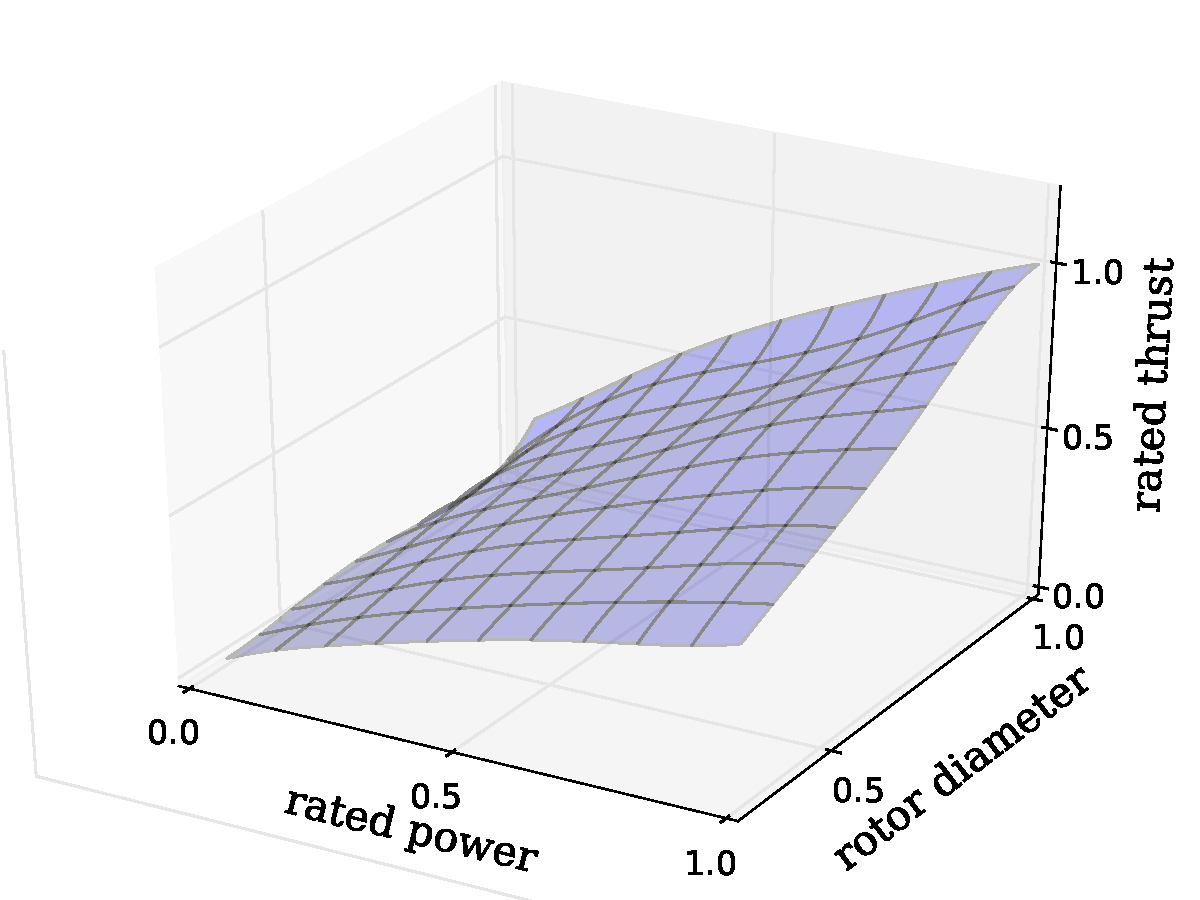
\includegraphics[trim={2cm 0 0 0},clip,width=0.33\textwidth]{Figures/rated_thrust.pdf}\label{rated_thrust}
  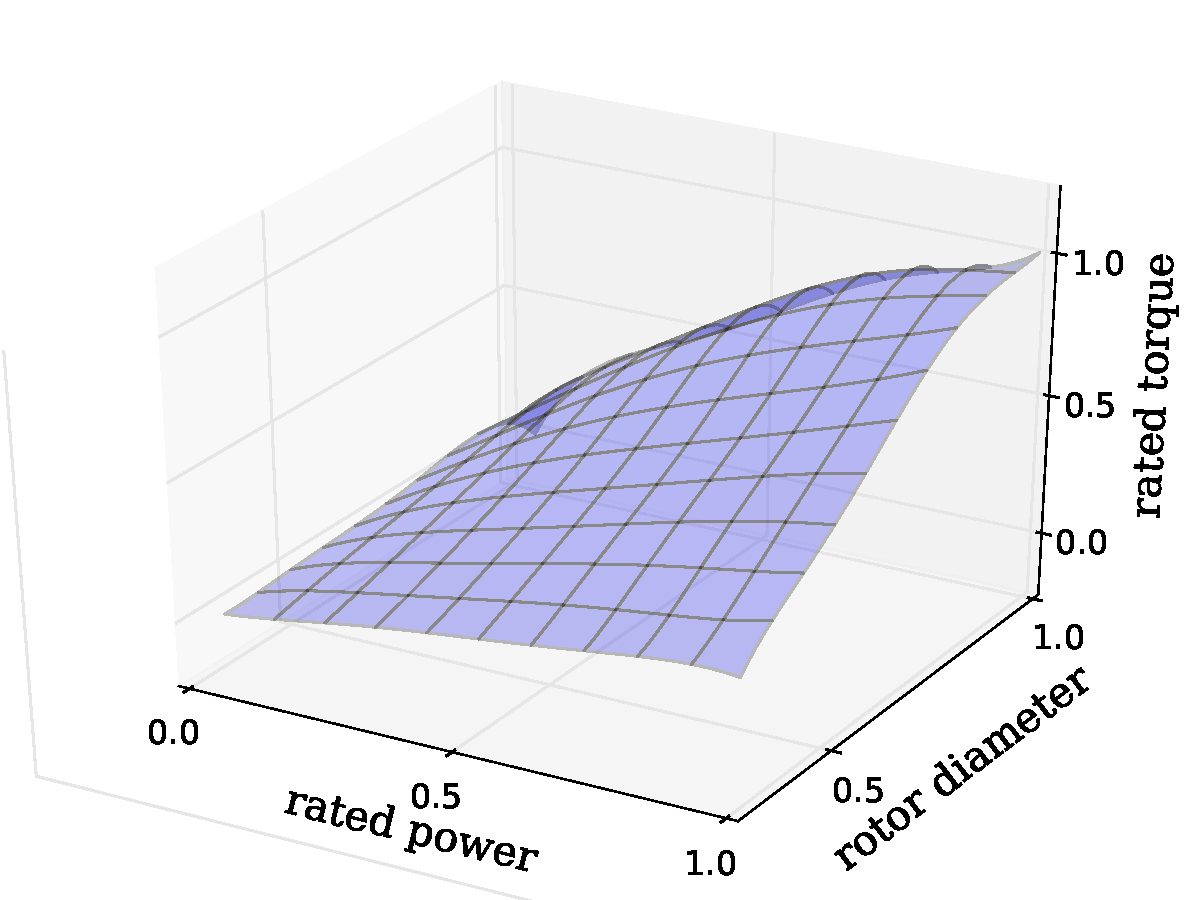
\includegraphics[trim={2cm 0 0 0},clip,width=0.33\textwidth]{Figures/rated_torque.pdf}\label{rated_torque}
 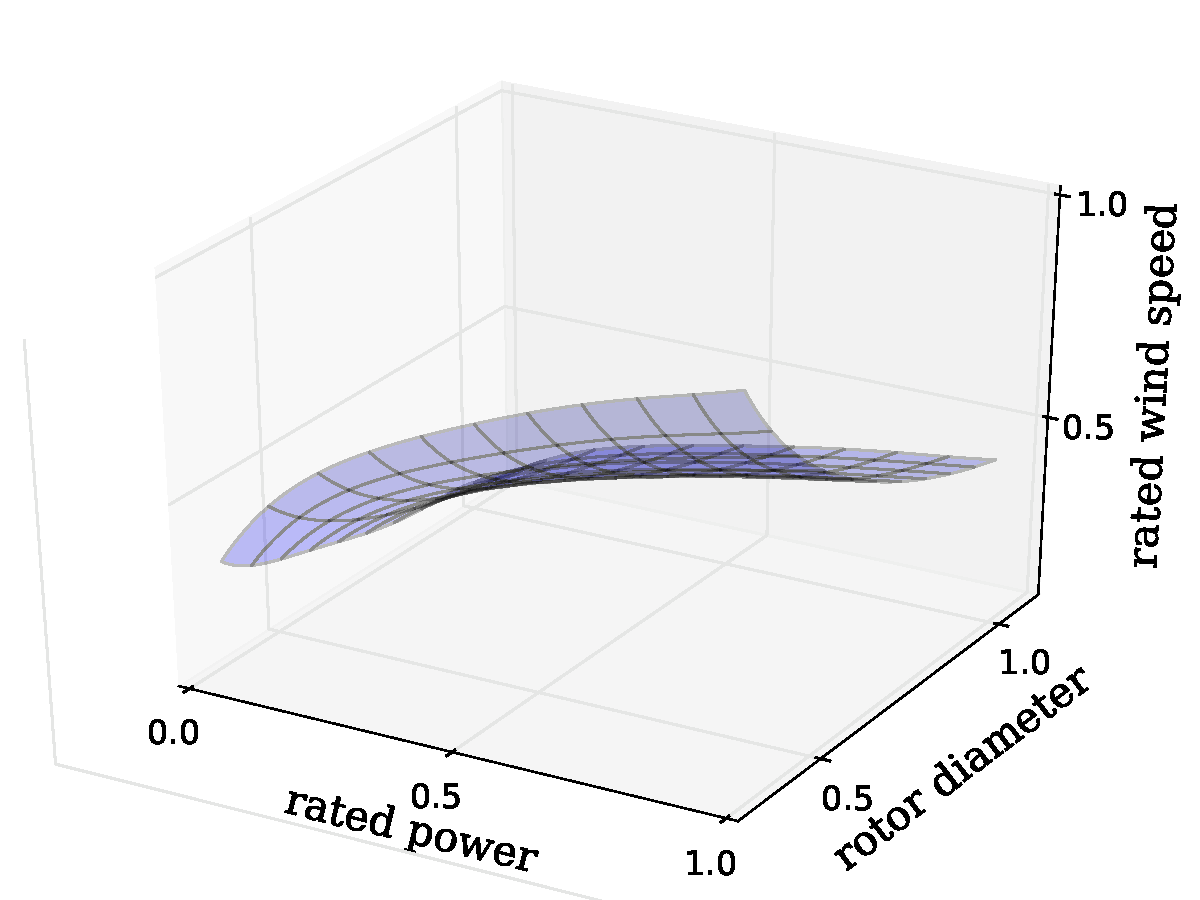
\includegraphics[trim={2cm 0 0 0},clip,width=0.33\textwidth]{Figures/rated_wind_speed.pdf}\label{rated_wind_speed}\\
  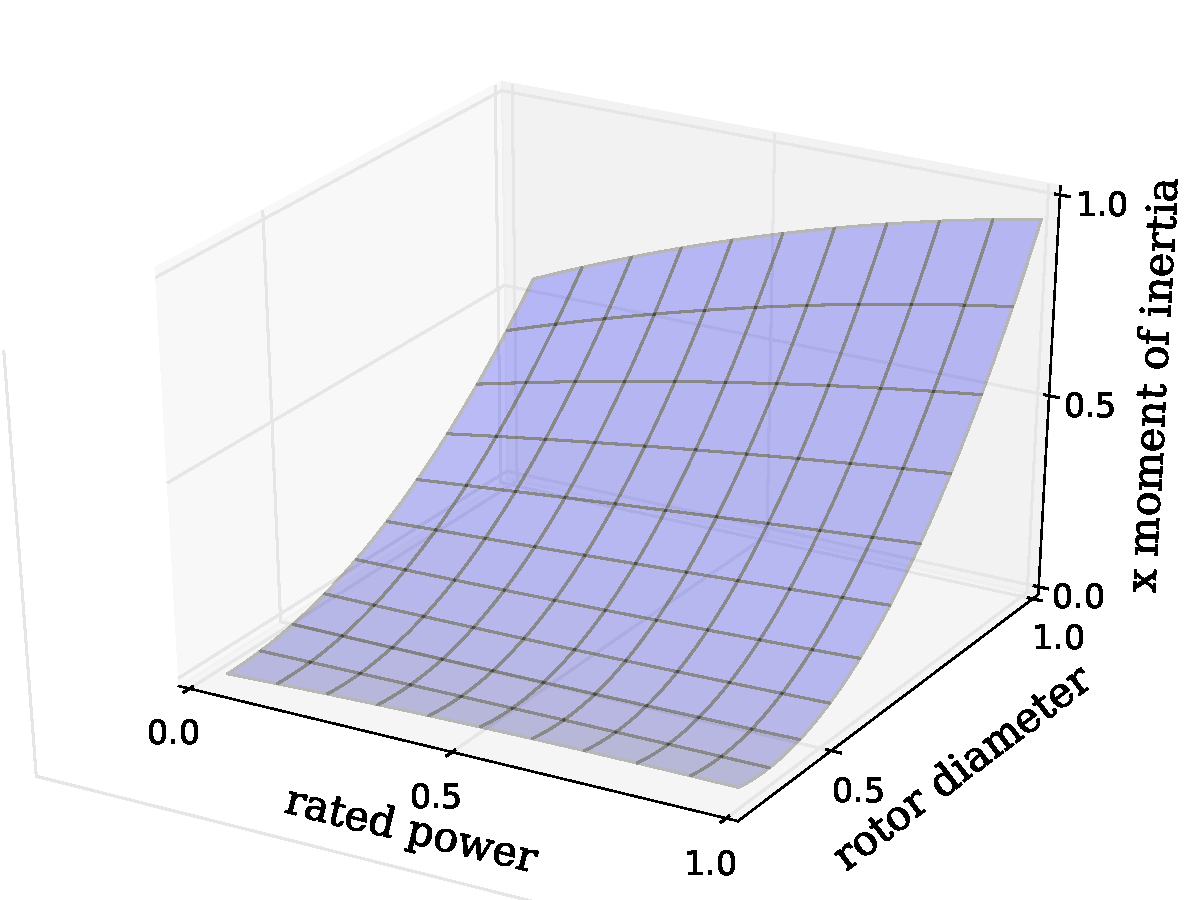
\includegraphics[trim={2cm 0 0 0},clip,width=0.33\textwidth]{Figures/x_mom_inertia.pdf}\label{xI}
  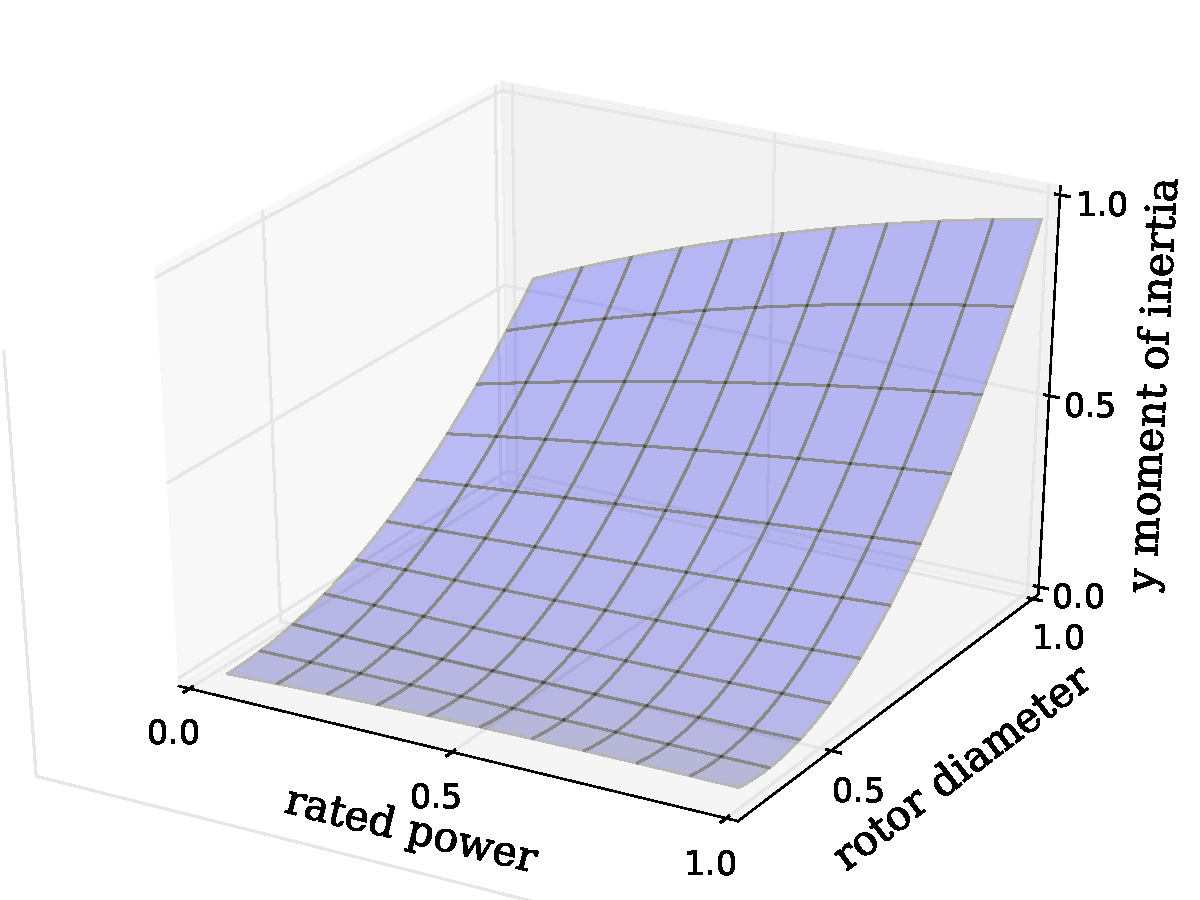
\includegraphics[trim={2cm 0 0 0},clip,width=0.33\textwidth]{Figures/y_mom_inertia.pdf}\label{yI}
  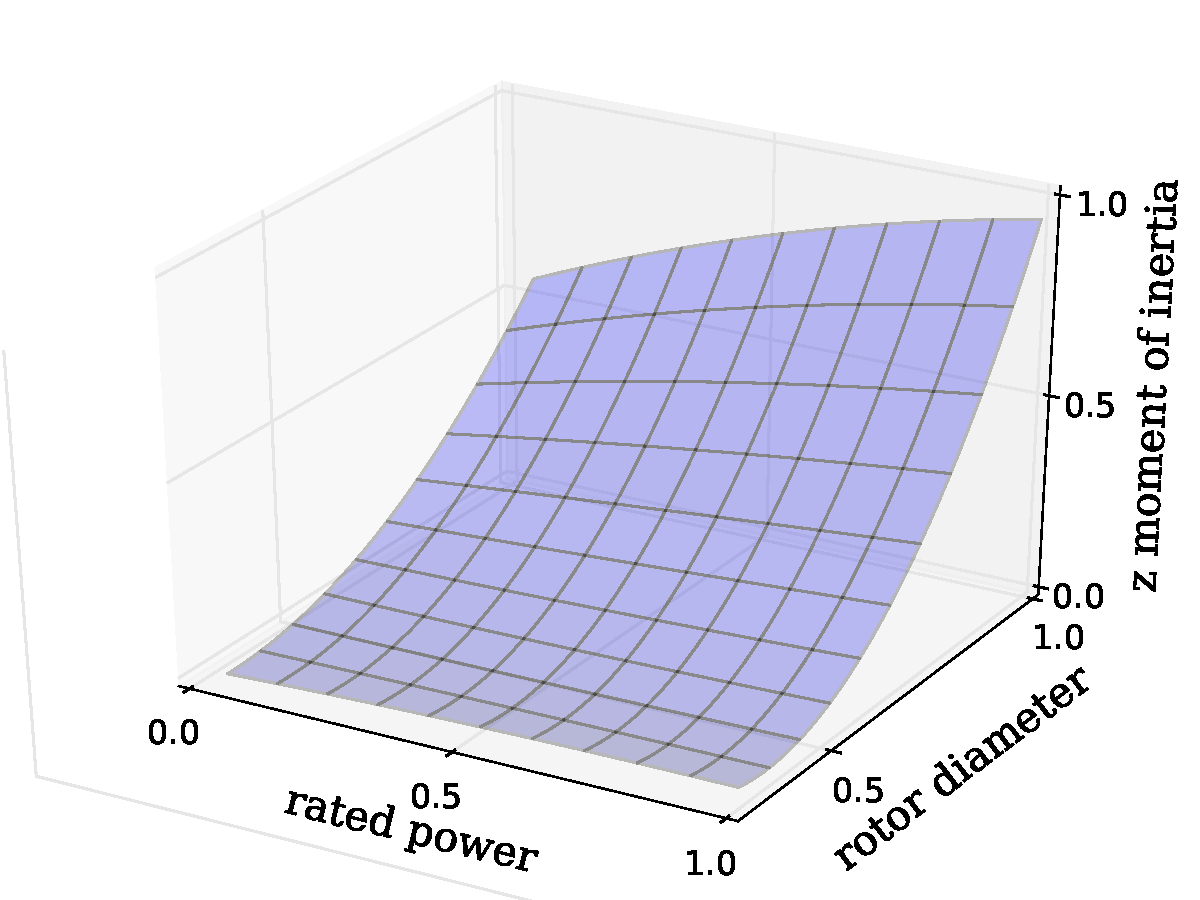
\includegraphics[trim={2cm 0 0 0},clip,width=0.33\textwidth]{Figures/z_mom_inertia.pdf}\label{zI} \\
 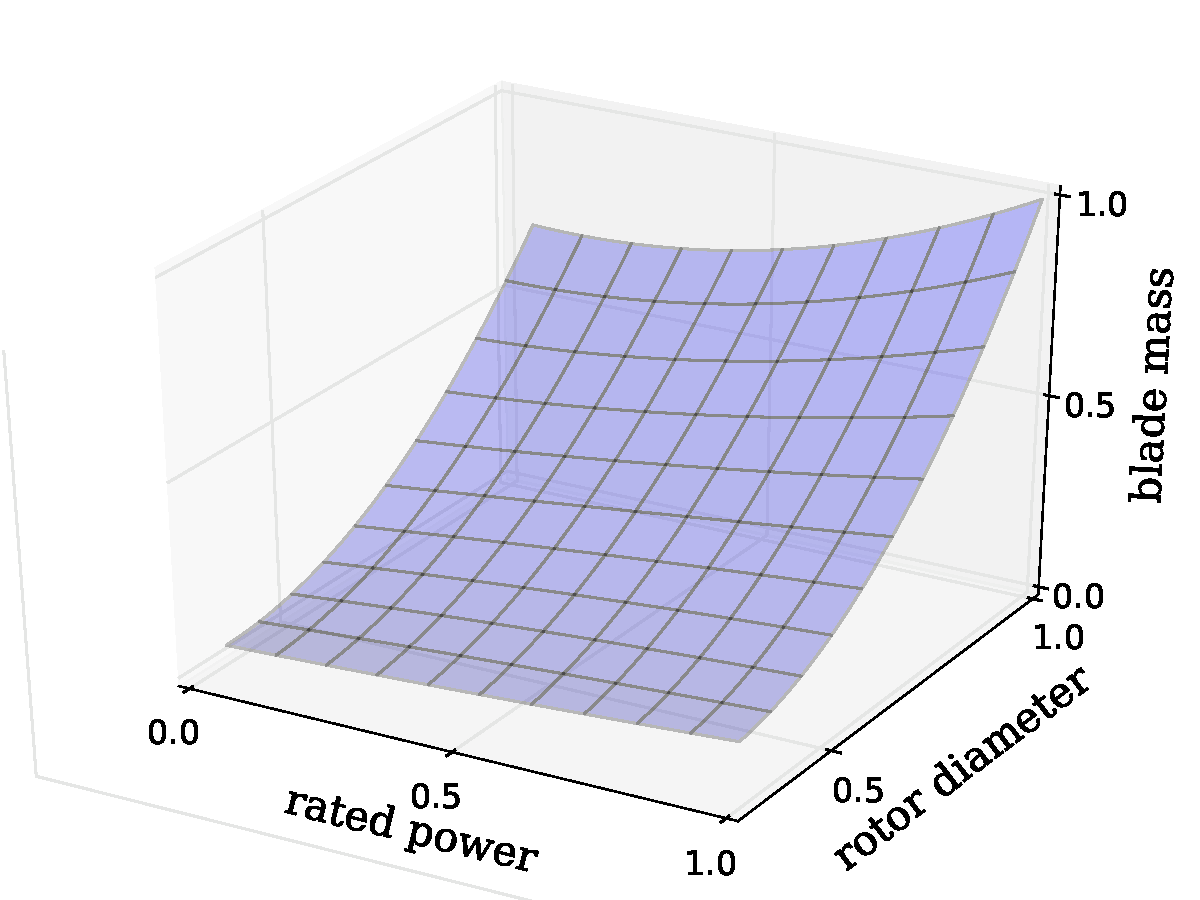
\includegraphics[trim={2cm 0 0 0},clip,width=0.33\textwidth]{Figures/blade_mass.pdf}\label{blade_mass}
 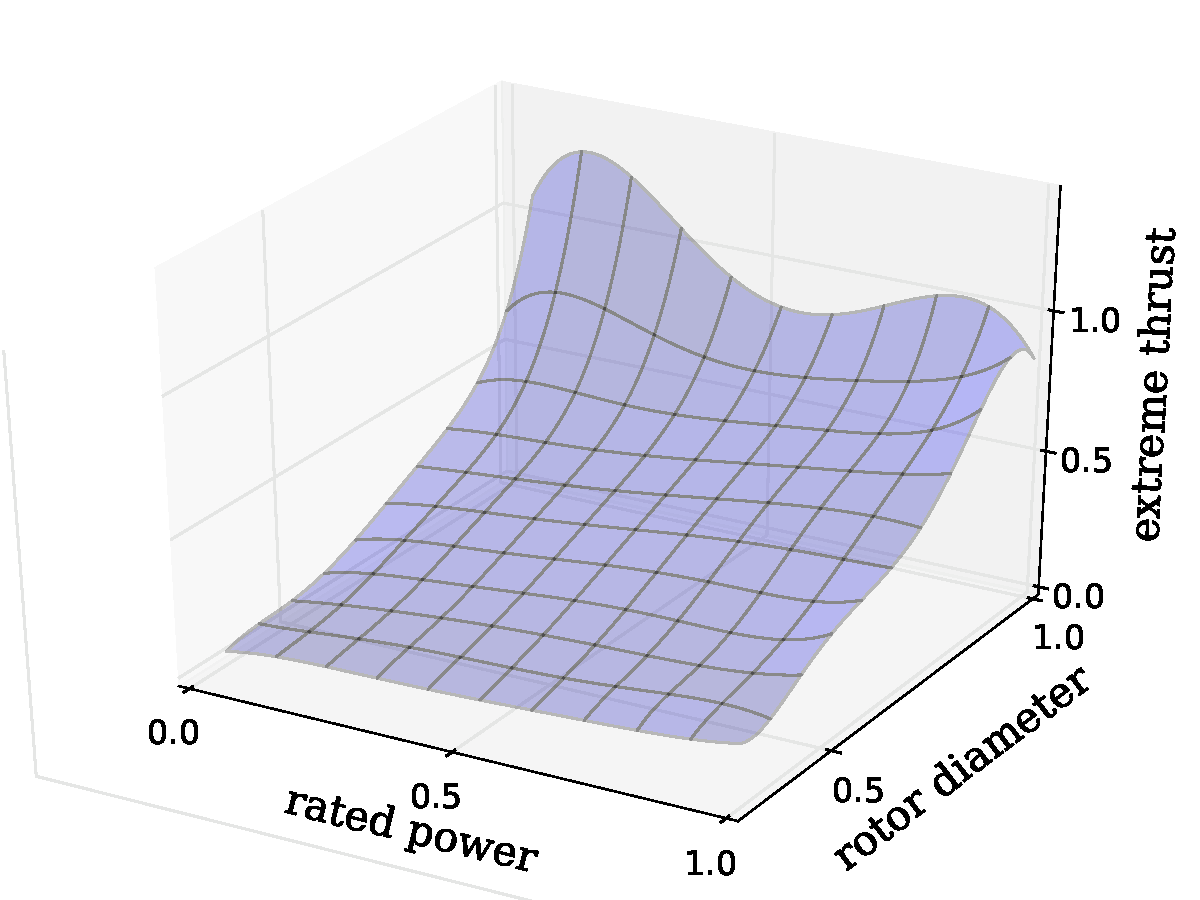
\includegraphics[trim={2cm 0 0 0},clip,width=0.33\textwidth]{Figures/extreme_thrust.pdf}\label{extreme_thrust}
  \caption{\label{rotor_nacelle} The spline fits to optimized RotorSE data. These fits were used to obtain the desired parameters of rotor mass, rated and extreme thrust, rated torque, rated wind speed, and moments of inertia as functions of the rotor diameter and rated power.}
\end{figure}

	\subsection{Cost Model}
	

AEP is a standard objective in wind farm optimization problems because it is easy to calculate and is a valid measure when only power production is affected by the optimization. When aspects of turbine design are included as design variables, this measure is no longer appropriate because of costs of the wind farm are effected as well. To accurately represent the trade-offs between power production and cost, we evaluated our wind farm by its COE as was done in our previous paper on wind farms with different turbine heights \citep{stanley2018}.              

	\subsection{Optimization}
	\label{sec:optimization}
	We set up our optimization with two different turbine groups. We assigned each turbine to one of two groups, where all turbines in a group had the same tower hub height, rotor diameter, turbine rating, tower diameter, tower shell thickness, and blade chord and twist distributions.
Rather than optimize each turbine, we chose two groups because our previous study in which we optimized wind farms with different turbine heights indicated that the most benefit comes from increasing from one height group to two. Any benefit from introducing more groups was marginal \citep{stanley2018}. We parameterized the tower by specifying the diameter and shell thickness at the bottom, midpoint, and top of the tower and then linearly interpolating diameter and shell thickness at points in between, as shown in Fig. \ref{tower_def}.

\begin{figure}[htbp]
  \centering
  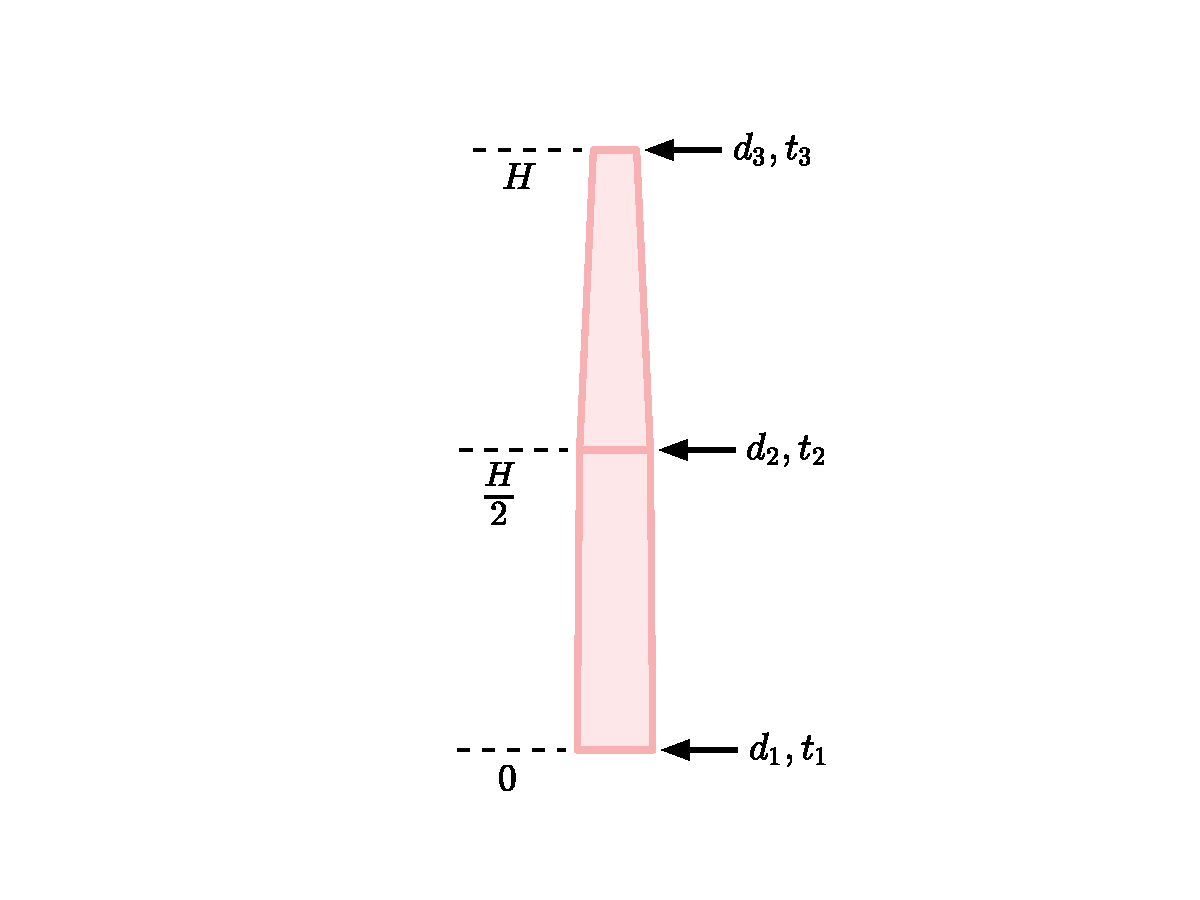
\includegraphics[width=0.5\textwidth]{Figures/tower_param.pdf}
  \caption{\label{tower_def} The parameterized turbine tower definition. The tower diameter and shell thickness are defined at the bottom, midpoint, and top of the tower, with the values linearly interpolated in between.}
\end{figure}
        
        It may be beneficial to do a binary optimization in which each turbine can change the turbine group to which it belongs, but this greatly increases the complexity of the optimization and makes it gradient-free. Gradient-free optimization is more computationally expensive, which severely limits the number of design variables we can include in the problem. To maintain the gradient-based optimization, we assigned each turbine to one of the groups before starting the optimization. Although the turbines can move throughout the wind farm, once assigned a turbine could not switch to the other group. In this study, we only examine an equal weighting of turbines in each group, but additional benefit may come from optimally choosing the number of turbines in each group.
        
        We ran several cases in which different design variables were included in the problem to allow comparison of their effects on COE. In all, the design variables we included were the position of each turbine ($x_i,y_i$), the tower height of each group ($H_1, H_2$), the rotor diameter of each group ($D_1, D_2$), the rated power of each group ($R_1, R_2$), the tower diameter of each group ($d_{1,j}, d_{2,j}$), and the tower shell thickness of each group ($t_{1,j}, t_{2,j}$). Index j refers location on the tower (j=1 is at the bottom, j=2 at the midpoint, j=3 at the top), meaning there are six total variables to define diameter (three for each height group), and six to define the tower shell thickness.
                
          The turbine layout and structural constraints were previously formulated in our multiple-hub-height study \citep{stanley2018}. Because rotor diameter was a design variable, the turbine spacing constraint was slightly reformulated such that the distance between any two turbines in the wind farm was greater than the sum of the two rotor diameters.
           The rotor diameter and the turbine rating were constrained by the lowest and highest values that were included in the RotorSE optimization, as discussed in Sect. \ref{rotor_nacelle}.
           The lower limits were never active in these optimizations, however some of the upper limits were active as will be seen in the Results section.
       The optimization can be expressed:
        
        
        \begin{equation}
			\begin{aligned}
				& \text{minimize}
					& & \text{COE} \\
                & \text{w.r.t.} 
                	&& x_i,~ y_i,~ H_{1,2},~ D_{1,2},~ R_{1,2},~ d_{(1,j)},~ d_{(2,j)},~ t_{(1,j)},~t_{(2,j)}\\
                		&&& i = 1, \ldots, n; \; j = 1,~2,~3 \\
				& \text{subject to}
					& & \text{boundary constraints} \\
						&&& \sqrt{(x-x_i)^2+(y-y_i)^2} \geq 2D_{\text{rotor}} \\
						&&& H_1-\frac{D_1}{2}, H_2-\frac{D_2}{2} \geq 10~ \text{m}\\
                		&&& d_{(1,j),(2,j)} \leq 6.3~ \text{m}\\
                		&&& d_{(1,top),(2,top)} \geq 3.87~ \text{m}\\
						&&& \frac{3\hspace{0.08cm}\Omega}{1.1} \geq f_{1,2} \geq 1.1\hspace{0.08cm}\Omega \\
                		&&& \text{shell buckling margins: max thrust} \leq 1 \\
                        &&& \text{shell buckling margins: survival load} \leq 1 \\
                		&&& \frac{d_{(1,j)}}{t_{(1,j)}},\frac{d_{(2,j)}}{t_{(2,j)}} \geq 120\\
                        &&& 46~ \text{m} < D_1,D_2 < 160~ \text{m}  \\
                        &&& 500~ \text{kW} < R_1,R_2 < 10,000~ \text{kW} \\
			\end{aligned}
		\end{equation}
%
Note that i is the index defining the wind turbine, and j is the index describing the location on the tower.
        
        The gradients for this optimization were all analytic. We calculated the partial derivatives of each small section of the model and included each part in a framework called OpenMDAO, which calculates the gradients of the entire system \citep{gray2010openmdao}. The analytic gradients are significant because they are more accurate, converge to better solutions, and converge on the solution much faster that finite difference gradients. More importantly, they allow us to solve much larger optimization problems. 
        
We optimized two different wind farms, each with several different wind shear exponents and turbine spacing multipliers as will be explained later in this section. 
The first wind farm is a fictional 32-turbine wind farm with a circular boundary, shown in Fig. \ref{layouts}.
This wind farm was optimized with wind data from the city of Alturas, California, shown in Fig. \ref{wind_roses}. For lack of reliable data, the average wind speed, $V_{\text{mean}}$, from each direction of this wind rose was assumed to be eight meters per second, shown in Fig \ref{wind_speeds}.
The second wind farm is the Princess Amalia wind farm, a real farm off the coast of the Netherlands which has 60 wind turbines, is shown in Fig. \ref{layouts}. This wind farm was optimized with the wind direction and average directional speed data from the true Princess Amalia farm, shown in Figs. \ref{wind_roses} and \ref{wind_speeds}. The farm boundary for the Princess Amalia wind farm is the convex hull of the original Princess Amalia layout. The baseline turbine layout and boundaries are shown in Fig. \ref{layouts}. The turbines in both wind farms are Vestas 2 Megawatt wind turbines, which have a rotor diameter of 80 meters. Therefore, we used a baseline rotor diameter of 80 meters and a baseline power rating of 2 Megawatts. The baseline hub height used in this study was 100 meters. 

\begin{figure}[htbp]
  \centering
   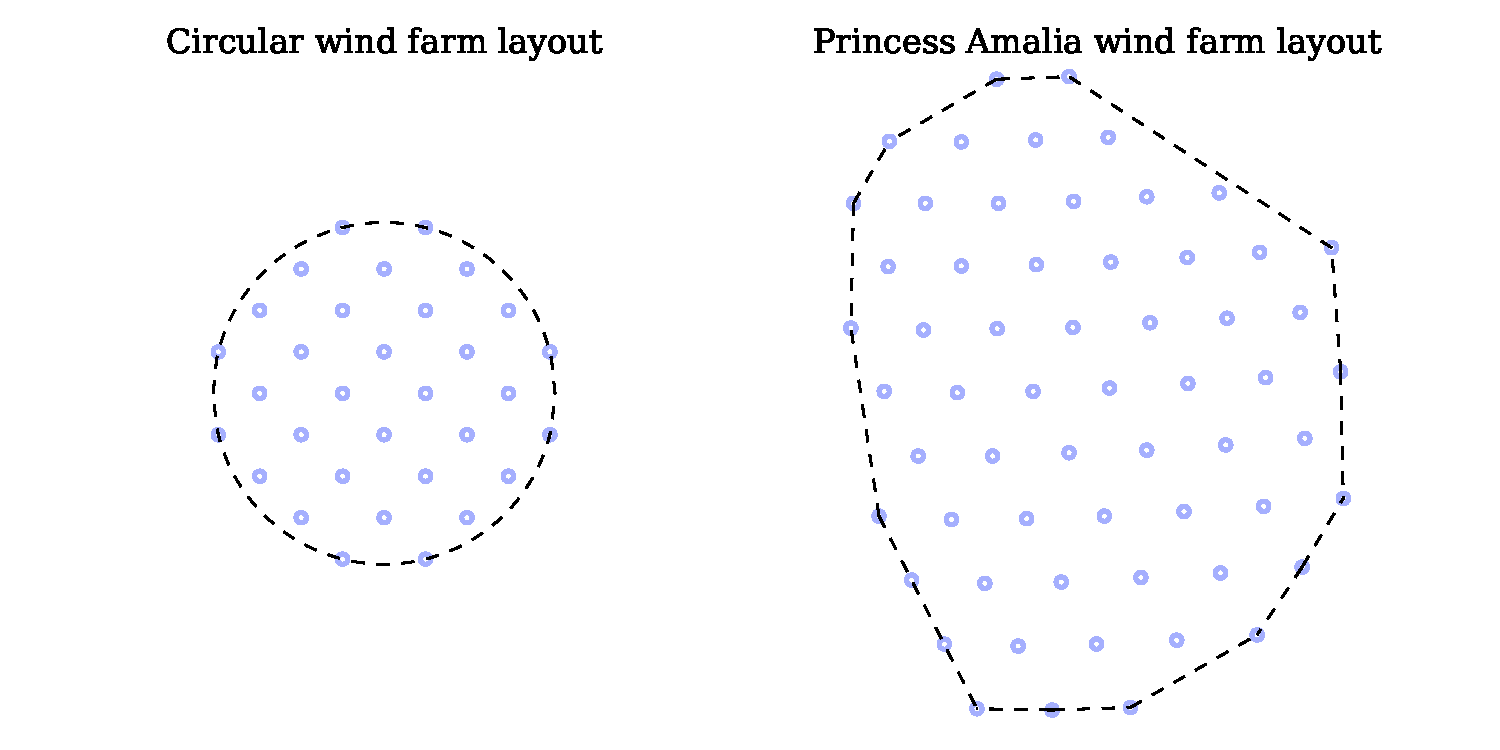
\includegraphics[width=0.7\textwidth]{Figures/baseline_layouts.pdf}
  \caption{\label{layouts} The two different wind farm designs that were optimized. On the left is a contrived circular wind farm design with 32 turbines. On the right is the Princess Amalia wind farm, an offset grid design with 60 wind turbines. }
\end{figure}
%
\begin{figure}[htbp]
  \centering
  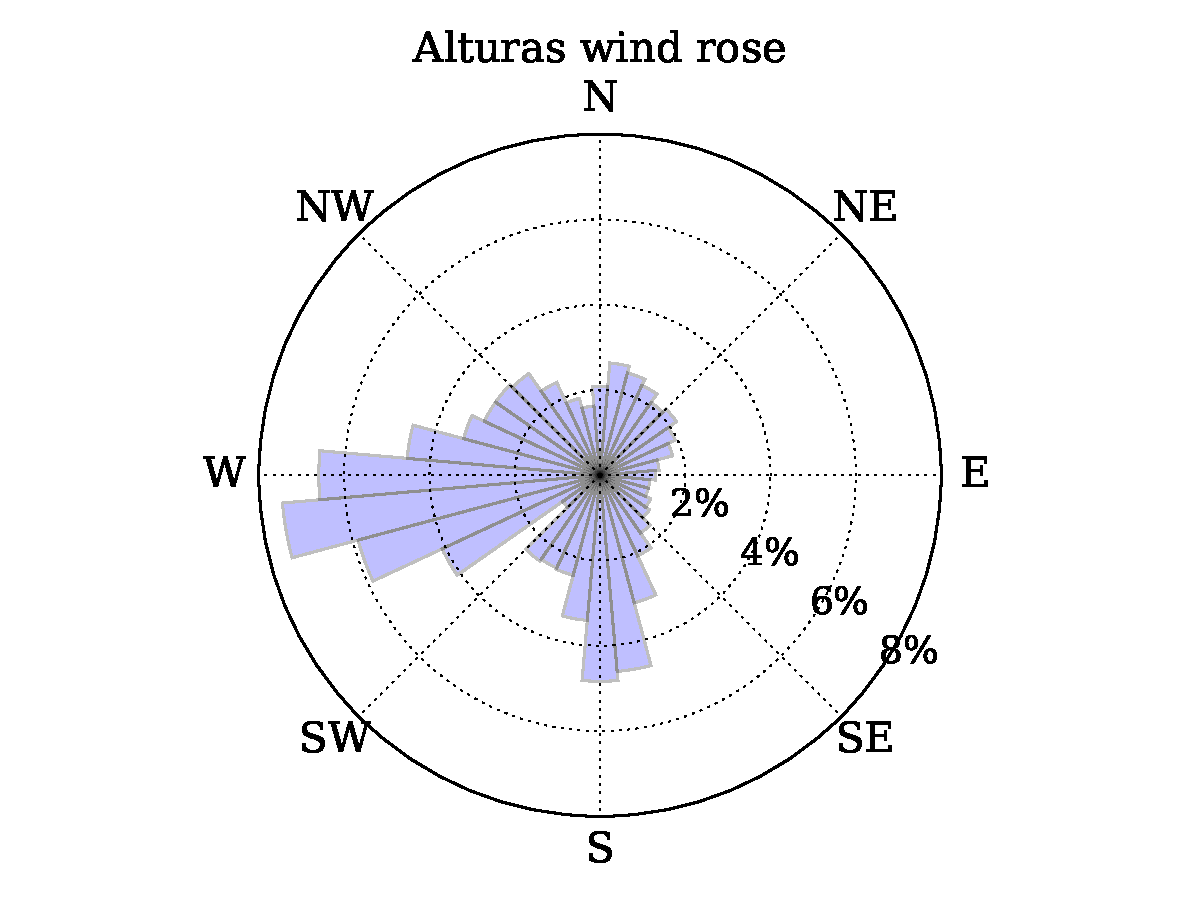
\includegraphics[width=0.49\textwidth]{Figures/alturas_rose.pdf}
  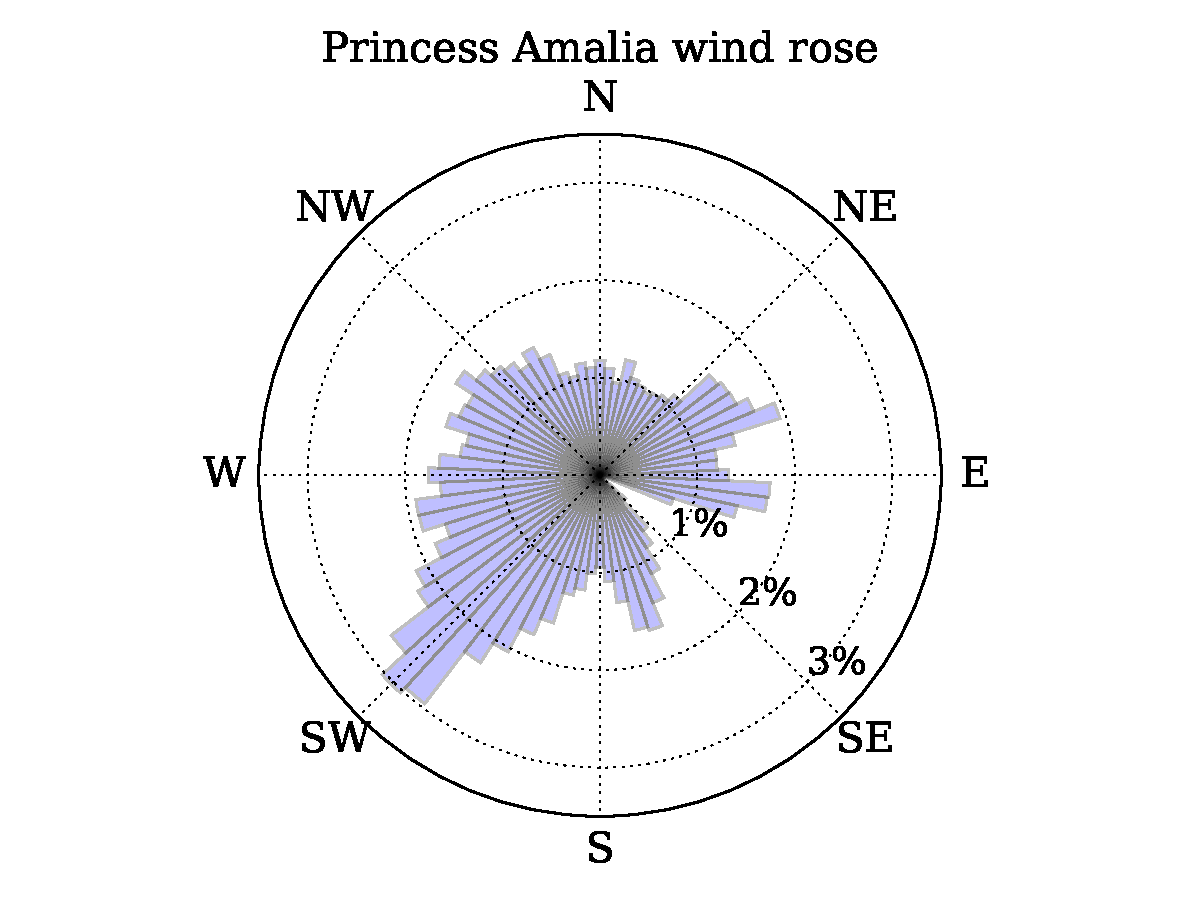
\includegraphics[width=0.49\textwidth]{Figures/amalia_rose.pdf}
  \caption{\label{wind_roses} On the left, the wind direction distribution in Alturas, California, separated into 36 bins, every 10 degrees. On the right, the wind direction distribution of the Princess Amalia Wind Farm, separated into 72 bins, every 5 degrees.}
\end{figure}
%
\begin{figure}[htbp]
  \centering
  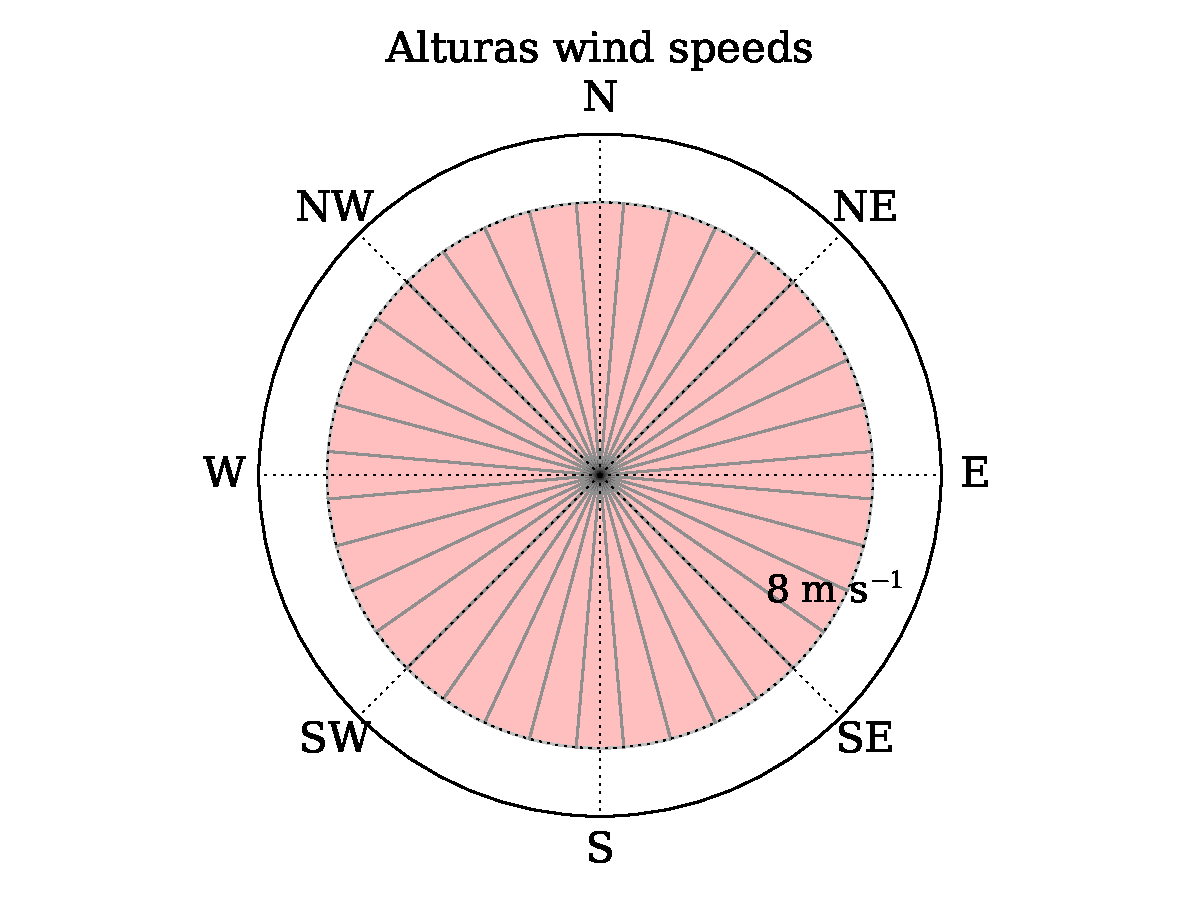
\includegraphics[width=0.49\textwidth]{Figures/alturas_speeds.pdf}
  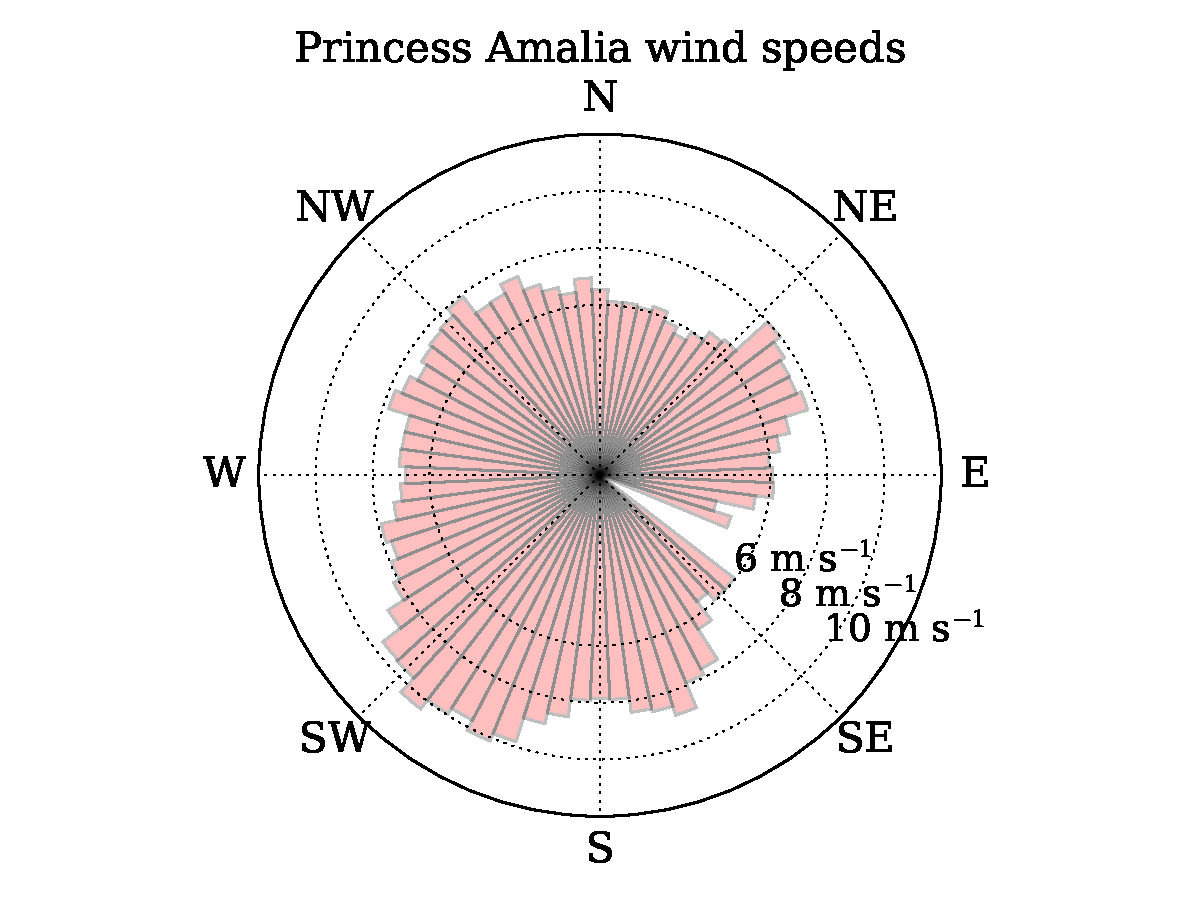
\includegraphics[width=0.49\textwidth]{Figures/amalia_speeds.pdf}
  \caption{\label{wind_speeds} On the left, the assumed directionally averaged wind speeds for Alturas, California, separated into 36 bins, every 10 degrees. Each direction is assumed to have an average wind speed of 8 meters per second. On the right, the directionally averaged wind speeds of the Princess Amalia Wind Farm, separated into 72 bins, every 5 degrees.}
\end{figure}


We optimized each of the wind farms shown in Fig. \ref{layouts} with three different wind shear exponents (0.075, 0.175, 0.275), and three different spacing multipliers (0.5, 1.0, 1.5). The wind shear exponent defines how fast the wind speed changes with height, as seen in Equation \ref{Eq:shear}. Low shear exponents are typical over open water or flat plains, while higher shear exponents exist in areas with a lot of large trees or buildings. Figure \ref{shear_profile} shows the wind speed profiles of the three shear exponents we used. For a shear exponent of 0.075, there is only an 8.6\% increase in the wind speed from the reference height of 50 meters to 150 meters. For a shear exponent of 0.175 there is a wind speed increase of 21.2\% for the same height difference, and for a shear exponent of 0.275 the wind speed increase is 35.3\% from 50 to 150 meters. We also optimized each wind farm for different turbine spacings by adjusting the turbine locations by some spacing multiplier, $\beta$.  This is simply some constant multiplied to each turbine location. The wind farm boundaries were adjusted accordingly with the spacing multipliers, meaning the radius of the circular wind farm was also multiplied by the spacing multiplier, and the convex hull of the Princess Amalia farm was applied to the adjusted turbine locations. Figure \ref{farm_spacings} shows both of the wind farms adjusted by the spacing multipliers, as well as the turbine spacing in baseline rotor diameters. As the turbine designs are optimized, these spacings (in rotor diameters) will increase or decrease according. Note that in the circular wind farm, the turbine distances are presented in the rows closely inline with the dominant wind direction (ten degrees south of west, see Fig. \ref{wind_roses}). The closest neighboring turbines are actually $\sqrt{2}/2$ multiplied by this value. 


\begin{figure}[htbp]
  \centering
  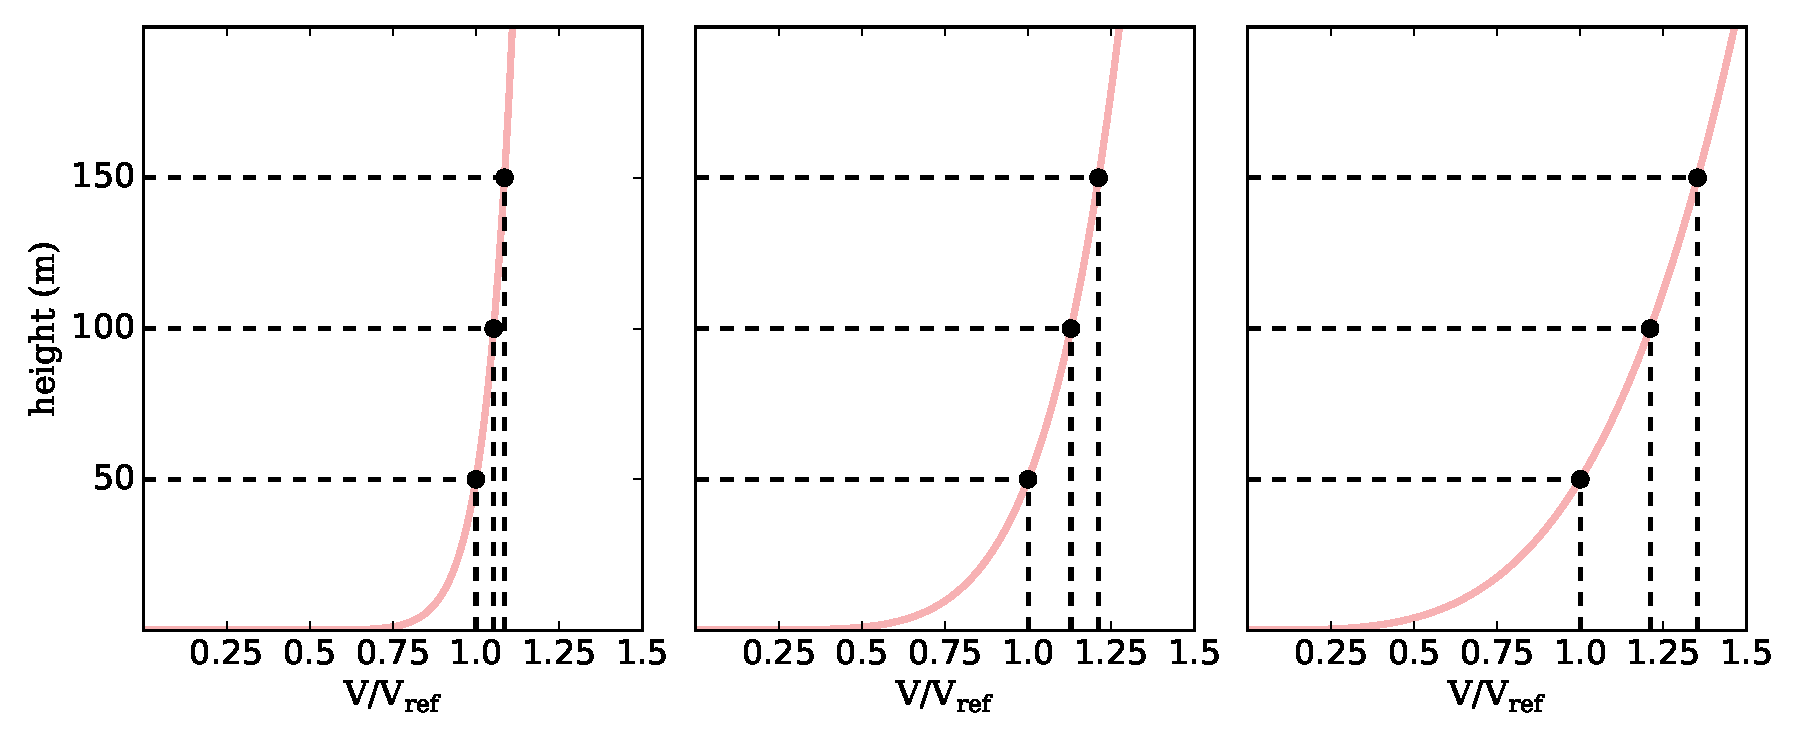
\includegraphics[width=0.7\textwidth]{Figures/shears.pdf}
  \caption{\label{shear_profile}The wind speed profiles for various wind shear exponents. With lower shear exponents the wind speed does not vary dramatically with height. For higher wind shear there is a significant wind speed increase with height.}
\end{figure}

\begin{figure}[htbp]
  \centering
  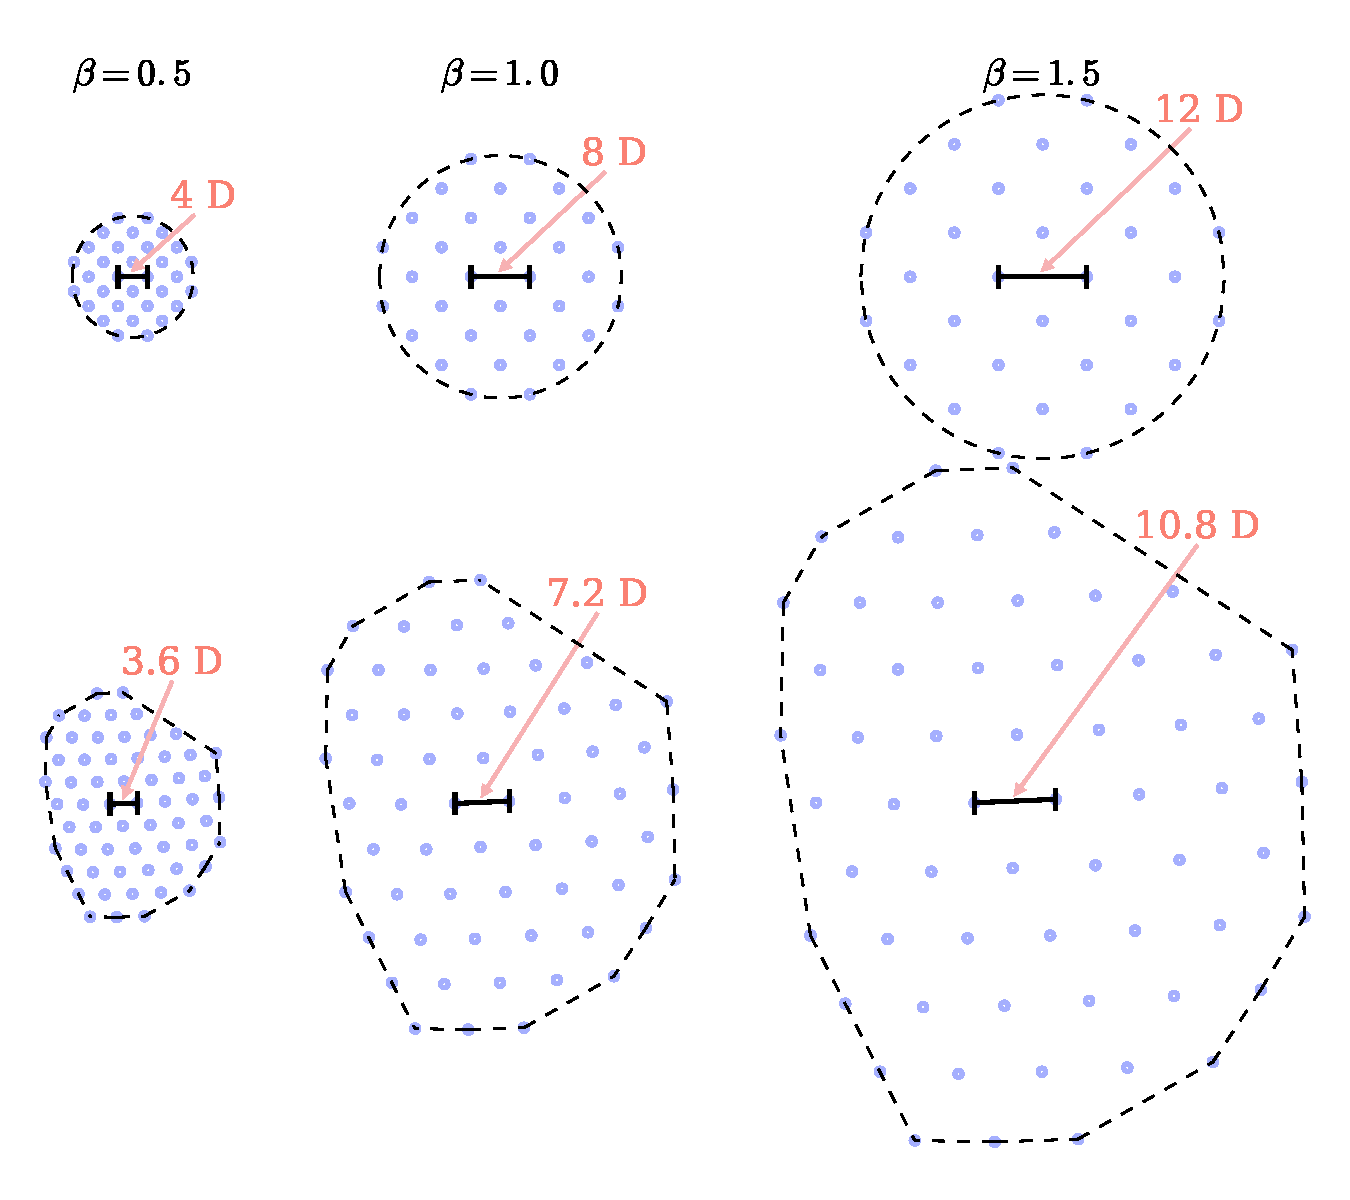
\includegraphics[width=0.7\textwidth]{Figures/spacing_multipliers.pdf}
  \caption{\label{farm_spacings}The six wind farm boundaries and associated baseline layouts optimized in this study. The same two layouts were multiplied by a spacing multiplier, $\beta=0.5,1.0,1.5$, which changed the wind farm size and the averaging spacing between wind turbines.  On the top is the 32-turbine, circular wind farm, and on the bottom is the 60-turbine, Princess Amalia wind farm. The turbine spacings, in baseline rotor diameters, are also displayed for each spacing multiplier in this figure.}
\end{figure}

The results of gradient-based optimization, especially for problems with many local minima, are sensitive to the starting location. As in most optimization problems, there is no guarantee that the solution is the global solution. The best results can be achieved with a multiple-start approach, where several different starting points are used for each condition, and the best solution is used. In our study, we ran fifty to hundreds of starting locations for each optimization case. For every optimization, we started each turbine location from the Princess Amalia or circular wind farm baseline locations in Fig. \ref{farm_spacings}, each perturbed by a random amount. All of the other design variables were initialized randomly.




\section{Results}
%\newcommand\myeq{\mkern1.5mu{=}\mkern1.5mu}


In this section we will discuss the optimization results of both wind farms, the apparent benefit of coupled turbine layout and design optimization, as well as the benefit of heterogeneous turbine design in a wind farm.
We will first present the results from the 32-turbine circular wind farm optimizations, followed by the 60-turbine Princess Amalia wind farm optimizations. For each wind farm, we present the optimal COE results for each wind shear exponent and spacing multiplier combination (Figs. \ref{circular_results} and \ref{amalia_results}). Each combination has four points, representing a layout optimization performed with the baseline turbine design, a turbine design optimized in isolation followed by layout optimization, coupled layout and homogeneous turbine design optimization, and finally coupled layout and turbine design optimization with two different turbine groups. 
We next show the optimal rotor diameters and hub heights of the turbines optimized in isolation (Figs. \ref{circular_turbines_seq} and \ref{amalia_turbines_seq}), the rotor diameters and hub heights of the coupled design-and-layout optimization, with homogeneous turbine design (Figs. \ref{circular_turbines_1} and \ref{amalia_turbines_1}), the rotor diameters and hub heights of the coupled design-and-layout optimization, with two different turbine groups (Figs. \ref{circular_turbines} and \ref{amalia_turbines}), and the optimal rated powers of the coupled design-and-layout optimization, for the optimizations with both one and two turbine groups (Figs. \ref{circular_power} and \ref{amalia_power}).
% Figures \ref{circular_turbines} and \ref{amalia_turbines} show the turbine heights and rotor diameters in the optimization cases with two different turbine groups. Figures \ref{circular_power} and \ref{amalia_power} show the optimal power rating of each turbine group in the optimization cases with two different height groups. 



\subsection{Circular Wind Farm Optimization}

Figure \ref{circular_results} shows the optimal COE results for the circular wind farm. As shown in the legend, the white points represent the layout-only optimization, the gray indicate the sequential-turbine-design-then-layout optimization, the black points show the coupled-turbine-design-and-layout optimization, and the half blue and pink points represent the couple design and layout optimization with two turbine groups.  As expected, the general trends for all optimizations run show that the higher wind speed from high wind shear results in a lower, superior optimal COE. Additionally, the widely spaced wind turbines indicated by the larger spacing multipliers also result in lower COE due to less wake interaction between turbines. 

\begin{figure}[htbp]
  \centering
  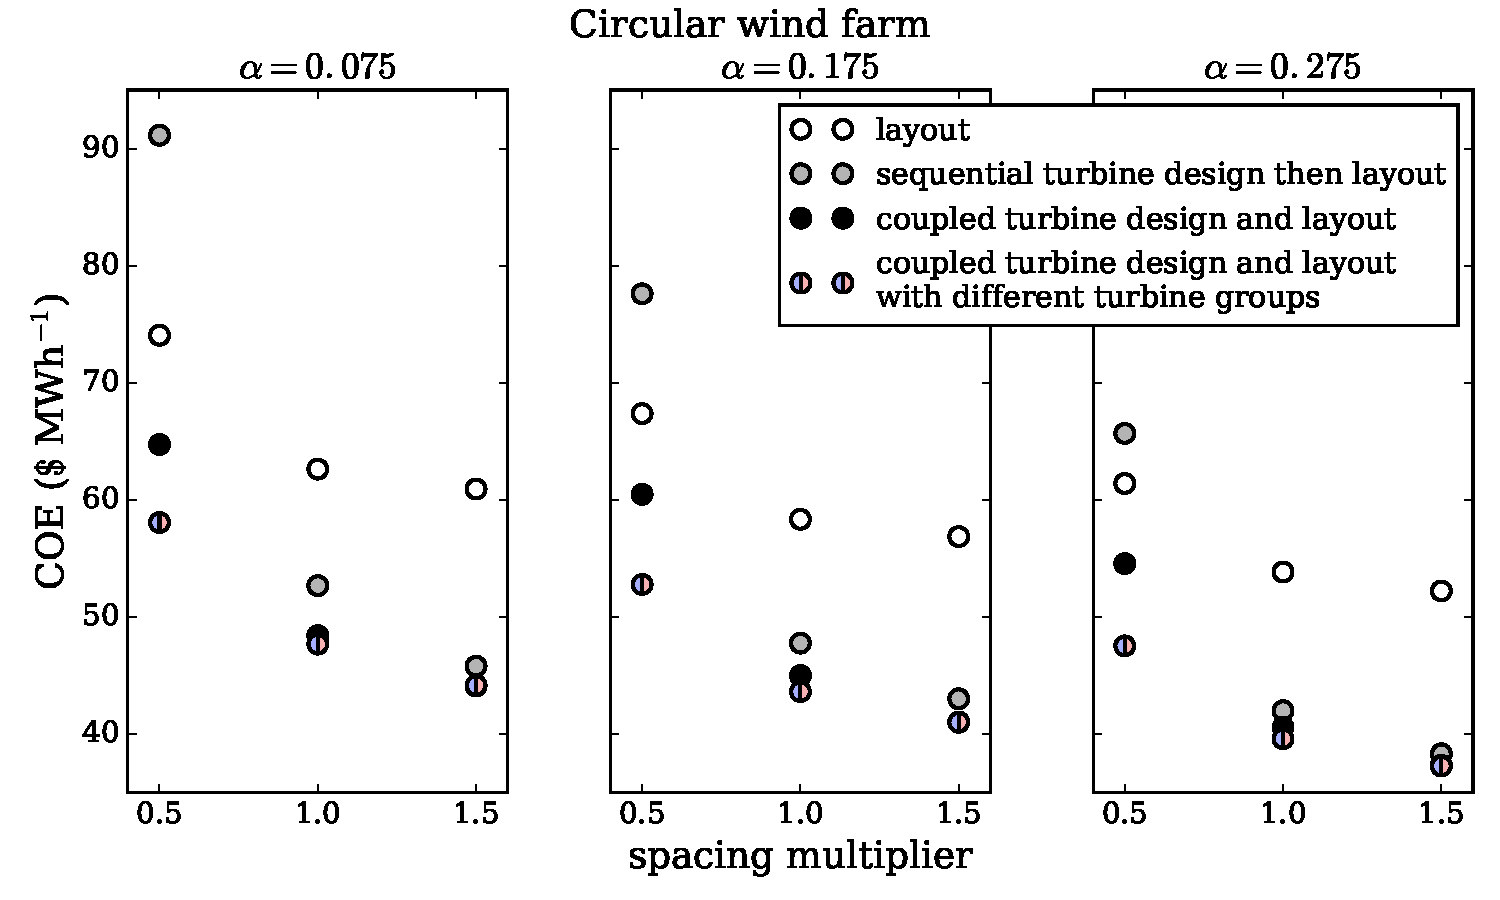
\includegraphics[width=0.8\textwidth]{Figures/circular_results1.pdf}
  \caption{\label{circular_results} The optimal COE results for the circular wind farm layout with 32 turbines. Each of the subfigures corresponds to optimization runs with a different shear exponent, from left to right $\alpha=0.075,0.175,0.275$. Within each subfigure, the x axis shows the size of the wind farm based on the spacing multiplier, from left to right $\beta=0.5,1.0,1.5$. The different points represent the layout optimization, sequential turbine-design-then-layout optimization, coupled layout-and-turbine-design optimization with homogeneous turbine design throughout the farm, and layout-and-turbine-design optimization with two different turbine design groups.}
\end{figure}

\subsubsection{Sequential Turbine Design then Layout Optimization}
The gray dots show the optimal COE results for a sequential optimization. First, a turbine was designed for minimal COE in isolation with the freestream wind conditions. This turbine design was then used in the wind farm where the layout was optimized. 
The rotor diameter was constrained such that the turbine spacing constraints would be satisfied in the baseline farm where the turbine would be installed. This was only applicable for the smallest wind farms, where $\beta=0.5$. 
For each shear exponent, the optimal turbine design was the maximum rotor diameter and turbine rating allowed by the optimizer.
%: 160 meters and 10 megawatts. 
%The optimal height increased with the shear exponent: 90 meters, 147 meters, and 155 meters for the shear exponents of 0.075, 0.175, and 0.275, respectively.
Figure \ref{circular_turbines_seq} shows the optimal isolated turbine designs for each shear exponent and spacing multiplier, as well as the baseline turbine design. Because these turbines are optimized in isolation, the designs for $\beta=1.0,1.5$ are the same. The only affect the spacing multiplier has on the design is a possible maximum rotor diameter (as in the case of $\beta=0.5$).
When these optimized turbine designs are used in each wind farm instead of the baseline turbine design, there is a large COE improvement for the spacing multipliers of $\beta=1.0, 1.5$. For $\beta=1.0$, COE decreases 15.9--22.0\% compared to an optimized wind farm with the baseline turbine design. For $\beta=1.5$ the COE decrease is even larger, 24.8--26.6\% across all shear exponents. 
%For the smallest wind farm, $\beta=0.5$, the turbine design optimized in isolation results in an infeasible farm layout. The rotor diameter is so large and the farm area so small that no layout is possible where the turbine spacing constraints are satisfied. However, even when the turbine spacing constraints were removed, this sequential turbine-design-then-layout optimization resulted in a worse COE for shear exponents of $\alpha=0.075,0.175$ compared to the layout-only optimization, and only a slightly better COE (2.3\%) for $\alpha=0.275$. 
For the smallest wind farm, $\beta=0.5$, the turbine design optimized in isolation results in an extremely inefficient wind farm. When in the wind farm environment, exposed to much lower average wind speeds, this design results in a COE that is much worse than the baseline turbine design. The expense from a bigger and taller turbine, coupled with the strong wake interactions among turbines that are so closely spaced means that for this wind farm, optimizing the turbine in isolation actually decreases the wind farm performance. 

\begin{figure}[htbp]
  \centering
  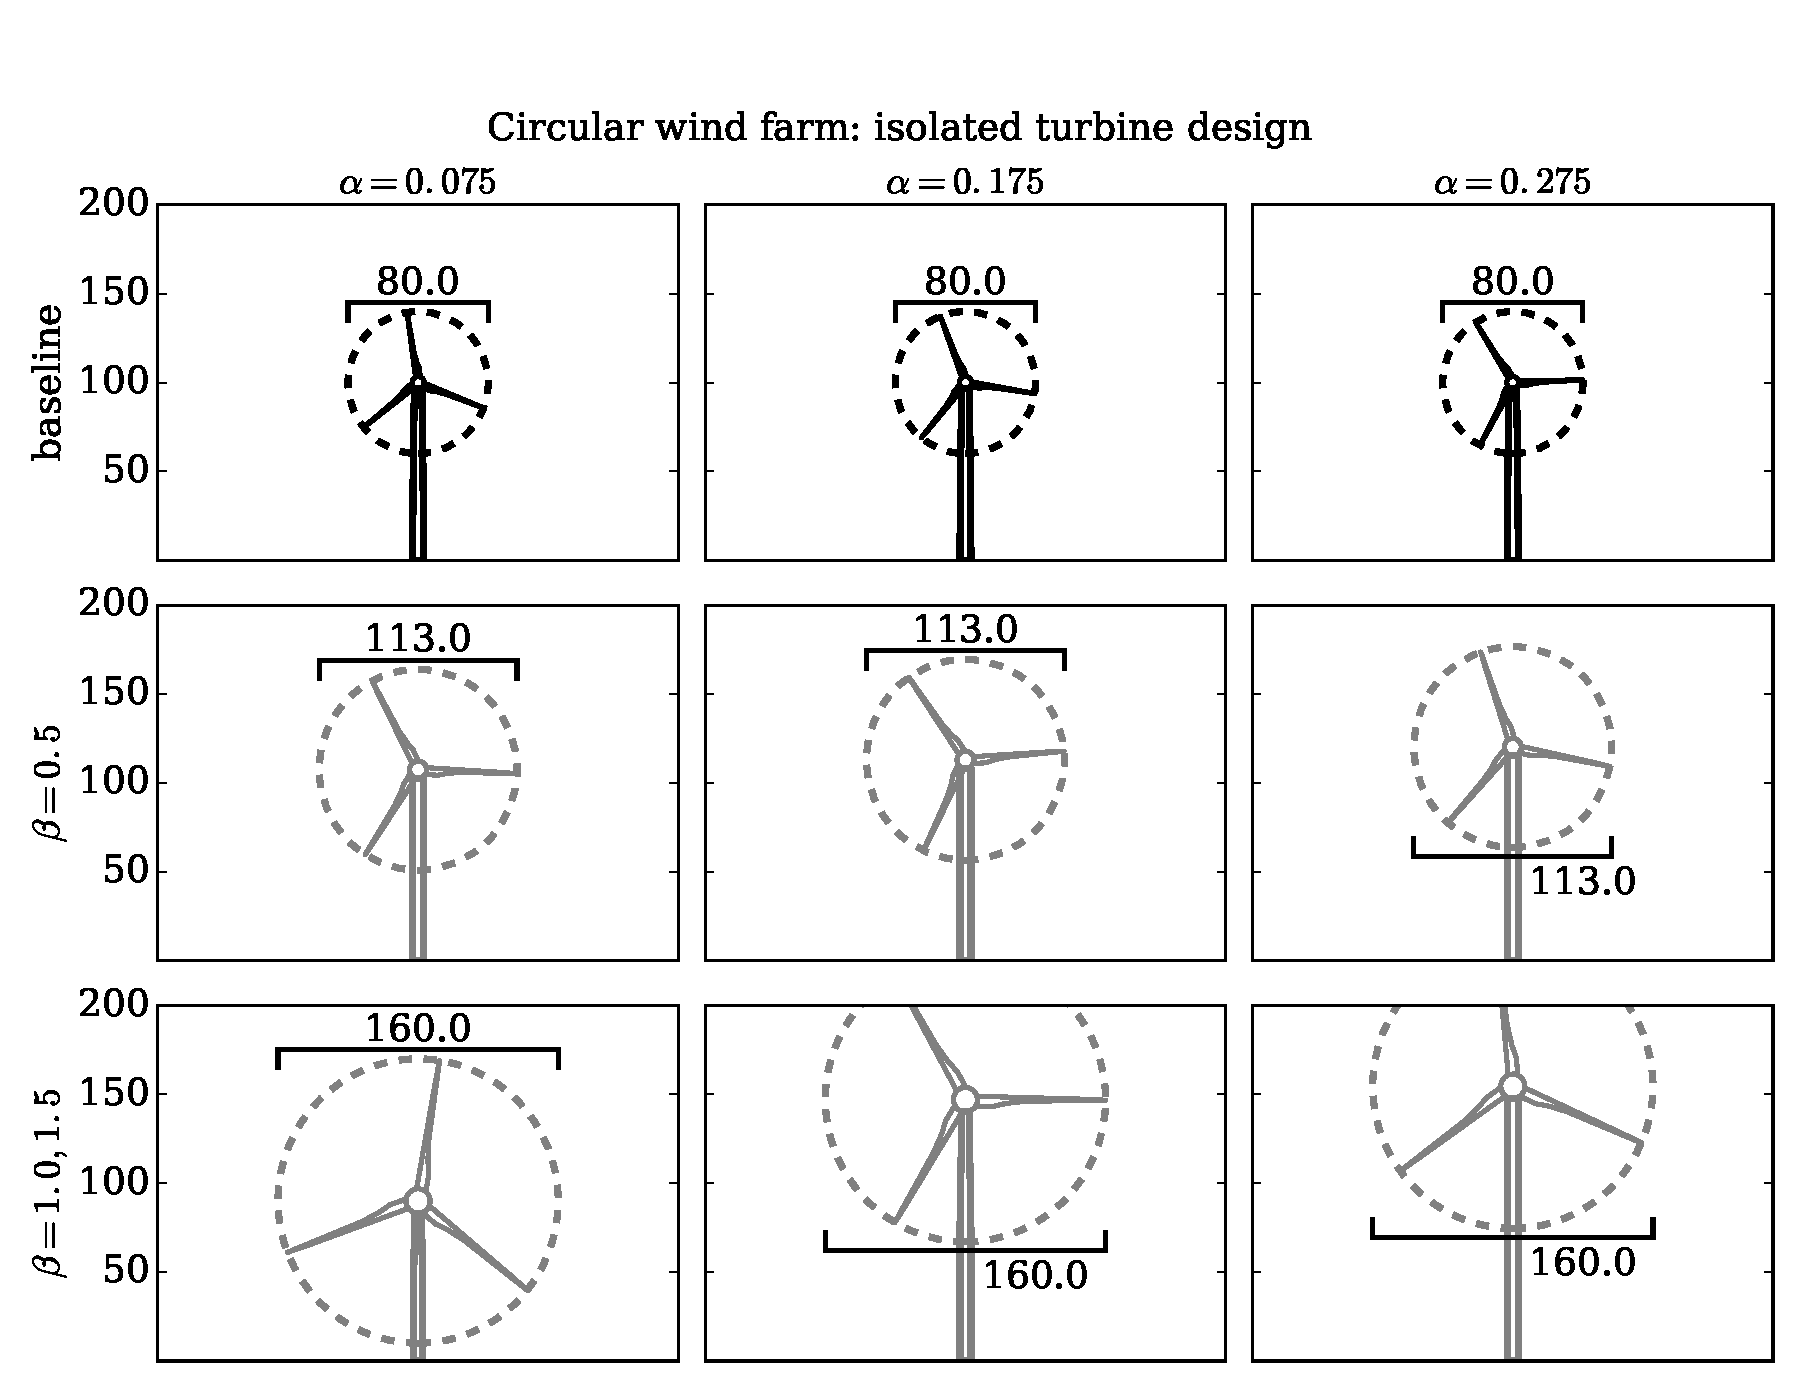
\includegraphics[width=0.8\textwidth]{Figures/turbineSizesCircular_sequential.pdf}
  \caption{\label{circular_turbines_seq} The optimal turbine heights and rotor diameters for the isolated turbine design optimization for the circular farm wind conditions. These designs were then used in the sequential turbine-design-then-layout optimizations. The columns, from left to right, show the turbines optimized for $\alpha=0.075,0.175$, and $0.275$. The rows, from top to bottom, show the baseline turbine design, the turbine optimized for the small wind farm ($\beta=0.5$), and the turbine designs for the larger wind farms ($\beta=1.0,1.5$)}
\end{figure}


\subsubsection{Coupled Turbine Design and Layout Optimization}
Next we will discuss the optimization results of the coupled turbine-design-and-layout optimizations, represented by the black dots in Fig. \ref{circular_results}. For every shear exponent and spacing multiplier, there is a large benefit to performing the coupled turbine-design-and-layout optimization compared to the layout-only optimization. Additionally, and more importantly, the coupled optimization results in appreciably lower COE than the sequential design-then-layout optimization. Obviously for a spacing multiplier of $\beta=0.5$, the coupled optimization is far superior to the sequential in that it results in a feasible wind farm. For the spacing multiplier of $\beta=1.0$, 
% which results in feasible wind farms for the sequential optimizations as well as the coupled optimizations, 
compared to the sequential optimizations, coupled optimization results in an additional 6.82\%, 4.75\%, and 2.65\% COE improvement from layout only optimization for shear exponents $\alpha=0.075, 0.175,$ and $0.275$, respectively. For the largest wind farm, $\beta=1.5$, the coupled optimization results in an additional 2.78\%, 3.50\%, and 1.88\% COE improvement compared to the sequential case. 

There are several conclusions we can make from both the sequential and coupled turbine design and layout optimizations. First, and most apparent, optimizing turbine design results in a much better wind farm than a farm in which the turbines are selected arbitrarily or a priori. Second, and more importantly, optimizing turbine design coupled with the turbine layout is significantly better than optimizing the turbine design for the freestream wind conditions alone. In a wind farm, turbines rarely experience the freestream wind conditions as they are often waked by the other turbines in the farm. Therefore, the optimal turbine design is based on on average slower wind speeds than the freestream wind. This results in turbines with smaller hub heights, rotor diameters, and rated powers. 

Figure \ref{circular_turbines_1} shows the optimal rotor diameters and hub heights for the coupled turbine design and layout optimizations. For a spacing multiplier $\beta=0.5$, the turbines are very close together and in general are heavily waked. Thus to satisfy spacing constraints and because the average wind speed is very low, the optimal rotor diameter is small: about 90 meters. When the turbines are spaced farther apart, shown for the larger spacing multipliers, the optimal rotor diameter is much larger: closer to 120--130 meters. In these farms, wake interactions are not as severe, meaning that the extra power production from larger rotors is worth the extra turbine capital cost. Also notice the trend of the optimal turbine height with wind shear exponent. For a low wind shear exponent, $\alpha=0.075$, the wind speed does not drastically change with height (see Fig. \ref{wp075}). Therefore, for this wind condition it is desireable to have short hub heights with a lower turbine capital cost. For the higher shear exponents, $\alpha=0.175,0.275$, the wind speed increases much more with height (See Figs. \ref{wp175} and \ref{wp275}). In these cases, for every spacing multiplier, the extra cost of building the taller turbines is made up for in the additional power produced from the high wind speeds. Note that a larger rotor diameter reduces the relative spacing between turbines in the farm, as the original spacing was based on a diameter of 80 meters.


\begin{figure}[htbp]
  \centering
  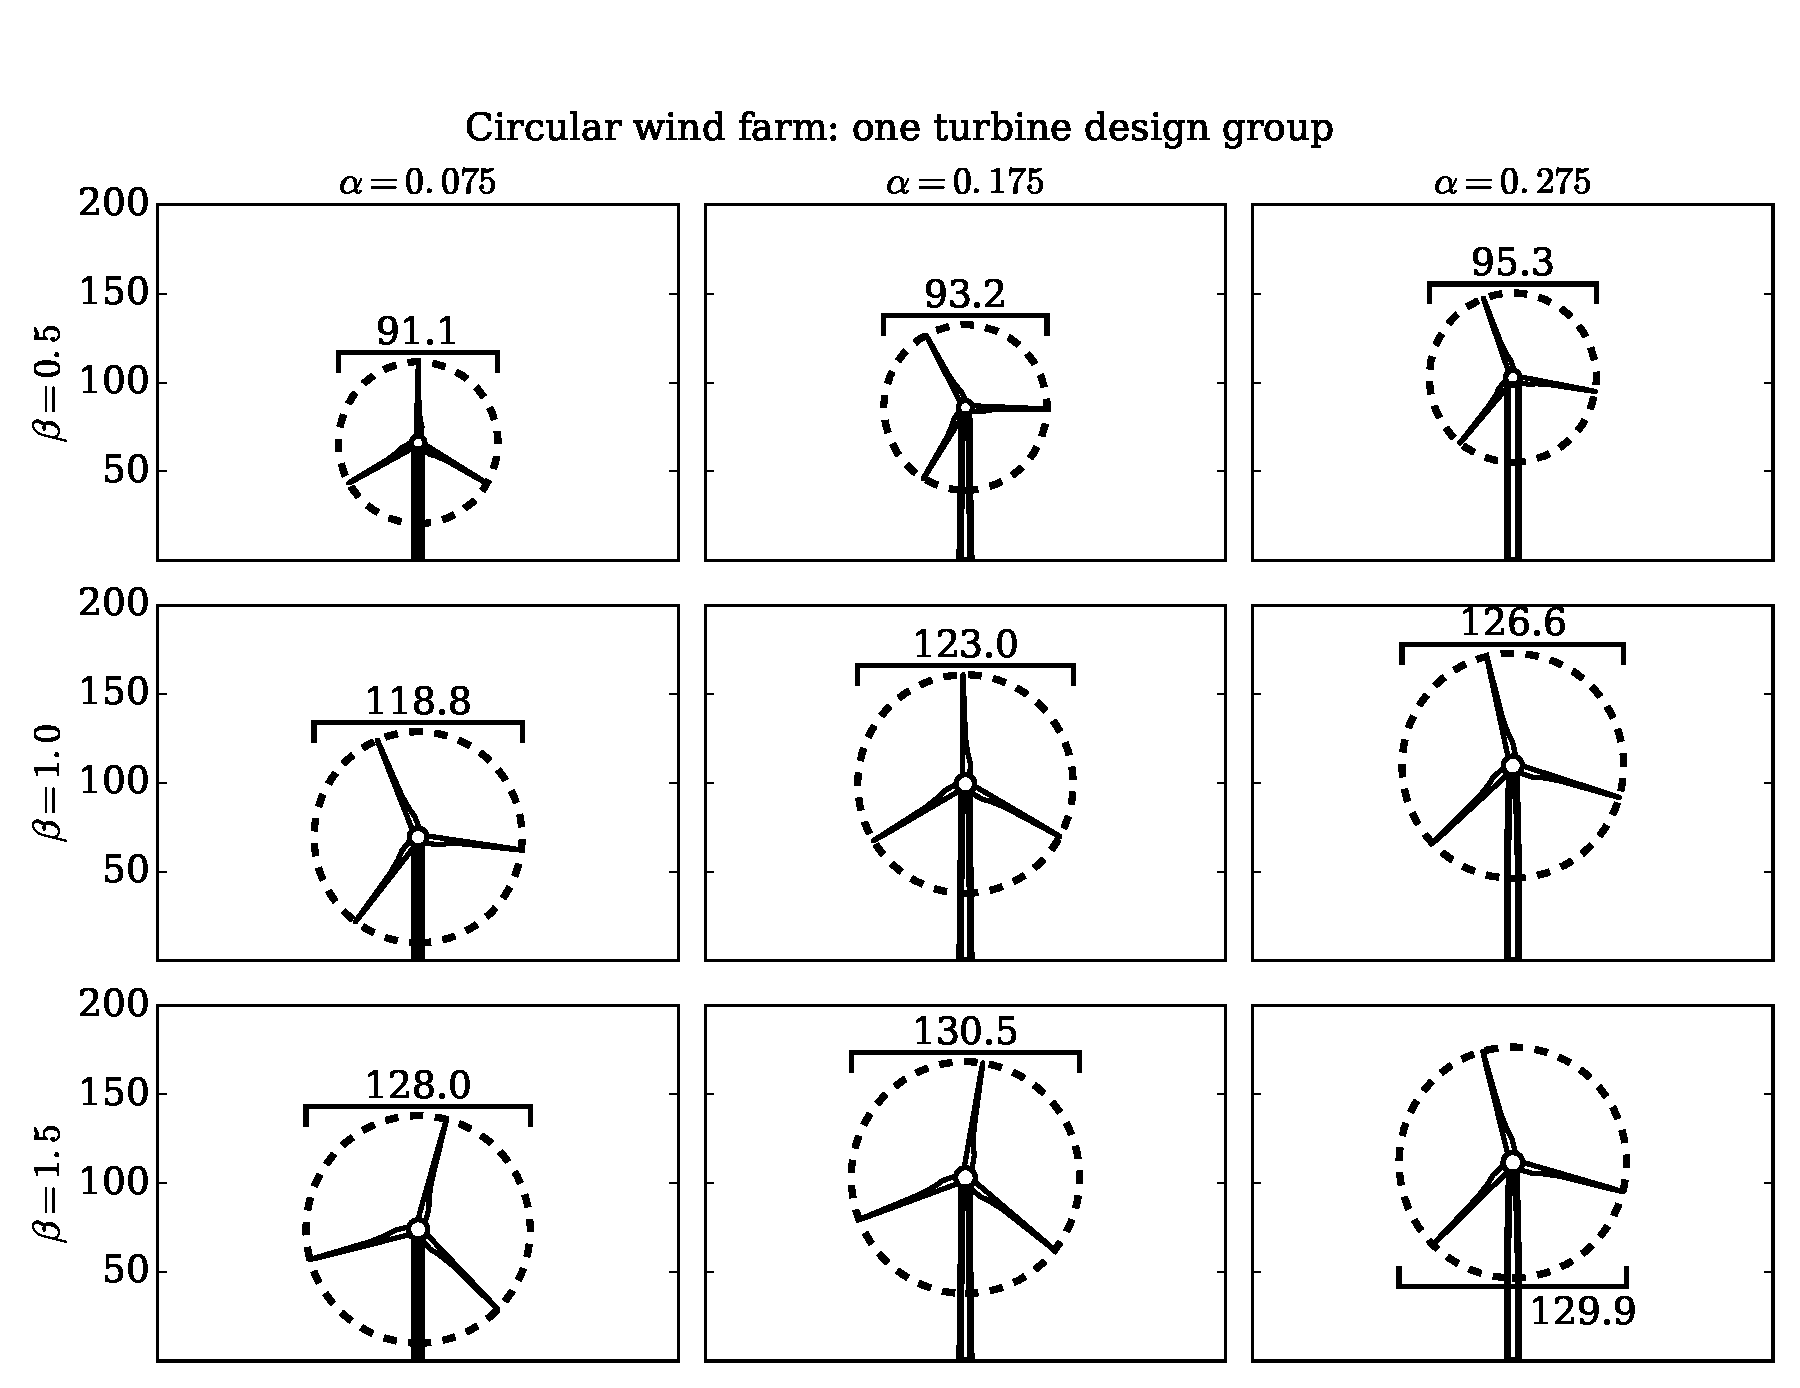
\includegraphics[trim={0.5cm 0.3cm 0.3cm 1.75cm},clip,width=0.8\textwidth]{Figures/turbineSizesCircular_1.pdf}
  \caption{\label{circular_turbines_1} The optimal turbine heights and rotor diameters for the optimization runs with coupled layout and turbine design with homogeneous turbine design throughout the circular wind farm. Each column shows a different shear exponent, with $\alpha=0.075,0.175,0.275$ from left to right. Each row shows a different farm spacing multiplier, with $\beta=0.5,1.0,1.5$ from top to bottom.}
\end{figure}

In Fig. \ref{circular_power}, the black points show the optimal rated powers for the turbines in each optimization case. Notice that the optimal rated power scales with the turbine rotor diameter and hub height. Higher turbine rating is expensive. Therefore, the small rotors and short turbines, which are more heavily waked and don't produce as much power, do not require a large power rating. The extra cost is not justified by a very slight increase in power. For the high shear exponents and spacing multipliers, the turbines are exposed to faster wind speeds. These turbines are bigger and taller, and the extra power production from raising the rated pwoer is worth the additional cost.



\subsubsection{Coupled Turbine Design and Layout Optimization with Two Turbine Groups}

Now we will discuss the most interesting case, the coupled turbine design and layout optimization with two different turbine groups. The optimal COE results of these optimziations are shown with the blue and pink points in Fig. \ref{circular_results}. Most visibly, for the smallest spacing multiplier, $\beta=0.5$, there is a large COE improvement for the hetergenous turbine design optimizations compared to the farms with homogeneous turbine design (shown by the black points in Fig. \ref{circular_results}). For this spacing multiplier, the heterogenous turbine design farms reduce COE by 21.6\%, 21.67\%, and 22.6\% compared to the layout-only optimization for shear exponents of $\alpha=0.075,0.175$, and $0.275$, respectively. The coupled optimizations with one turbine group reduce COE by 12.59\%, 10.24\%, and 11.15\%. For the smallest spacing multiplier, optimizing turbine design and layout with two turbine groups reduces COE by an additional 9--11.45\% compared to just one turbine group. For the spacing multiplier $\beta=1.0$, the coupled optimization with two turbine groups results in an additional 1.16--2.35\% COE decrease compared to with one turbine group. This is much smaller than the more tightly packed wind farms, but still non-negligible. For the spacing multiplier $\beta=1.5$, the optimization with two turbine groups results in only an additional 0--0.12\% COE decrease, indicating that when the turbines are spread very far apart there is no benefit to allowing multiple turbine designs in the same farm.

The two different rotor designs in the same wind farm help to improve COE by reducing the wake interaction between wind turbines. By combining tall and short turbines, with large and small rotor sizes, there are more dimensions that the optimizer can manipulate to avoid wakes and improve performance. For the tightly packed wind farms, the turbine layout is greatly limited by the turbine spacing constraints. Additionally, as the turbines are closer together, the wakes greatly reduce the wind speed as they have not had an opprtunity to mix with the freesteam air. Both of these factors mean there is a large benefit to avoiding the wakes of other turbines by any means possible. For the larger wind farms where the turbines are spaced farther apart, the wakes are not as detrimental and there is more area in which to avoid wakes in the horizontal plane without needing to change hub height or rotor diameter. In these cases, the heterogenous turbine designs are not as beneficial.

Figure \ref{circular_turbines} shows the optimal rotor diameter and hub height of each turbine group for these cases of coupled turbine design and layout optimization with two different groups. For the spacing multiplier $\beta=0.5$, when the turbines are very close together, there is a large difference in both the rotor diameter and hub height of each turbine group. Group 1 is extremely small and short, smaller than even the baseline rotor diameter, while Group 2 is much larger. Even if turbines from each group were right next to each other, there would be minimal wake interaction between the turbines. For the small wind farms, the sacrifice in power that comes from one very small and short turbine is made up for in the decreased wake inteference between turbine groups. Essentially, having two different turbine groups doubles the effective spacing between turbines, because turbines in different groups do not affect each other. For a larger spacing multiplier of $\beta=1.0$, each turbine group is still remarkably different in size and height. The turbines are larger than they were for the smallest wind farm because the average wind speed is faster when the turbines are spread farther apart. Notice that, compared to the optimized turbines for $\beta=0.5$, the smaller turbines when $\beta=1.0$ are larger and overlap more with the taller, bigger turbines. In this case, the power increase from bigger rotor diameters outweighs the benefit gained from reducing wake interference. 

The turbine sizes for the largest wind farm, $\beta=1.5$, demonstrate the multi-modality of the wind farm optimization problem. For this spacing multiplier, each turbine group is much more similar than in the previous wind farm sizes. For the lowest shear exponent, $\alpha=0.075$, both turbine groups are almost identical. For $\alpha=0.175,0.275$, there is some difference in each rotor diameter and hub height, although the difference is not as pronounced as it was for the smaller wind farms. However, Fig. \ref{circular_results} shows that for $\beta=1.5$ the optimal COE from coupled turbine design and layout optimization is the same with one and two height groups. So, a wind farm with the homogeneous turbine design shown in the bottom row of Fig. \ref{circular_turbines_1}, and a wind farm with two different turbine designs shown in the bottom row of Fig. \ref{circular_turbines} result in the same COE. The same optimal result is achieved with drastically different farms, each with different turbines and layouts.  

\begin{figure}[htbp]
  \centering
  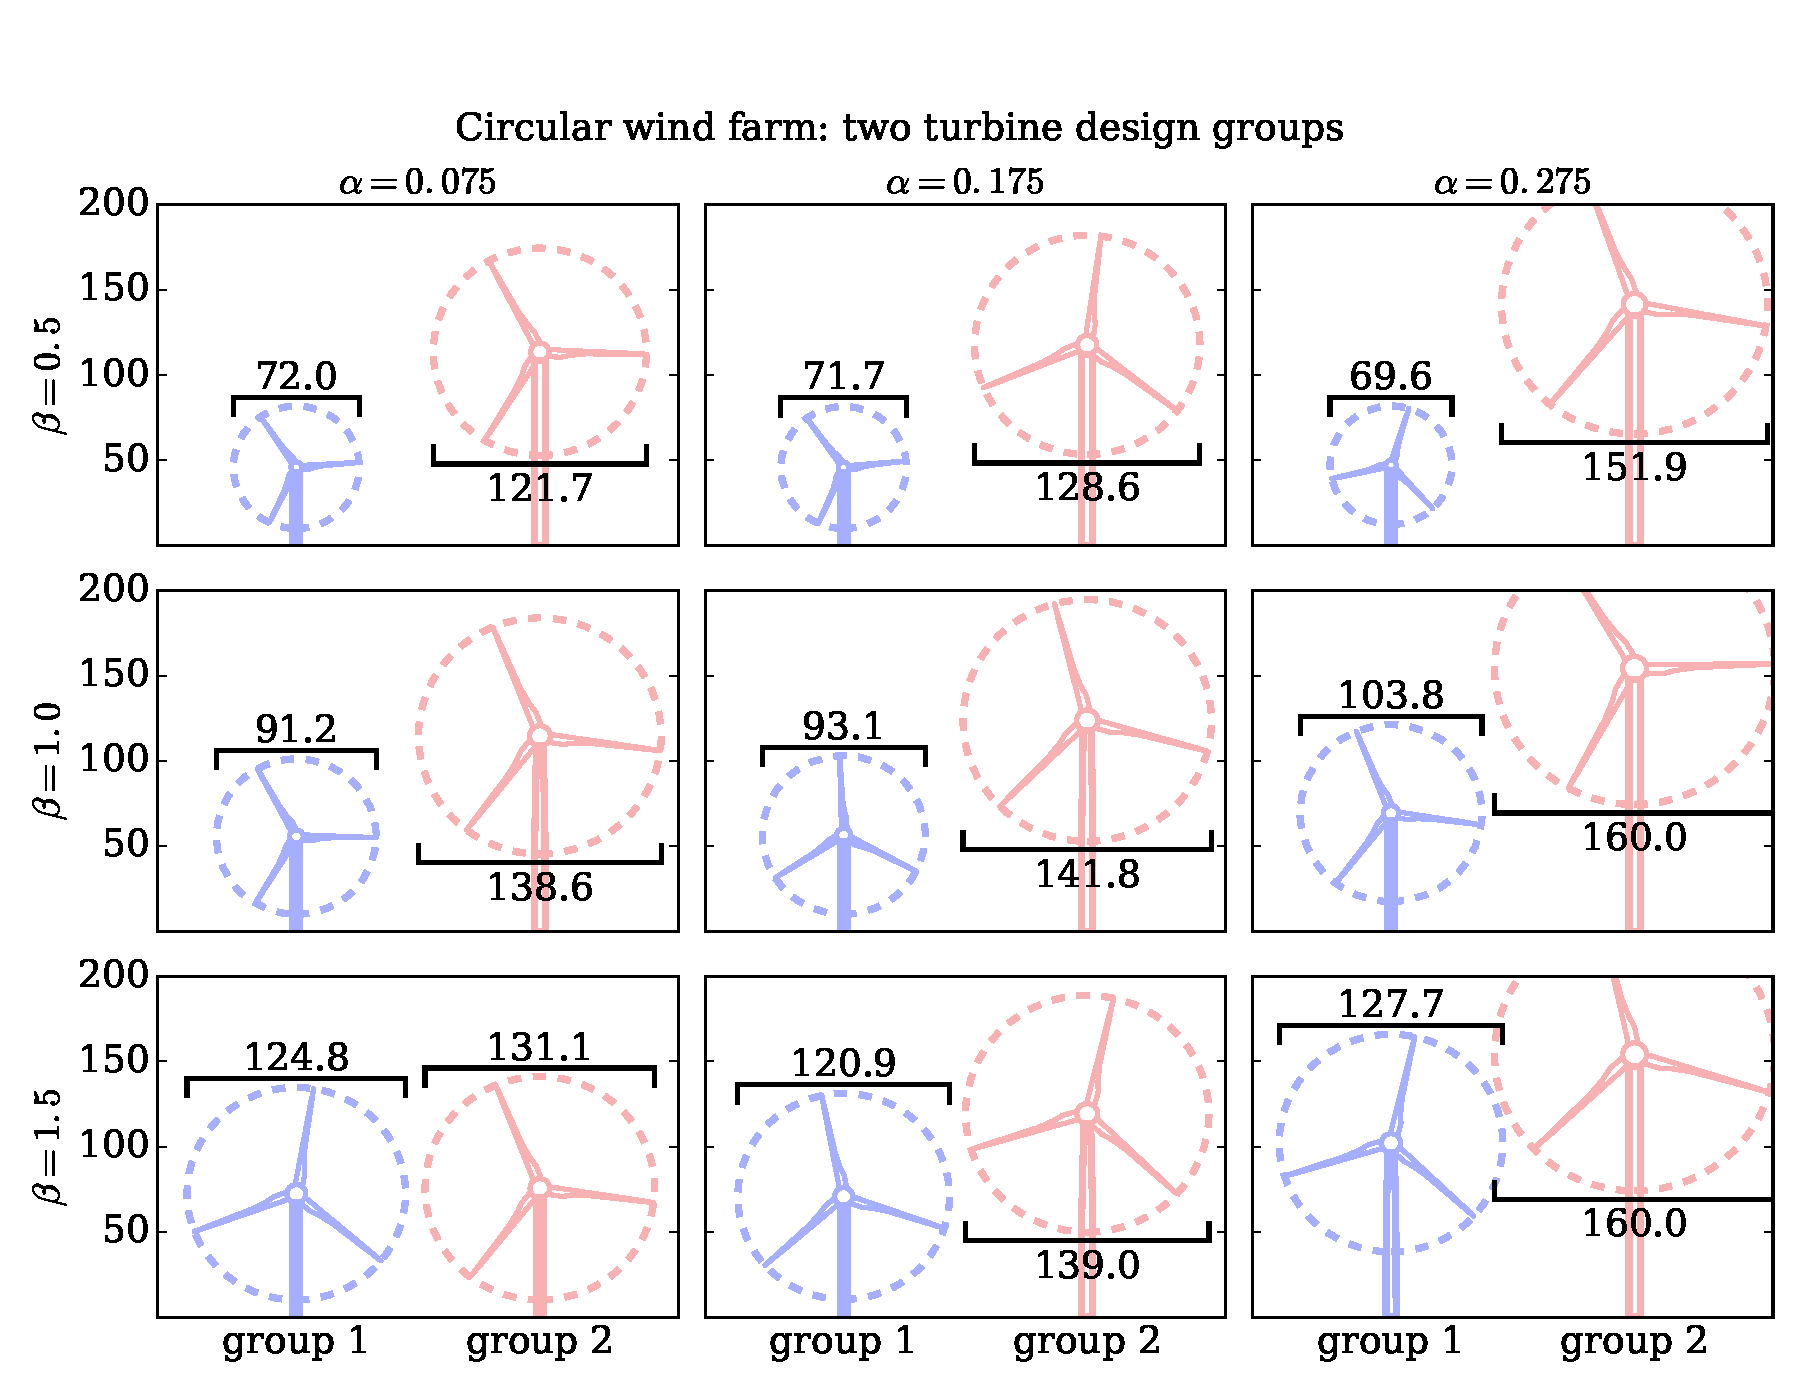
\includegraphics[trim={0.5cm 0.3cm 0.3cm 1.75cm},clip,width=0.8\textwidth]{Figures/turbineSizesCircular_2.pdf}
  \caption{\label{circular_turbines} The optimal turbine heights and rotor diameters for the optimization runs with coupled layout and turbine design with two different turbine design groups for the circular wind farm. Each column shows a different shear exponent, with $\alpha=0.075,0.175,0.275$ from left to right. Each row shows a different farm spacing multiplier, with $\beta=0.5,1.0,1.5$ from top to bottom.}
\end{figure}


Figure \ref{circular_power} shows the optimal rated power of each height group for the optimization cases with two different turbine groups. The blue and pink dots in this plot correspond to the turbines of the same color in Fig. \ref{circular_turbines}. As with the homogeneous turbine wind farm, the optimal rated power scales with the optimal turbine height and diameter. These larger, taller turbines are optimal in wind farms where they will be exposed to high wind speeds and produce large amounts of power. From a power production standpoint, it is undesirable to ever have a turbine's power limited by the rating. However, turbines with high ratings are more expensive, and not worth the cost if the turbine is generally producing low amounts of power. Therefore, the short, small turbines are optimal with a low, cheap power rating. The larger, taller turbines which produce much more electricity utilize the higher ratings. 


\begin{figure}[htbp]
  \centering
  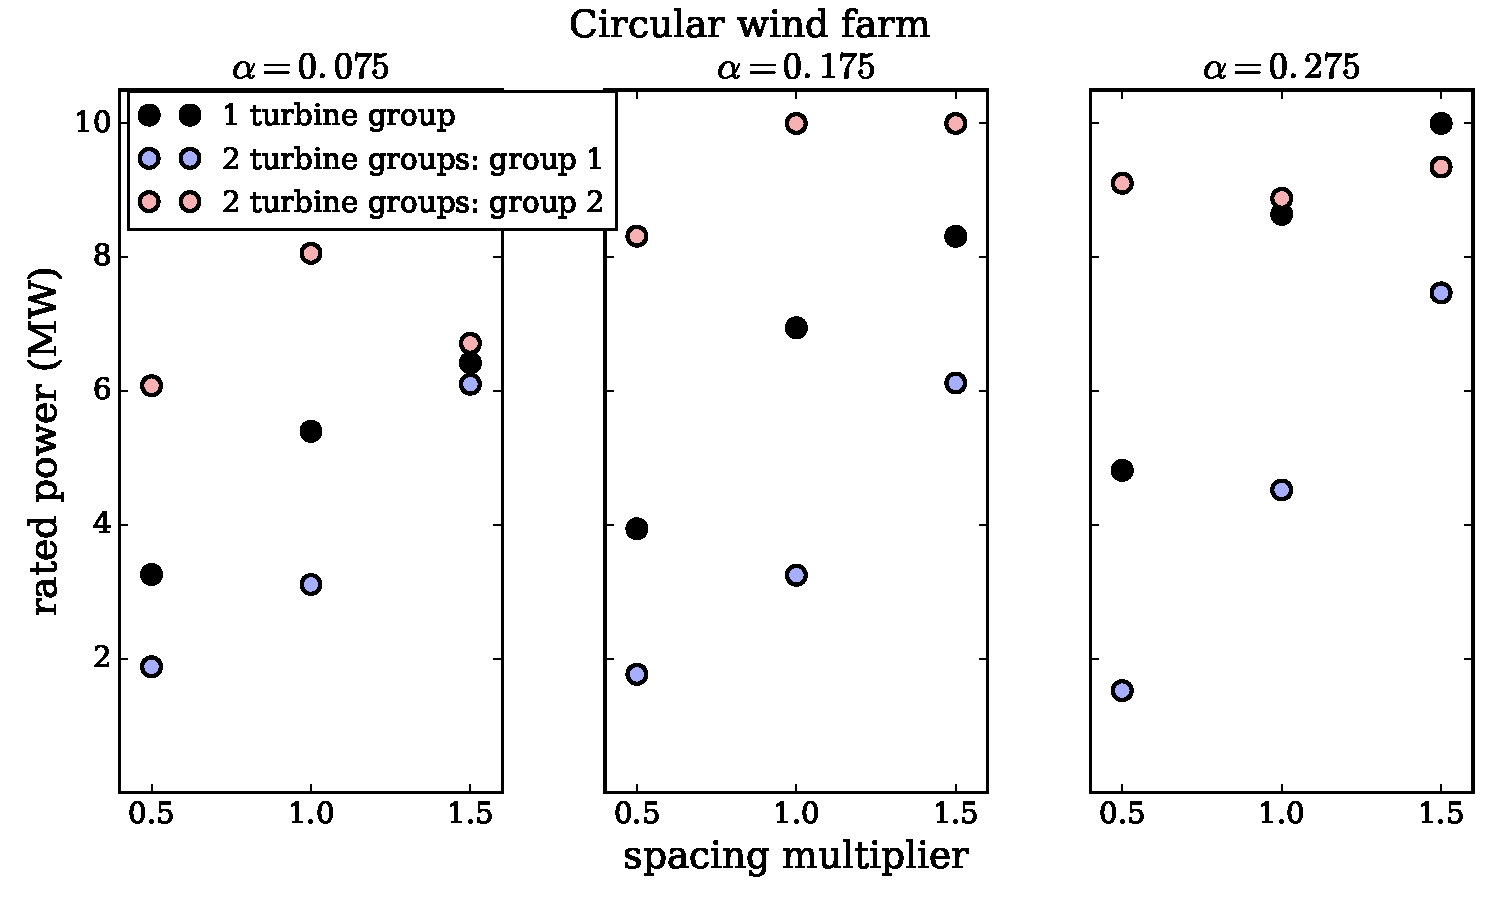
\includegraphics[width=0.8\textwidth]{Figures/circlePowers.pdf}
  \caption{\label{circular_power} The optimal rated powers for the circular wind farm for the optimization runs with coupled layout and turbine design for both uniform wind farm turbine design and with two different turbine design groups. The three subfigures show a different shear exponent, with $\alpha=0.075,0.175,0.275$ from left to right. within each subfigure, the x axis shows different farm spacing multipliers, with $\beta=0.5,1.0,1.5$ from left to right.}
\end{figure}

Table \ref{circular_table} shows how the optimal COE results shown in Fig. \ref{circular_results} compare to the layout optimization with the baseline wind turbine design. These numbers are to compare the relative benefit of performing turbine design with the various scenarios mentioned; they do not indicate a superior wind farm. Take for example two cases, Case A and Case B. Case A is when $\alpha=0.075$ and $\beta=0.5$, for the coupled turbine design and layout optimization with two turbine groups. This Case has an optimal COE 21.6\% lower than the layout-only optimization COE. For Case B, when $\alpha=0.275$ and $\beta=0.5$ for the coupled turbine design with just one height group, the optimal COE is 11.15\% lower than the layout-only optimization case. This does not mean that Case A is better than B (it is not, as seen in Fig. \ref{circular_results}); it simply means that it is able to a achieve a greater COE improvement relative to the layout optimization baseline case. With this in mind, notice that for a spacing multiplier $\beta=0.5$, the relative improvement of two turbine design groups is far superior to coupled design and layout optimization with one turbine group. Also, for $\beta=0.5,1.0$, coupled turbine design and layout optimization is significantly better than the sequential optimization.

\begin{center}
\begin{table}
\caption{The percent COE decrease of the various optimization cases with respect to layout-only optimization performed for the circular wind farm. This table does not show the overall desirability of the optimal wind farm, but the relative improvement of different considerations of turbine design optimization. In the table are shown results for each shear exponent, $\alpha$, as well as each spacing multiplier, $\beta$, in which the smaller spacing multipliers represent farms with turbines that are more closely spaced.}
\label{circular_table}
\begin{tabular}{p{2.5cm} c c c c c c c c c c c}
%\begin{tabularx}{\textwidth}{|X|c|c|c|c|c|c|c|c|c|}
\hline
\multicolumn{10}{c}{\textbf{circular wind farm: percent COE decrease from layout only optimization}}\\
\hline
 & \multicolumn{3}{c}{$\alpha=0.075$} & \multicolumn{4}{c}{$\alpha=0.175$} & \multicolumn{4}{c}{$\alpha=0.275$}\\
\hline
optimization case & $\beta\myeq0.5$ & $\beta\myeq1.0$ & $\beta\myeq1.5$ & & $\beta\myeq0.5$ & $\beta\myeq1.0$ & $\beta\myeq1.5$& &$\beta\myeq0.5$ & $\beta\myeq1.0$ & $\beta\myeq1.5$\\
%\specialrule{.2em}{.1em}{.1em}
sequential & \textcolor{red}{-23.07} & 15.90 & 24.84 & & \textcolor{red}{-15.19}  & 18.13 & 24.37 & & \textcolor{red}{-6.97}  & 22.01 & 26.64\\
%\hline
coupled: 1 group& 12.59  & 22.72  & 27.62  & & 10.24  & 22.88  & 27.87 & & 11.15 & 24.66 & 28.52 \\
%\hline
coupled: 2 groups & 21.60  & 23.88  & 27.54 & & 21.67  & 25.23  &  27.90 & &  22.60 & 26.46  & 28.64\\
\hline
%\end{tabularx}
\end{tabular}
\end{table}
\end{center}











\subsection{Princess Amalia Wind Farm Results}

Figure \ref{amalia_results} shows the COE results for the 60-turbine Princess Amalia wind farm optimizations.  The trends are similar to the smaller, circular wind farm. Coupled turbine design and layout optimization is superior to optimizing each sequentially, especially for the smaller wind farms where the wind speeds are much lower than the free stream. For the farms with closely spaced wind turbines, two different turbine designs in the same farm are significantly better than the farms optimized with a homogeneous turbine design. If the largest wind farms ($\beta=1.5$) benefit from two different turbine design groups, that benefit is negligible. 

\begin{figure}[htbp]
  \centering
  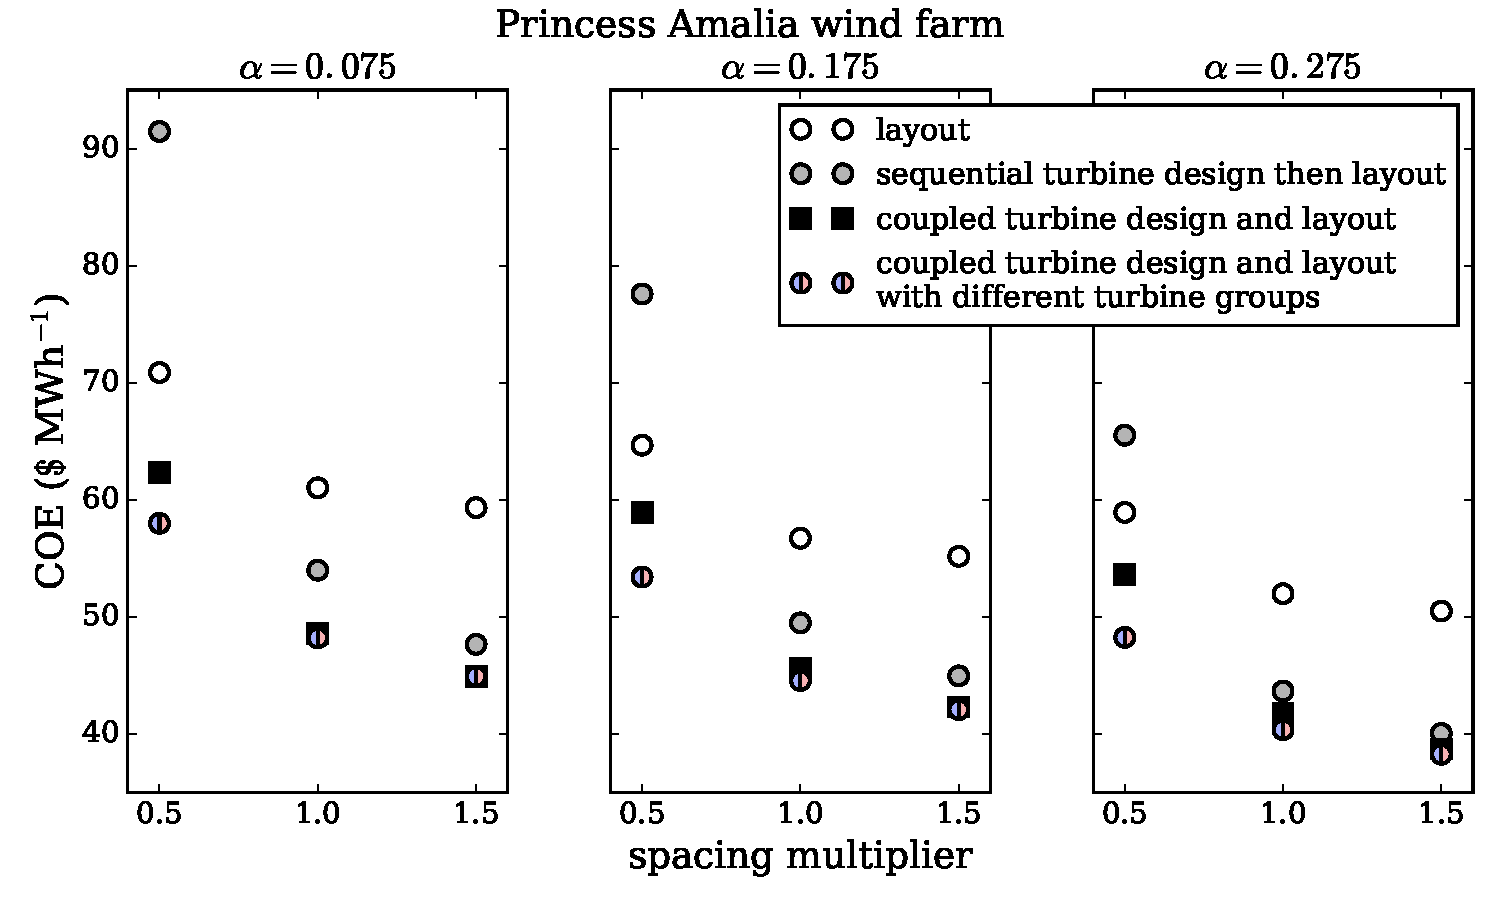
\includegraphics[width=0.8\textwidth]{Figures/amalia_results1.pdf}
  \caption{\label{amalia_results} The optimal COE results for the Princess Amalia wind farm layout with 32 turbines. Each of the subfigures corresponds to optimization runs with a different shear exponent, from left to right $\alpha=0.075,0.175,0.275$. Within each subfigure, the x axis shows the size of the wind farm based on the spacing multiplier, from left to right $\beta=0.5,1.0,1.5$. The different points represent the layout optimization, sequential turbine-design-then-layout optimization, coupled layout-and-turbine-design optimization with homogeneous turbine design throughout the farm, and layout-and-turbine-design optimization with two different turbine design groups.}
\end{figure}

Figures \ref{amalia_turbines_seq}, \ref{amalia_turbines_1},  and \ref{amalia_turbines} show the turbine rotor diameters and hub heights for the various optimization runs,  Fig. \ref{amalia_power} shows the optimal rated powers for the coupled turbine-design-and-layout optimizations, and Table \ref{amalia_table} tabulates the relative benefit of each optimization compared to the layout only optimization. The trends, and reasons behind them, are the same as for the circular wind farm optimizations. We will therefore not repeat this discussion, but will briefly discuss the significant differences between the optimizations of the 32-turbine circular wind farm and those for the 60-turbine Princess Amalia wind farm. The optimal COE values for the Princess Amalia wind farm are slightly lower across the board than the circular wind farm COE values. This is partly because there are more turbines in the Princess Amalia wind farm so a smaller portion of the total cost comes from overhead, but is partly due to the Princess Amalia wind turbines being spaced slightly farther apart than those in the circular wind farms. Another major difference between the optimal COE values of each wind farm is in the optimization case with two turbine design groups. For the Princess Amalia wind farm and a spacing multiplier of 0.5, two turbine groups provides and additional COE decrease of 6.13--9.11\% compared to the wind farm with homogeneous turbine design. This is significant, however it is not as large as the 9.01--11.45\% additional COE decrease in the circular wind farm optimizations for the same spacing multiplier. Again, the main cause of this seems to be that the circular wind farms are slightly closer together than the Princess Amalia wind farms. The conclusion remains the same, wind farms with closely spaced wind turbines greatly benefit from different turbine designs. The last significant difference between the wind farm is that the optimal turbine designs for the Princess Amalia wind farms are slightly smaller than in the circular wind farms. This is due to the different wind roses and speed distributions used to optimized each wind farm. 







%\subsubsection{Sequential Turbine Design then Layout Optimization}

\begin{figure}[htbp]
  \centering
  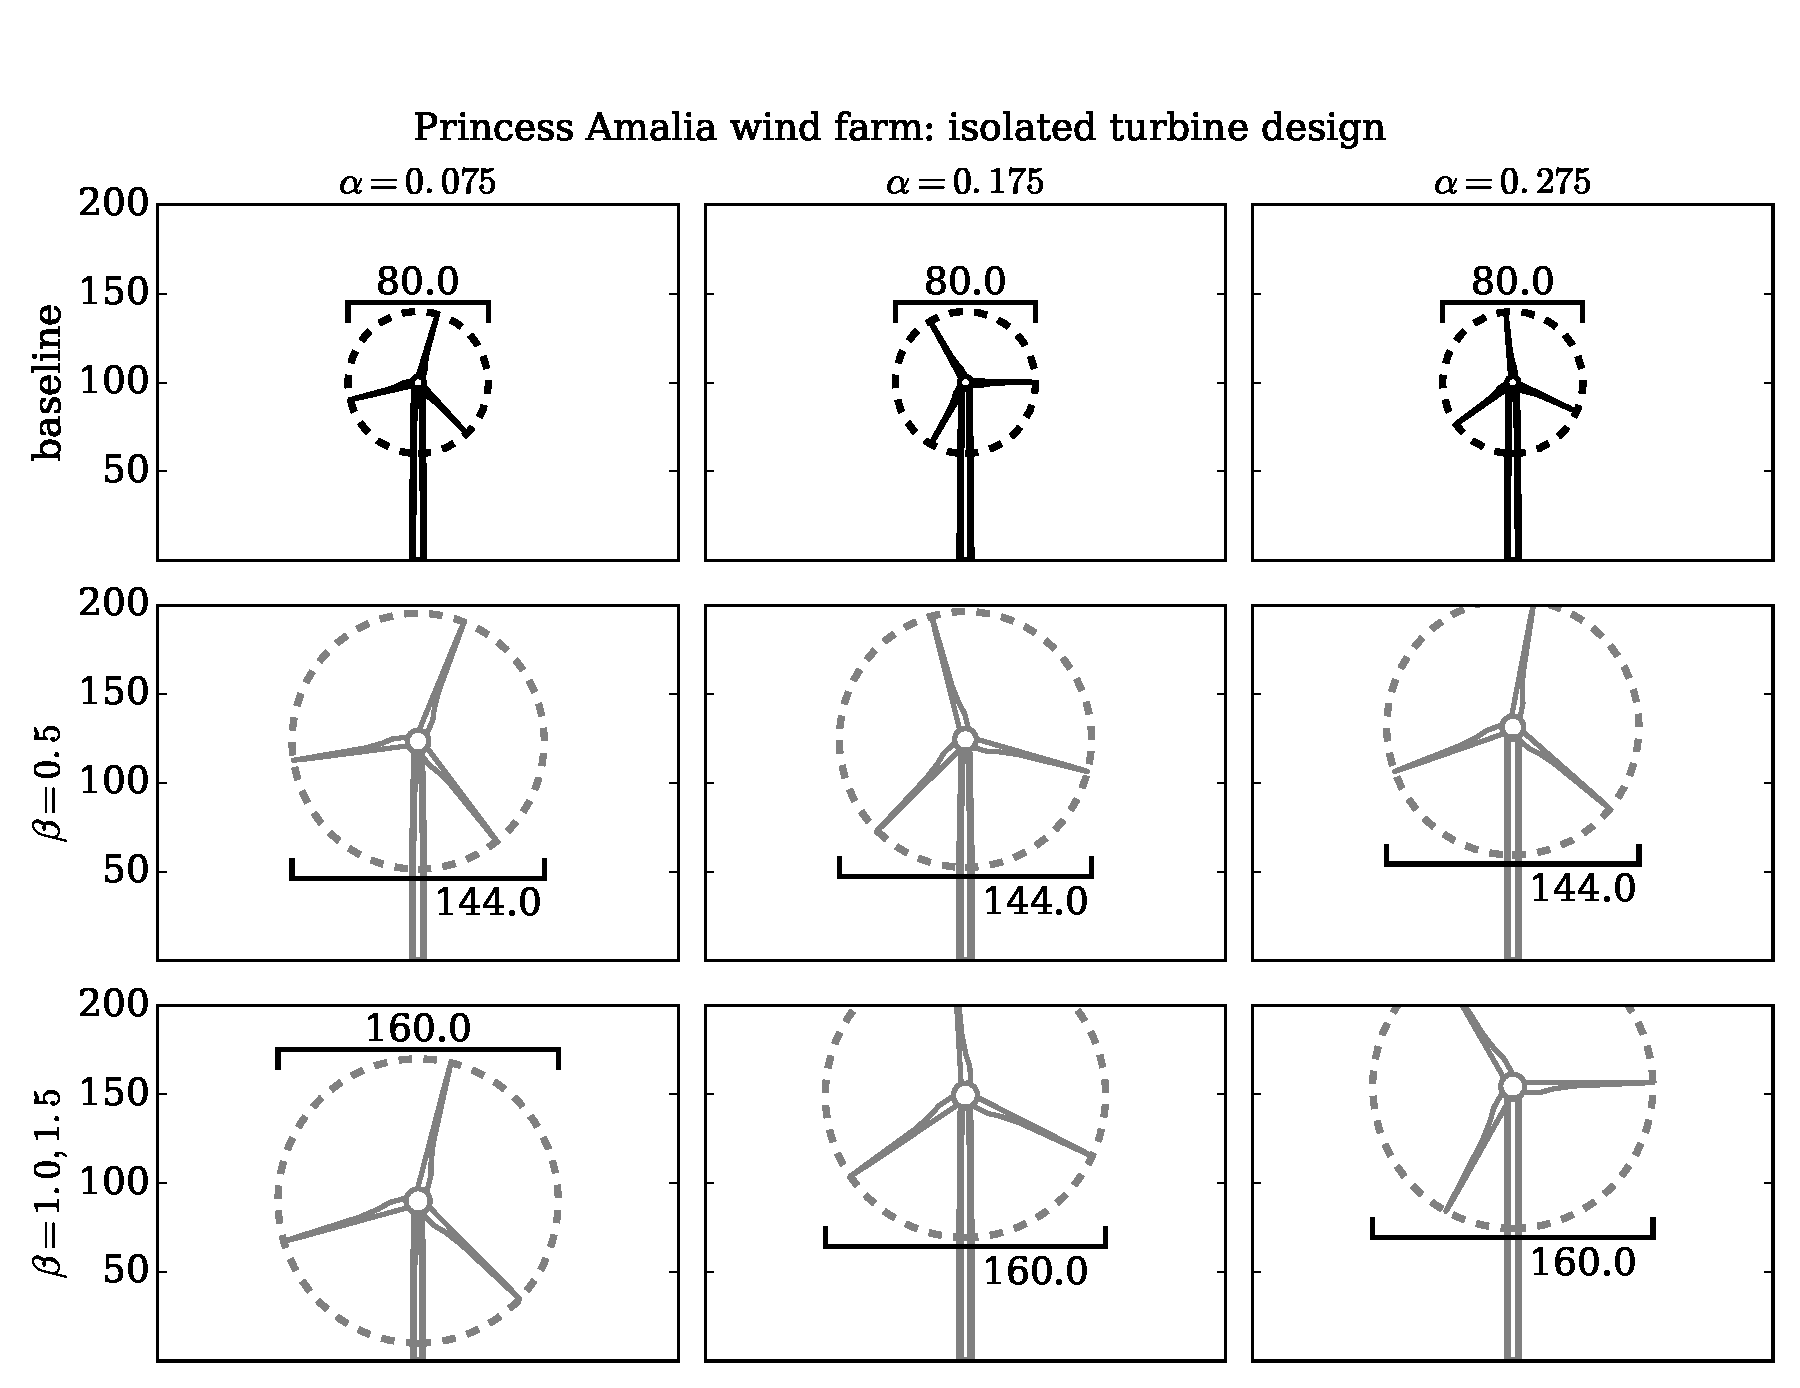
\includegraphics[width=0.8\textwidth]{Figures/turbineSizesAmalia_sequential.pdf}
  \caption{\label{amalia_turbines_seq} The optimal turbine heights and rotor diameters for the isolated turbine design optimization for the Princess Amalia farm wind conditions. These designs were then used in the sequential turbine-design-then-layout optimizations. The columns, from left to right, show the turbines optimized for $\alpha=0.075,0.175$, and $0.275$. The rows, from top to bottom, show the baseline turbine design, the turbine optimized for the small wind farm ($\beta=0.5$), and the turbine designs for the larger wind farms ($\beta=1.0,1.5$)}
\end{figure}




%\subsubsection{Coupled Turbine Design and Layout Optimization}

\begin{figure}[htbp]
  \centering
  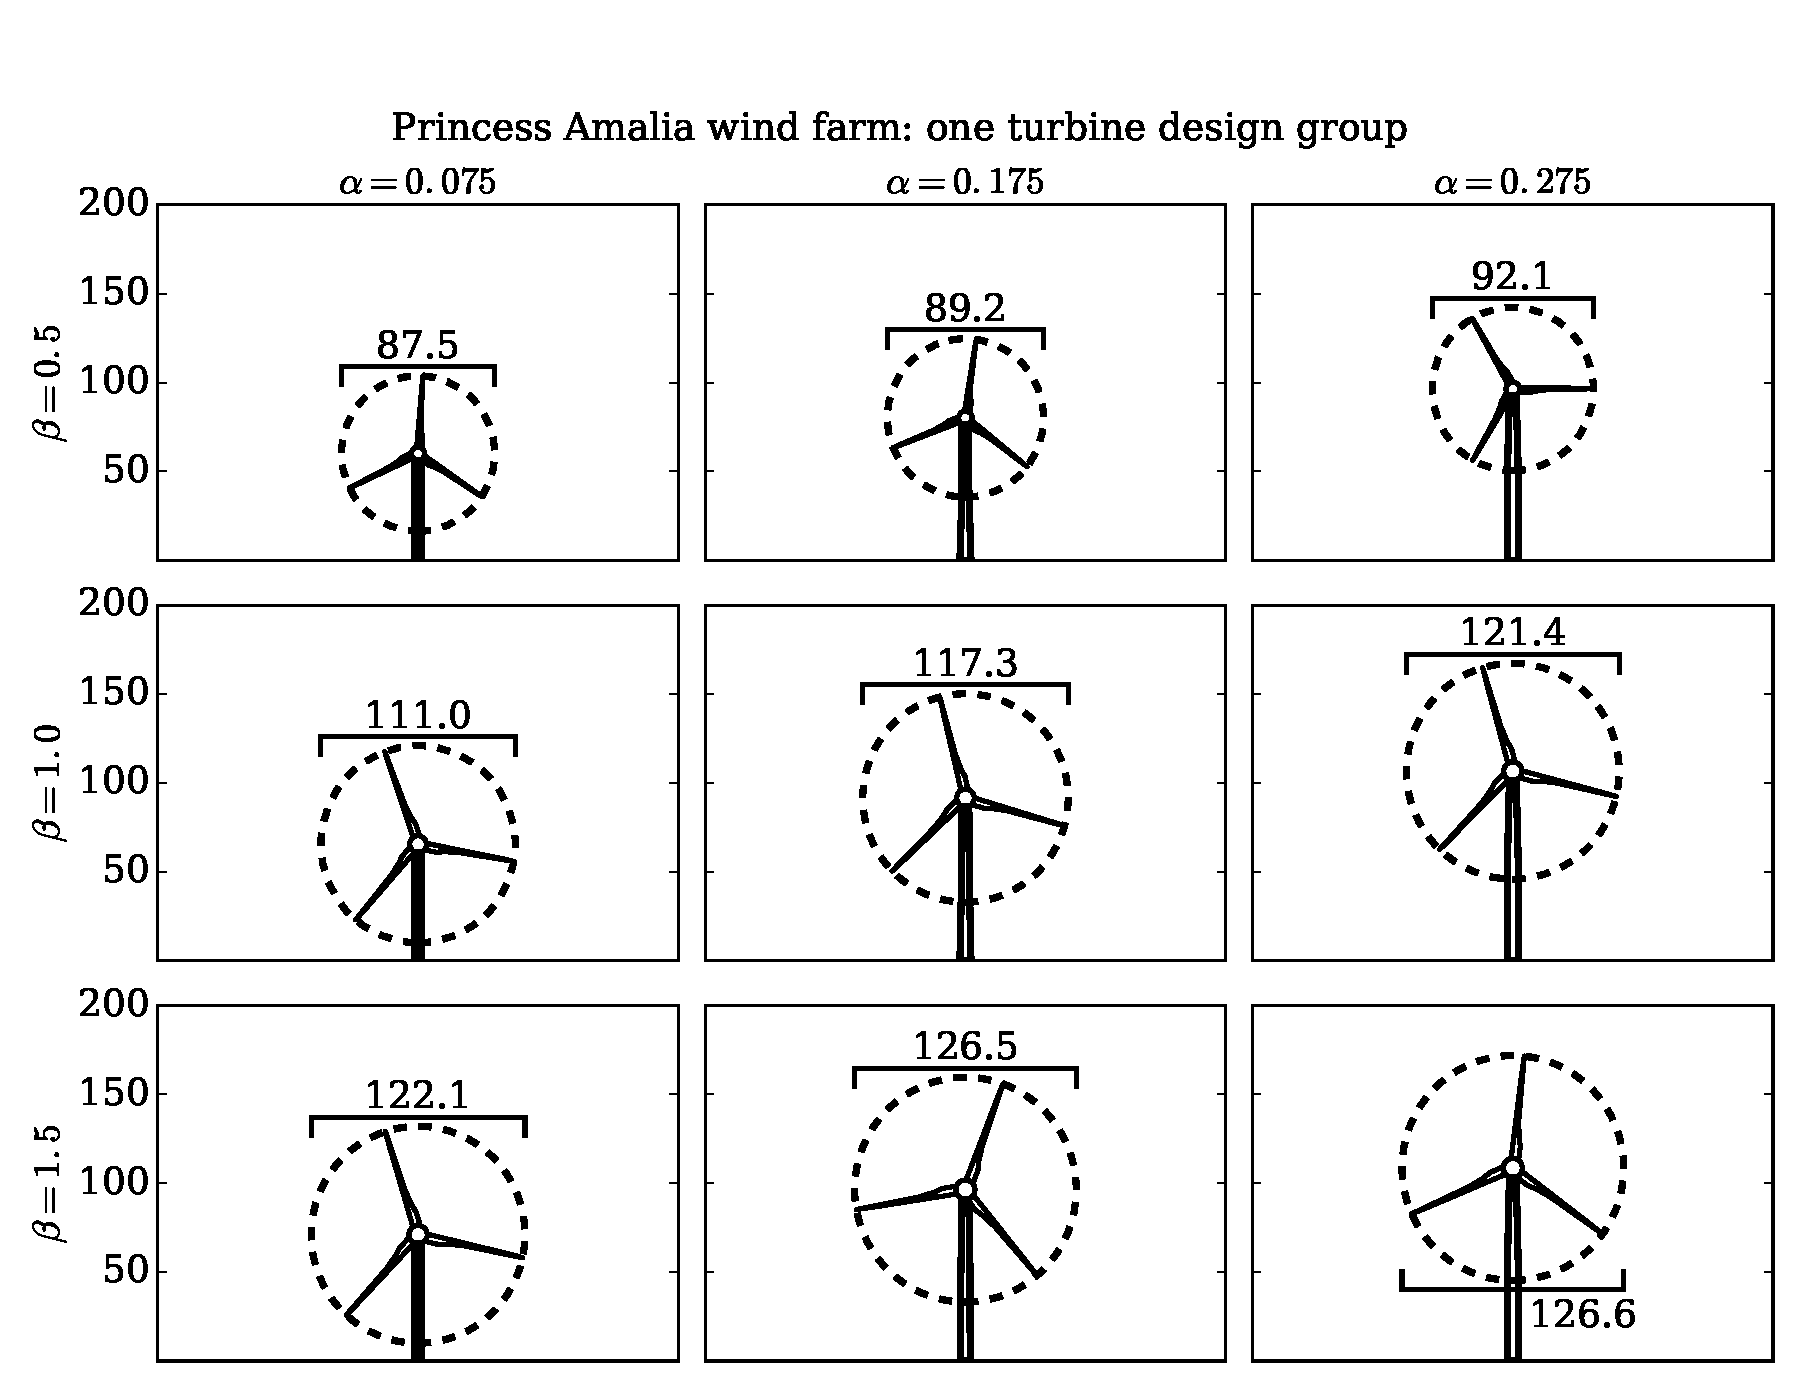
\includegraphics[trim={0.5cm 0.3cm 0.3cm 1.75cm},clip,width=0.8\textwidth]{Figures/turbineSizesAmalia_1.pdf}
  \caption{\label{amalia_turbines_1} The optimal turbine heights and rotor diameters for the optimization runs with coupled layout and turbine design with homogeneous turbine design throughout the circular wind farm. Each column shows a different shear exponent, with $\alpha=0.075,0.175,0.275$ from left to right. Each row shows a different farm spacing multiplier, with $\beta=0.5,1.0,1.5$ from top to bottom.}
\end{figure}



%\subsubsection{Coupled Turbine Design and Layout Optimization with Two Turbine Groups}

\begin{figure}[htbp]
  \centering
  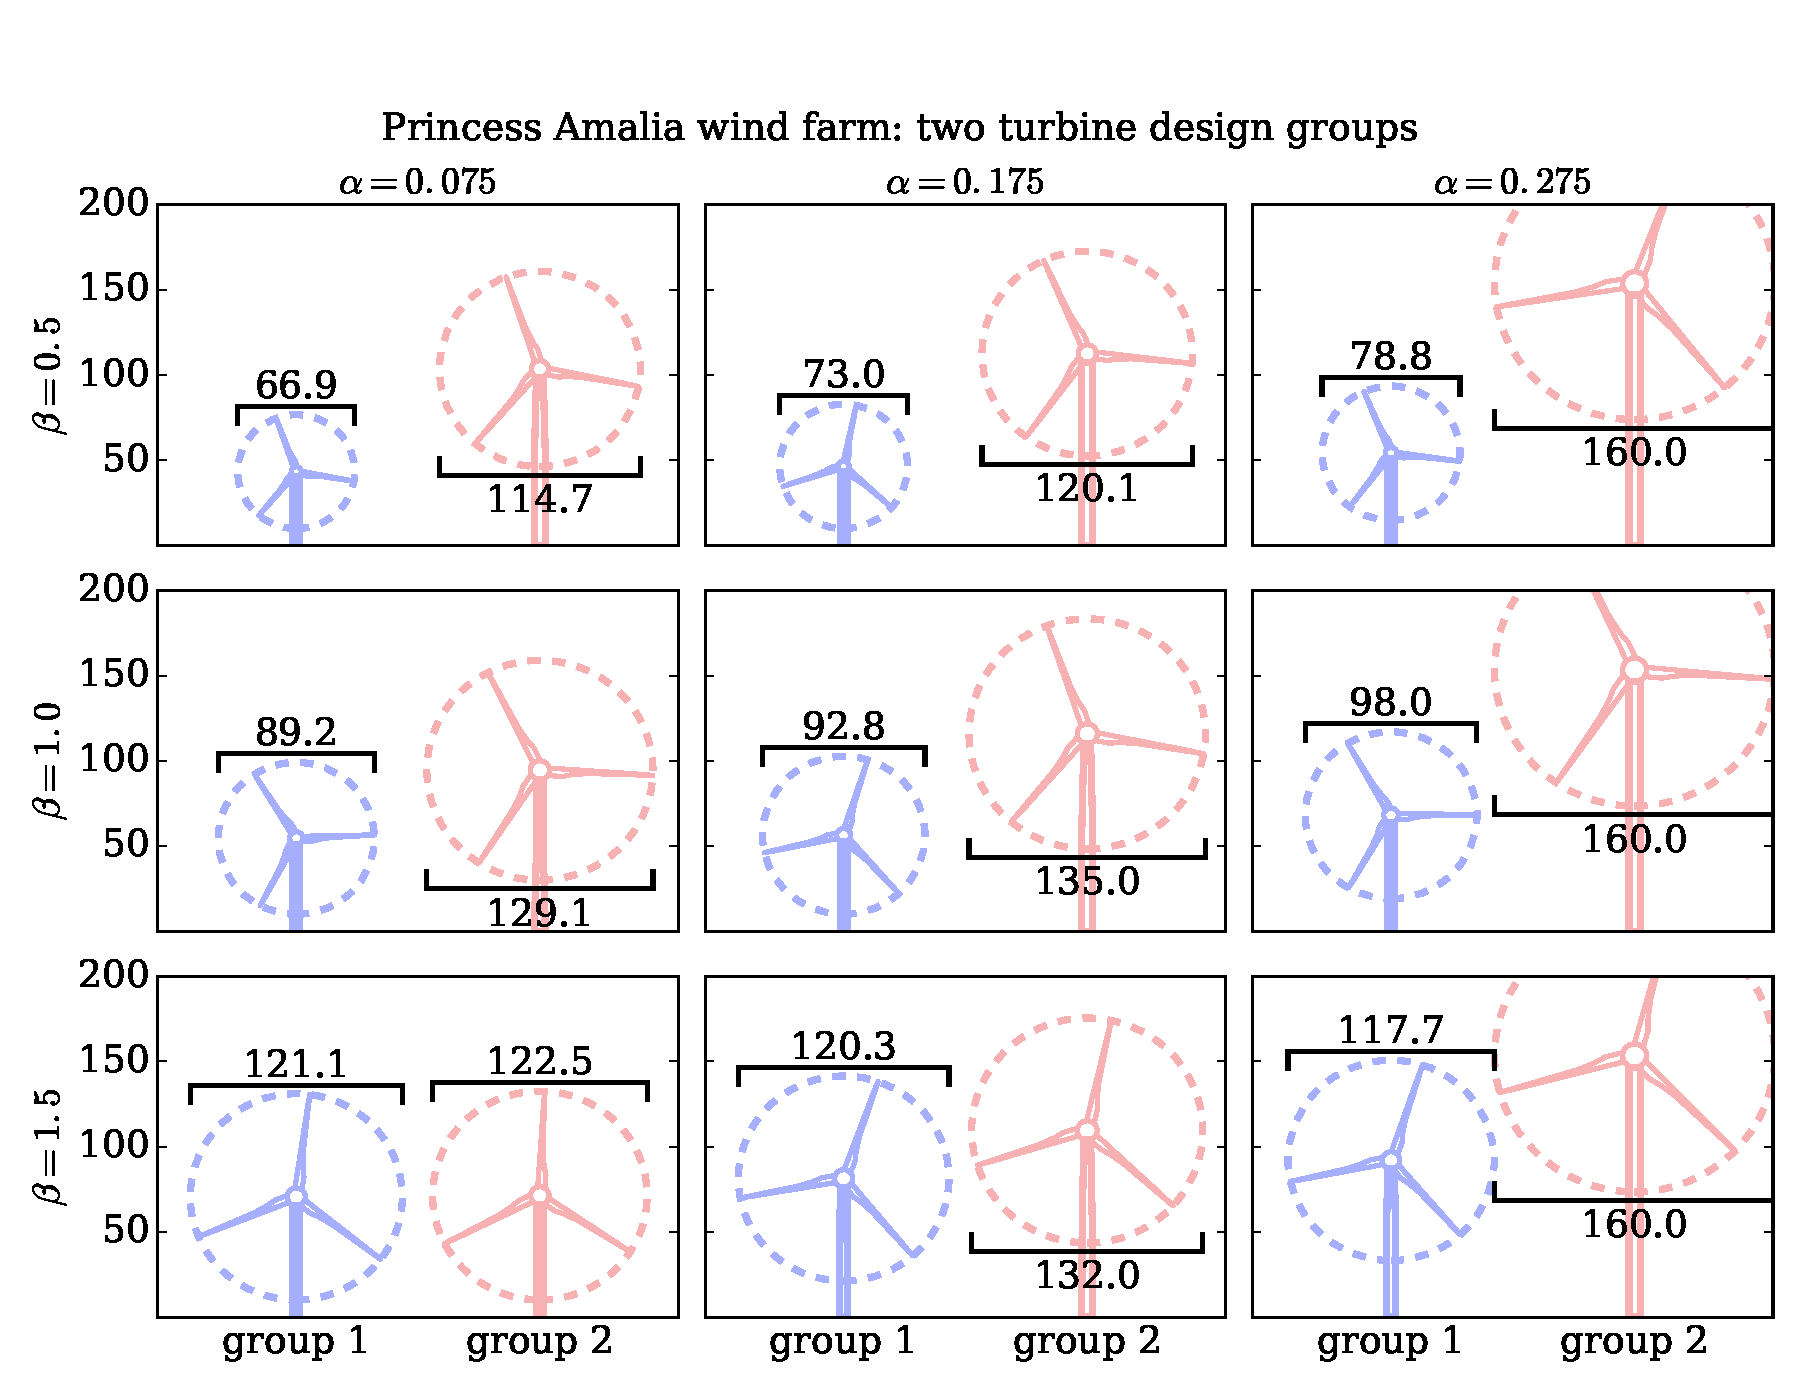
\includegraphics[trim={0.5cm 0.3cm 0.3cm 1.75cm},clip,width=0.8\textwidth]{Figures/turbineSizesAmalia_2.pdf}
  \caption{\label{amalia_turbines} The optimal turbine heights and rotor diameters for the optimization runs with coupled layout and turbine design with two different turbine design groups for the circular wind farm. Each column shows a different shear exponent, with $\alpha=0.075,0.175,0.275$ from left to right. Each row shows a different farm spacing multiplier, with $\beta=0.5,1.0,1.5$ from top to bottom.}
\end{figure}


\begin{figure}[htbp]
  \centering
  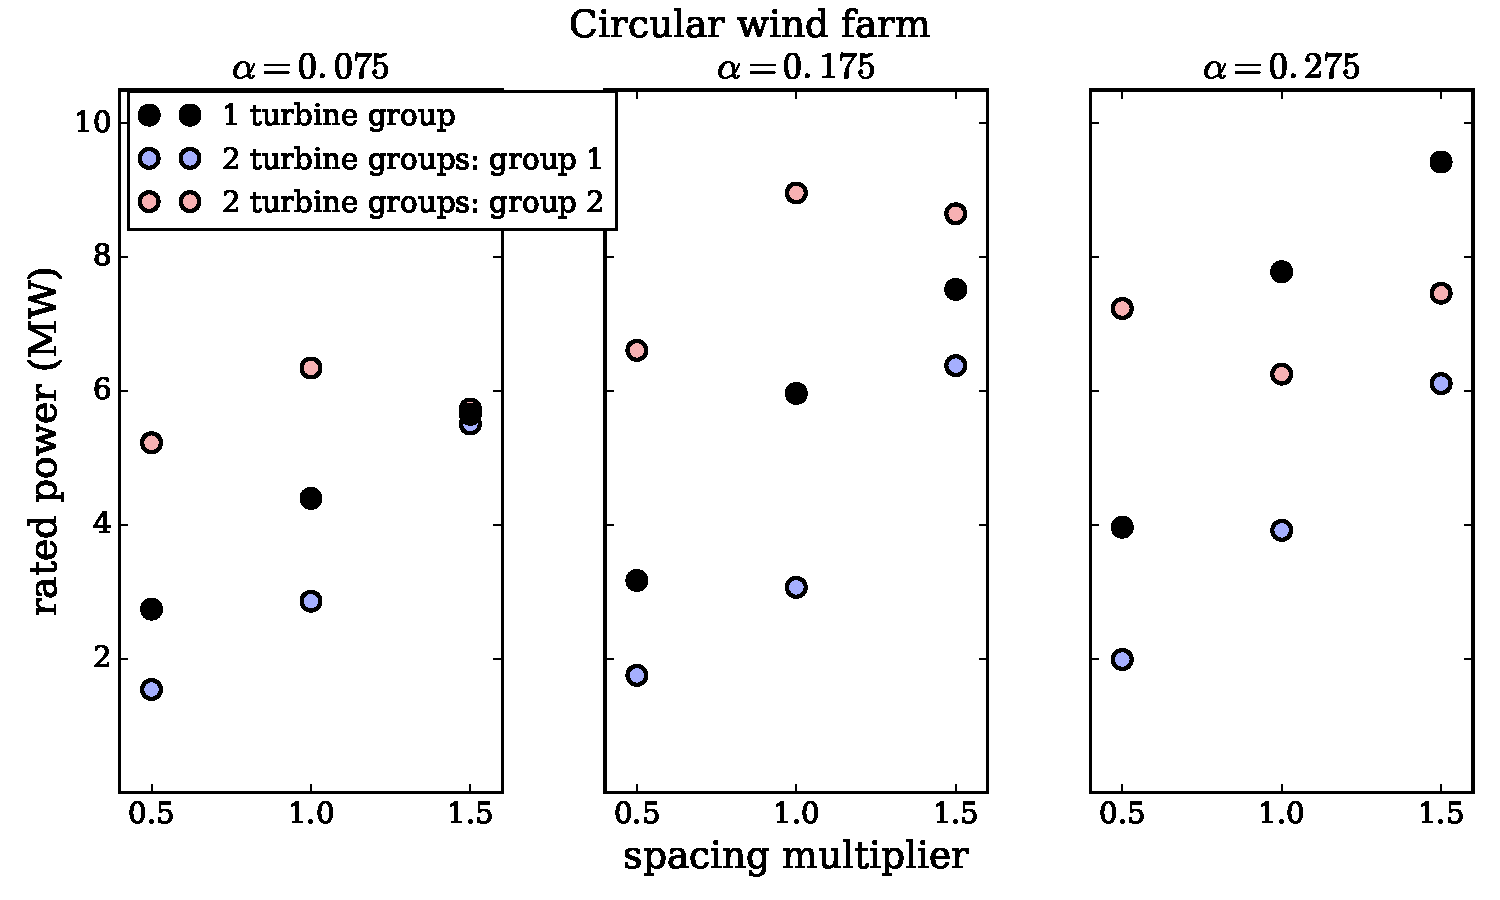
\includegraphics[width=0.8\textwidth]{Figures/amaliaPowers.pdf}
  \caption{\label{amalia_power} The optimal rated powers for the Princess Amalia wind farm for the optimization runs with coupled layout and turbine design for both uniform wind farm turbine design and with two different turbine design groups. The three subfigures show a different shear exponent, with $\alpha=0.075,0.175,0.275$ from left to right. within each subfigure, the x axis shows different farm spacing multipliers, with $\beta=0.5,1.0,1.5$ from left to right.}
\end{figure}




\begin{center}
\begin{table}
\caption{The percent COE decrease of the various optimization cases with respect to layout-only optimization performed for the Princess Amalia wind farm. This table does not show the overall desirability of the optimal wind farm, but the relative improvement of different considerations of turbine design optimization. In the table are shown results for each shear exponent, $\alpha$, as well as each spacing multiplier, $\beta$, in which the smaller spacing multipliers represent farms with turbines that are more closely spaced.}
\label{amalia_table}
\begin{tabular}{p{2.5cm} c c c c c c c c c c c}
%\begin{tabularx}{\textwidth}{|X|c|c|c|c|c|c|c|c|c|}
\hline
\multicolumn{10}{c}{\textbf{Princess Amalia wind farm: percent COE decrease from layout only optimization}}\\
\hline
 & \multicolumn{3}{c}{$\alpha=0.075$} & \multicolumn{4}{c}{$\alpha=0.175$} & \multicolumn{4}{c}{$\alpha=0.275$}\\
\hline
optimization case & $\beta\myeq0.5$ & $\beta\myeq1.0$ & $\beta\myeq1.5$ & & $\beta\myeq0.5$ & $\beta\myeq1.0$ & $\beta\myeq1.5$& &$\beta\myeq0.5$ & $\beta\myeq1.0$ & $\beta\myeq1.5$\\
%\specialrule{.2em}{.1em}{.1em}
sequential & \textcolor{red}{-29.06} & 11.54 & 19.70 & & \textcolor{red}{-19.98}  & 12.74 & 18.52 & & \textcolor{red}{-11.19}  & 16.02 & 20.70\\
%\hline
coupled: 1 group& 12.05  & 20.45  & 24.34  & & 8.94  & 19.61  & 23.32 & & 9.00 & 19.66 & 23.33 \\
%\hline
coupled: 2 groups & 18.18  & 21.01  & 24.30 & & 17.41  & 21.45  &  23.74 & &  18.11 & 22.37  & 24.24\\
\hline
%\end{tabularx}
\end{tabular}
\end{table}
\end{center}


% \subsection{Princess Amalia Wind Farm Optimization}

% % Figure \ref{amalia_results} shows the optimal COE results for the Princess Amalia wind farm. As expected, the higher wind speed from high wind shear results in a lower optimal COE. Additionally, the widely spaced wind turbines indicated by the larger spacing multipliers also result in lower COE. 
% % For every shear exponent and spacing multiplier there is a small decrease in optimal COE from the baseline wind farm to when layout optimization has occurred. The largest benefit from layout optimization occurs for the smallest wind farms with COE decreases from 2.39-2.48\%, while for spacing multiplier of 1.0 and 1.5, the COE decrease is negligible, from 0.26-0.62\%. In these cases where turbines are farther apart, there is already minimal wake interference between wind turbines, so layout optimization does not provide a significant benefit. The very small COE decrease, even for the spacing multiplier of 0.5, indicates that the baseline layout is already very good and that this is a well designed wind farm layout for the turbines that are used. 

% % Optimizing the turbine design along with the farm layout provides significant COE decrease compared to baseline, and compared to the layout only optimization. First we will discuss the turbine design optimization in which there is homogeneous design for all turbines in the wind farm. For a spacing multiplier of 0.5, there is a COE decrease of 11.24-14.46\% across all of the wind shears. For the more widely spaced wind farms, the COE decrease is even greater at 20.19-24.97\%. 
% % %
% % This is incredible! An additional 10-25\% decrease in COE from a wind farm with quasi-optimal turbine layout is amazing. Designing the wind turbines appropriately wind conditions they will experience in the wind farm environment can amount to worthwhile gains in energy production and cost reduction.
% % %
% % For the optimization cases that we ran, the larger wind farms benefited more from turbine design optimization than the smaller farm. For the larger wind farms, turbine wake interactions are not as detrimental because the slow moving wakes have begun to recover much of the momentum that was lost. Therefore, a turbine design with a large rotor and high rated power is cost effective. For the smaller wind farm, where the average wind speed is lower throughout the farm because of turbine wakes, a smaller turbine and lower rated power, closer to the original baseline values, is optimal.
% % %
% % % These results indicate the importance of designing turbines for the wind conditions and the specific wind farm where they will operate. Not only are the freestream wind conditions important, but the atmospheric boundary layer and the turbine spacing in the wind farm. Optimizing turbine design finds the hub height, rotor diameter, and rated power that best captures the energy in the wind farm for the lowest cost.

% % Now we will discuss the additional benefit that comes from two different turbine designs used throughout the wind farm. For the tightly spaced wind farms (spacing multiplier of 0.5), there is additional COE decrease in the wind farms with two different turbine groups. Across all the shear exponents, there is an additional 5.95-8.68\% COE decrease from baseline compared to the farm with homogeneous turbine design. In these tightly packed wind farms, there is significant wake interaction between the turbines. In such cases, having different turbine designs reduces the wake interaction with different hub heights and rotor diameters, as shown in the top row of Figure \ref{amalia_turbines}. For the spacing multiplier of 0.5, one turbine group is very short and small, while the other is taller and large. Rather than have all the turbines have a large swept area and be tall to reach the fast moving freestream air, it is more beneficial to have one small turbine group which avoids the wakes of the tall turbines, and doesn't produce wakes that will interfere much with the taller group. 
% % When the turbines are close to each other as they are with a spacing multiplier of 0.5, a lot of power is lost through wake interactions among turbines. Because of the tight spacing, moving turbines in the horizontal plane through layout optimization is not as successful in avoiding the wakes of other turbines. Thus in this case, the different heights and rotor diameters are very successful in reducing COE in a wind farm because they allow turbines to avoid wakes vertically as well as in the horizontal plane. 
% % The turbine rating of each group is also optimized to produce as much energy as each group is capable, but not be over-rated such that turbine costs rise without an associated increase in energy production. In the larger wind farms, there is still a small benefit to having the two different turbine groups, but not nearly as pronounced as the small wind farm. In the middle and bottom rows of Figure \ref{amalia_turbines} are the optimal sizes of the different turbine groups. The difference between the rotor diameters of each turbine group decreases as the distance between the turbines increases. For the largest spacing multiplier, the turbines in each group are almost exactly the same. When the turbines are farther apart, the wake interactions are not as detrimental, making it more beneficial to have the turbine groups be more similar to each other, and to the wind farm optimized with homogeneous turbine design.


% % Figure \ref{amalia_power} shows the optimal rated powers of each turbine group for each optimization. Note that the larger rated powers correspond to the taller, larger wind turbines from Figure \ref{amalia_turbines}. There is no need for the smaller and shorter turbines to have a very high rated power if the energy they can produce is limited by their size.
% % Table \ref{tab:amalia} shows the percent decrease in COE for each optimization case compared to the baseline. Note that the higher percent decrease does not mean a more desirable wind farm. The lowest overall COE is achieved in wind farms with a high wind shear and turbines spaced far apart. This table shows how much better a wind farm can be with turbine design and layout optimization, compared to a sub-optimal wind farm.


% % Figures \ref{amalia_turbines} and \ref{amalia_power} show the optimal turbine hub heights, rotor diameters, and rated powers for the wind farms with two different turbine groups. For the spacing multiplier of 0.5, there is a large difference between the hub heights and rotor diameters of each turbine group. When the turbines are close to each other as they are with a spacing multiplier of 0.5, a lot of power is lost through wake interactions among turbines. Because of the tight spacing, moving turbines in the horizontal plane through layout optimization is not as successful in avoiding the wakes of other turbines. Thus in this case, the different heights and rotor diameters are very successful in reducing COE in a wind farm because they allow turbines to avoid wakes vertically as well as in the horizontal plane. 


% \begin{figure}[htbp]
%   \centering
%   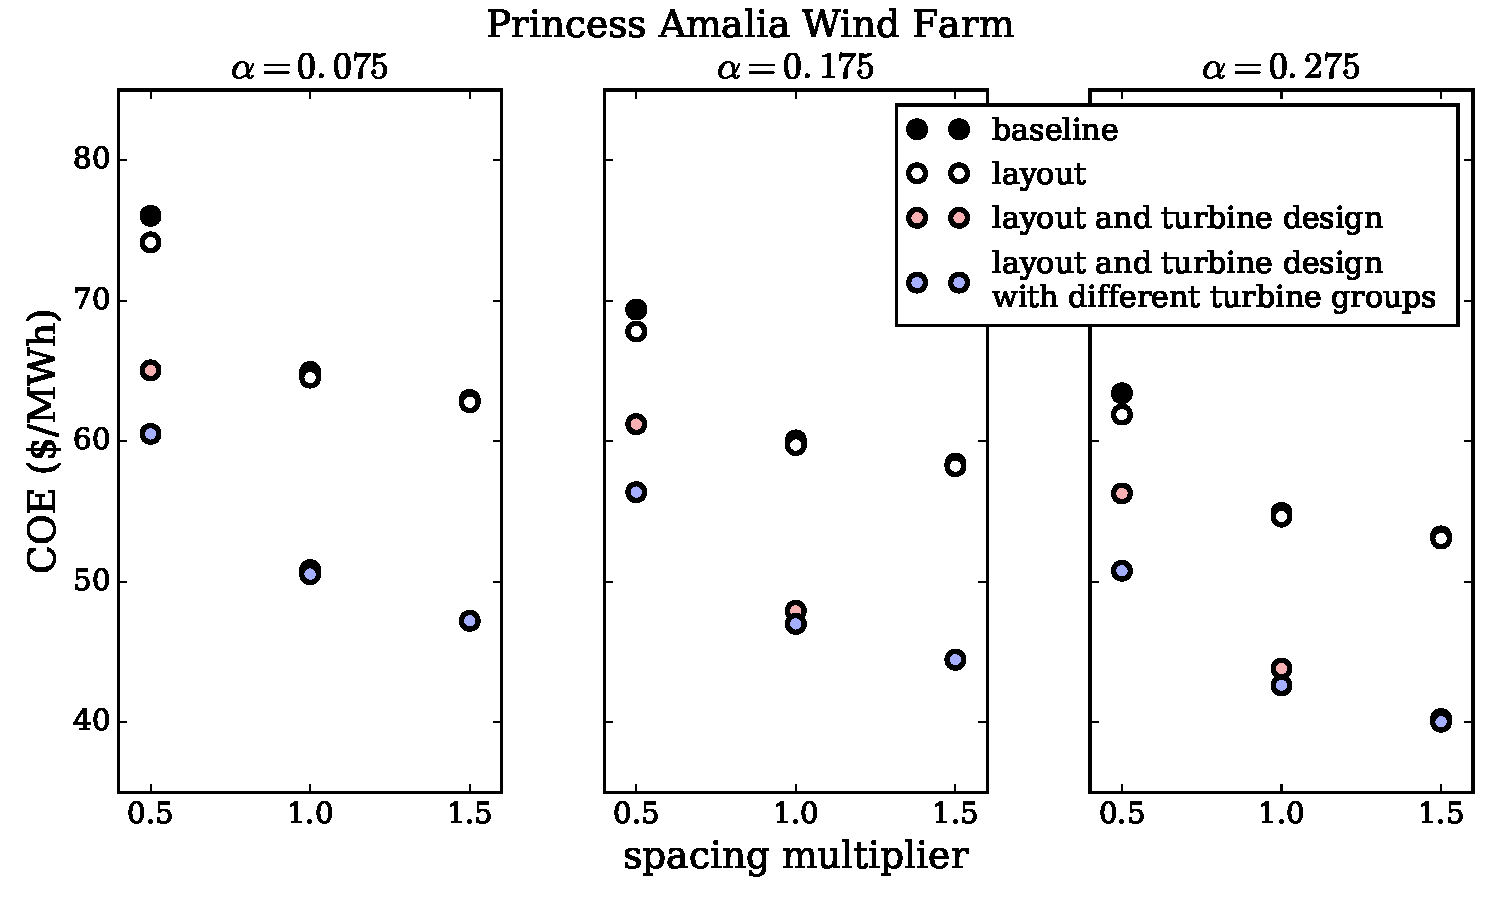
\includegraphics[width=\textwidth]{Figures/amalia_results.pdf}
%   \caption{\label{amalia_results} The optimal COE results for the Princess Amalia wind farm layout with 60 turbines. Each of the subfigures corresponds to optimization runs with a different shear exponent, from right to left $\alpha=0.075,0.175,0.275$. With in each subfigure, the x axis shows the size of the wind farm through the spacing multiplier, from right to left $\beta=0.5,1.0,1.5$. The different points represent the baseline, layout optimization, layout and turbine design optimization with homogeneous turbine design throughout the farm, and layout and turbine design optimization with two different turbine design groups.}
% \end{figure}

% \begin{center}
% \captionof{table}{}\label{tab:amalia}
% \begin{tabularx}{\textwidth}{|X|c|c|c|c|c|c|c|c|c|}
% \hline
% \multicolumn{10}{|c|}{\textbf{Princess Amalia: Percent COE Decrease from Baseline}}\\
% \hline
%  & \multicolumn{3}{c|}{$\alpha=0.075$} & \multicolumn{3}{c}{$\alpha=0.175$} & \multicolumn{3}{|c|}{$\alpha=0.275$}\\
% \hline
% optimization case & $\beta\myeq0.5$ & $\beta\myeq1.0$ & $\beta\myeq1.5$ & $\beta\myeq0.5$ & $\beta\myeq1.0$ & $\beta\myeq1.5$& $\beta\myeq0.5$ & $\beta\myeq1.0$ & $\beta\myeq1.5$\\
% \specialrule{.2em}{.1em}{.1em}
% layout & 2.48 & 0.62 & 0.26 & 2.25  & 0.55  & 0.30  & 2.39  & 0.48  & 0.27\\
% \hline
% coupled turbine design & 14.46  & 21.72  & 24.97  & 11.76  &  20.21 &  23.90 & 11.24  &  20.19 & 24.42\\
% \hline
% coupled turbine design: 2 groups & 20.41  & 22.17  & 24.98  & 18.74  & 21.75  & 23.88  & 19.92  &  22.34 & 24.79\\
% \hline
% \end{tabularx}
% \end{center}

% % The optimal rated power is low for the short, small turbines that won't produce as much energy, and larger for the taller, larger rotors that are capable of producing much more energy.

% \begin{figure}[htbp]
%   \centering
%   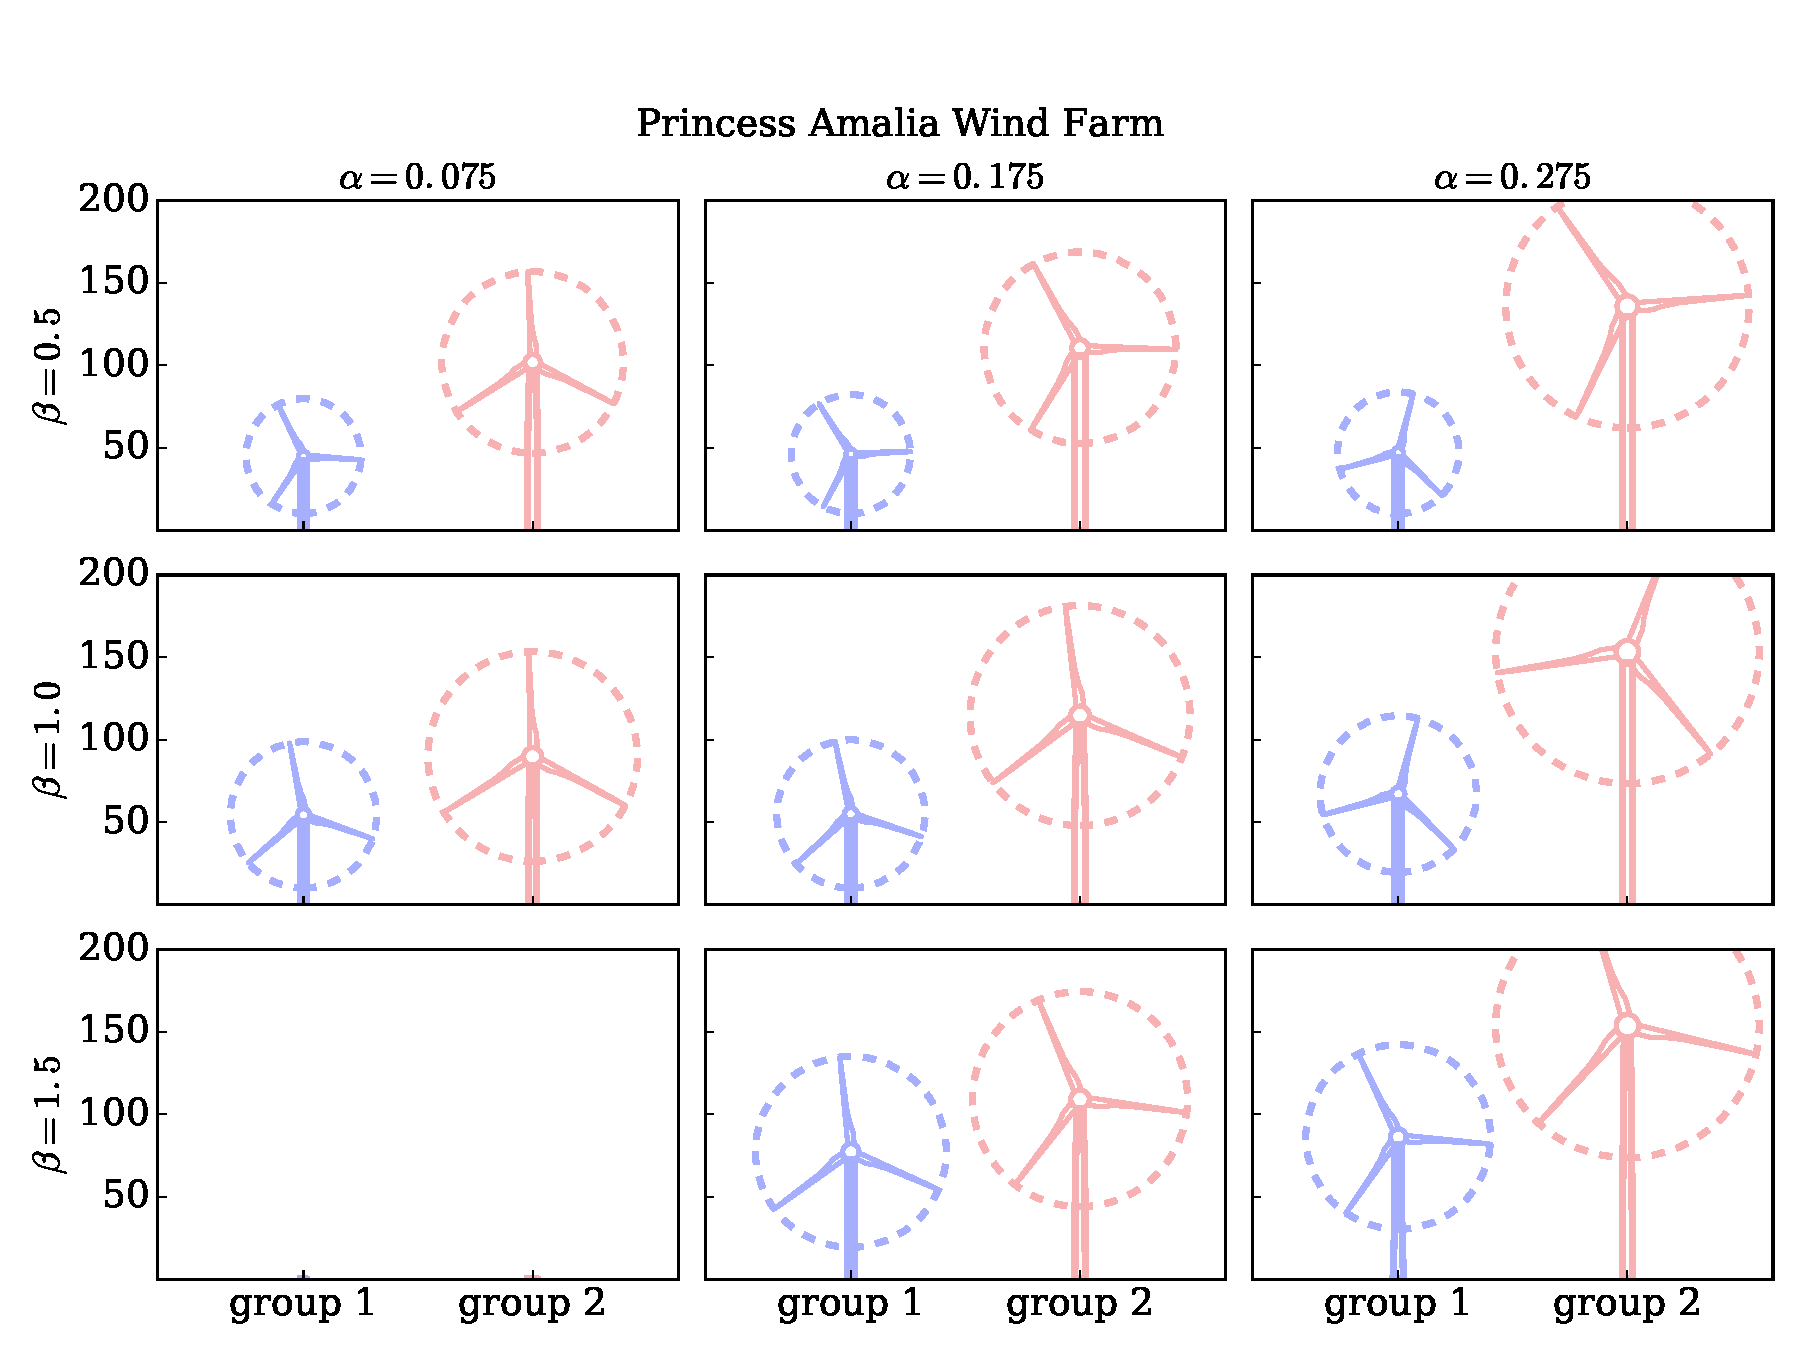
\includegraphics[trim={0.5cm 0.3cm 0.3cm 1.75cm},clip,width=\textwidth]{Figures/turbineSizesAmalia.pdf}
%   \caption{\label{amalia_turbines} The optimal turbine heights and rotor diameters for the optimization runs with coupled layout and turbine design with two different turbine design groups for the Princess Amalia wind farm. Each column shows a different shear exponent, with $\alpha=0.075,0.175,0.275$ from left to right. Each row shows a different farm spacing multiplier, with $\beta=0.5,1.0,1.5$ from top to bottom.}
% \end{figure}

% \begin{figure}[htbp]
%   \centering
%   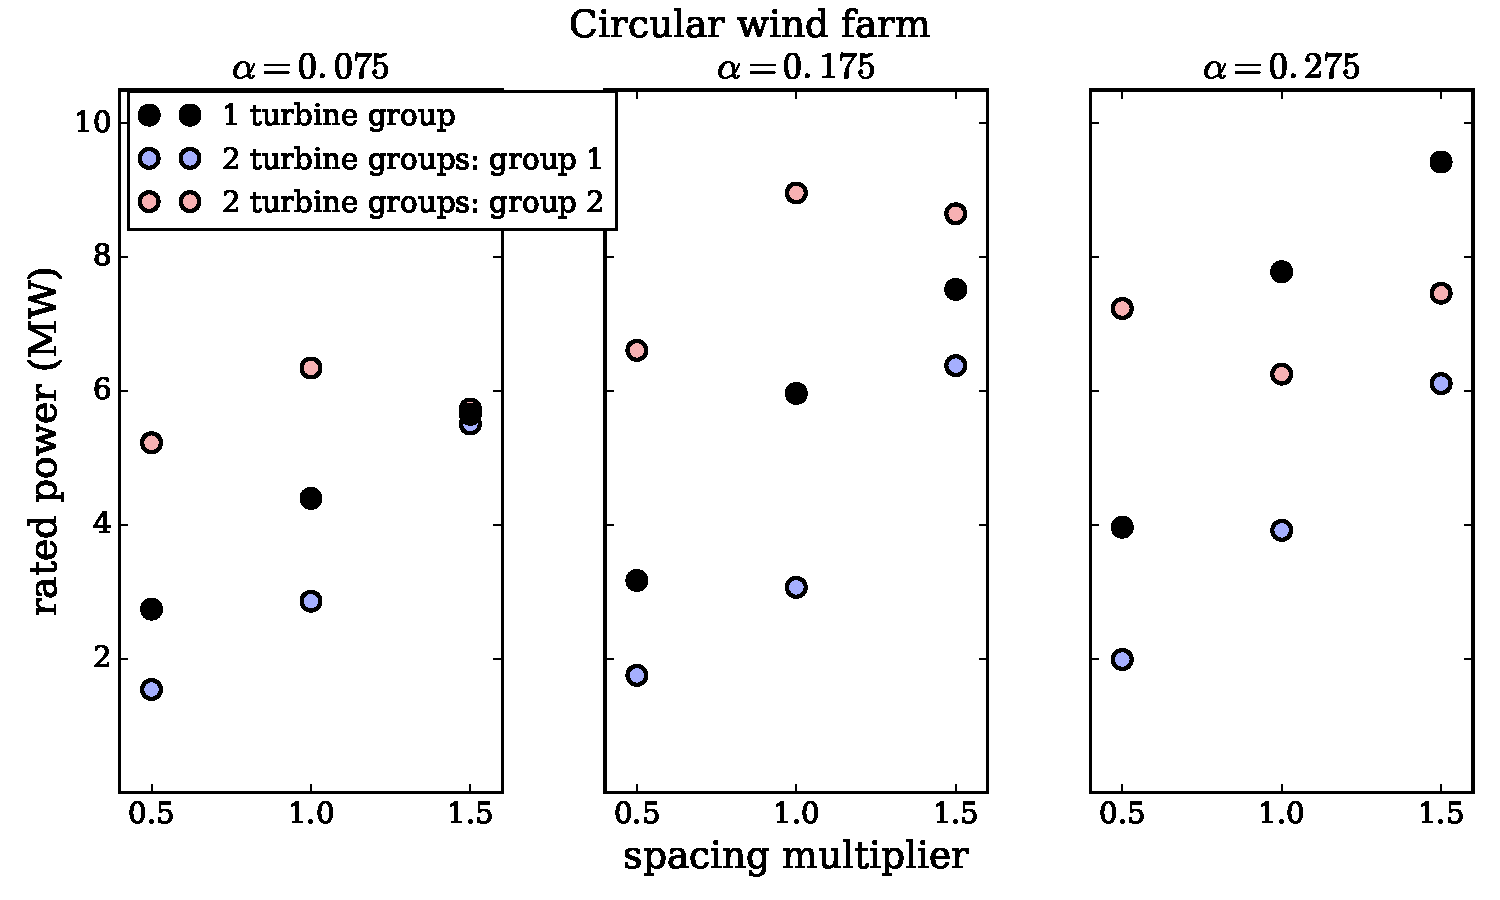
\includegraphics[trim={0.9cm 0cm 1.5cm 0cm},clip,width=\textwidth]{Figures/amaliaPowers.pdf}
%   \caption{\label{amalia_power} The optimal rated powers of each group for the optimization runs with coupled layout and turbine design with two different turbine design groups for the Princess Amalia wind farm. The three subfigures show a different shear exponent, with $\alpha=0.075,0.175,0.275$ from left to right. within each subfigure, the x axis shows different farm spacing multipliers, with $\beta=0.5,1.0,1.5$ from left to right.}
% \end{figure}





\newcommand\myeq{\mkern1.5mu{=}\mkern1.5mu}


In this section we will discuss the optimization results of both wind farms, the apparent benefit of coupled turbine layout and design optimization, as well as the benefit of heterogeneous turbine design in a wind farm.
We first present results from the 32-turbine circular wind farm optimizations and then compare to the 60-turbine Princess Amalia wind farm optimizations. 
%First, we present the circular wind farm optimal results for each wind shear exponent and spacing multiplier combination. 
%Each combination of shear exponent and spacing multiplier has four points, representing a layout optimization performed with the baseline turbine design, a turbine design optimized in isolation followed by layout optimization, coupled layout and homogeneous turbine design optimization, and finally coupled layout and turbine design optimization with two different turbine groups. 
%Finally, we show the optimal COE results of the Princess Amalia wind farm optimizations and compare them to those from the circular wind farm.
% Figures \ref{circular_turbines} and \ref{amalia_turbines} show the turbine heights and rotor diameters in the optimization cases with two different turbine groups. Figures \ref{circular_power} and \ref{amalia_power} show the optimal power rating of each turbine group in the optimization cases with two different height groups. 



\subsection{Circular Wind Farm}

Figure \ref{circular_results} shows the optimal COE results for the circular wind farm. As shown in the legends, the white points represent a layout-only optimization with the baseline turbine design, the gray indicate a sequential-turbine-design-then-layout optimization, the black points show a coupled-turbine-design-and-layout optimization, and the half blue and pink points represent a coupled design and layout optimization with two turbine groups.  As expected, the general trends for all optimizations run show that the higher wind speed from high wind shear results in a lower, superior optimal COE. Additionally, the widely spaced wind turbines indicated by the larger spacing multipliers also result in lower COE due to less wake interaction between turbines. We will discuss each of these optimizations in detail below.


\begin{figure}[htbp]
  \centering
  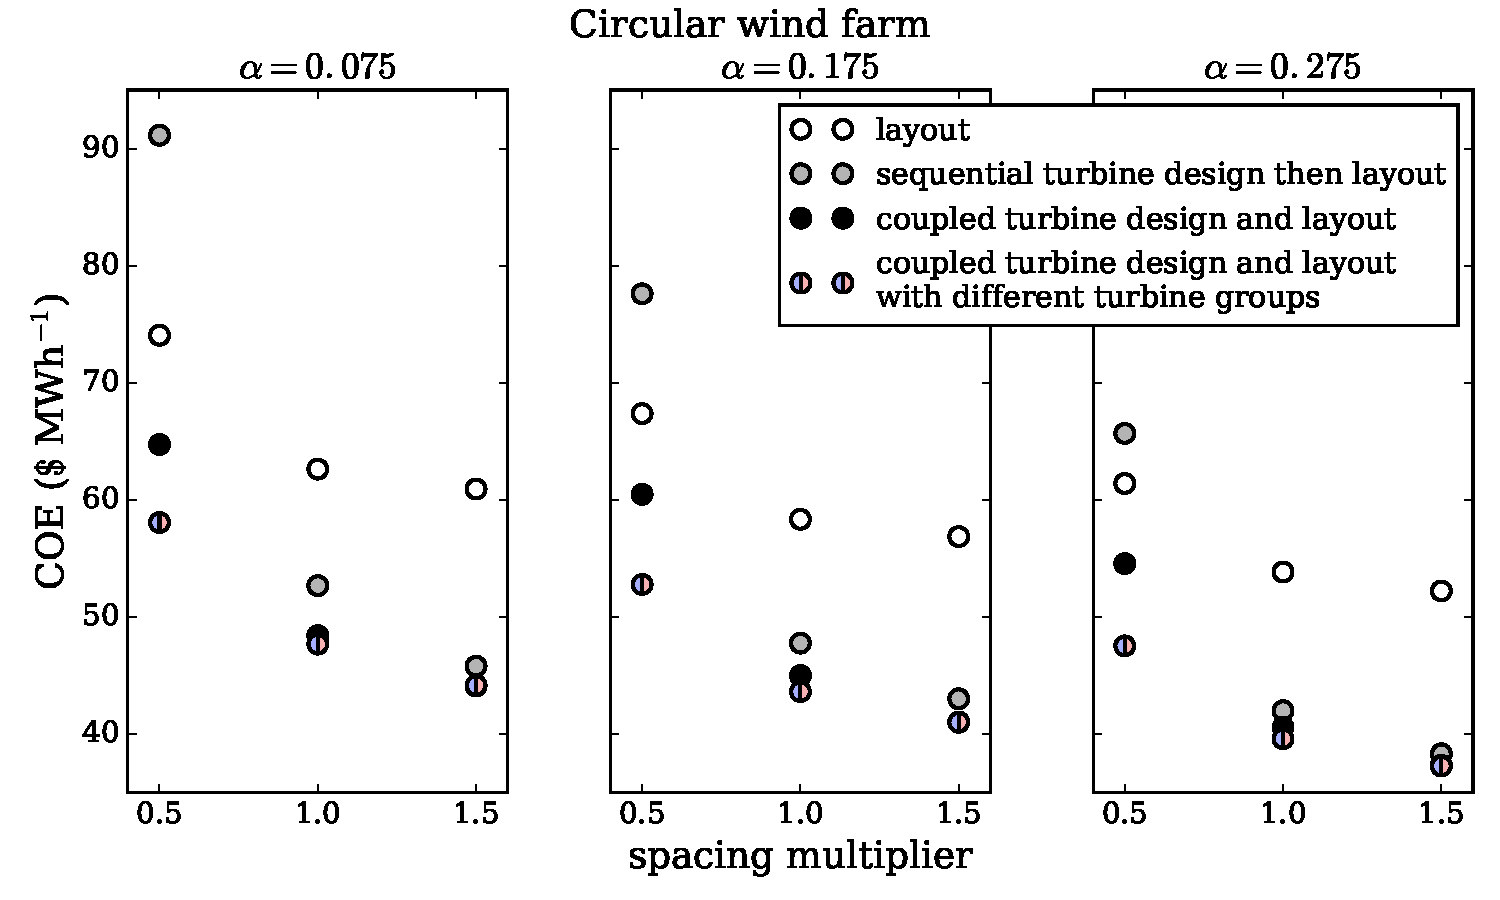
\includegraphics[width=0.7\textwidth]{Figures/circular_results1.pdf}
  \caption{\label{circular_results} The optimal COE results for the circular wind farm layout with 32 turbines. Each of the subfigures corresponds to optimization runs with a different shear exponent, from left to right $\alpha=0.075,0.175,0.275$. Within each subfigure, the x axis shows the size of the wind farm based on the spacing multiplier, from left to right $\beta=0.5,1.0,1.5$. The different points represent the layout optimization, sequential turbine-design-then-layout optimization, coupled layout-and-turbine-design optimization with homogeneous turbine design throughout the farm, and layout-and-turbine-design optimization with two different turbine design groups.}
\end{figure}



\subsubsection{Circular Wind Farm: Sequential Turbine Design then Layout Optimization}
The gray dots in Fig. \ref{circular_results} show the optimal COE results for a sequential optimization. First, a turbine was designed for minimal COE in isolation with the free stream wind conditions. This turbine design was then used in the wind farm where the layout was optimized. 
The rotor diameter was constrained such that the turbine spacing constraints would be satisfied in the baseline farm where the turbine would be installed. This was only applicable for the smallest wind farms, where $\beta=0.5$. 
For each shear exponent, the optimal turbine design was the maximum rotor diameter and turbine rating allowed by the optimizer.
%: 160 meters and 10 megawatts. 
%The optimal height increased with the shear exponent: 90 meters, 147 meters, and 155 meters for the shear exponents of 0.075, 0.175, and 0.275, respectively.
Figure \ref{circular_turbines_seq} shows the optimal isolated turbine designs for each shear exponent and spacing multiplier, as well as the baseline turbine design. Because these turbines are optimized in isolation, the designs for $\beta=1.0,1.5$ are the same. The only affect the spacing multiplier has on the design is a possible maximum rotor diameter (as in the case of $\beta=0.5$).
When these optimized turbine designs are used in each wind farm instead of the baseline turbine design, there is a large COE improvement for the spacing multipliers of $\beta=1.0, 1.5$. For $\beta=1.0$, COE decreases 15.9--22.0\% compared to an optimized wind farm with the baseline turbine design. For $\beta=1.5$ the COE decrease is even larger, 24.8--26.6\% across all shear exponents. 
%For the smallest wind farm, $\beta=0.5$, the turbine design optimized in isolation results in an infeasible farm layout. The rotor diameter is so large and the farm area so small that no layout is possible where the turbine spacing constraints are satisfied. However, even when the turbine spacing constraints were removed, this sequential turbine-design-then-layout optimization resulted in a worse COE for shear exponents of $\alpha=0.075,0.175$ compared to the layout-only optimization, and only a slightly better COE (2.3\%) for $\alpha=0.275$. 
For the smallest wind farm, $\beta=0.5$, the turbine design optimized in isolation results in an extremely inefficient wind farm. When in the wind farm environment, exposed to much lower average wind speeds, this design results in a COE that is much worse than the baseline turbine design. The expense from a bigger and taller turbine, coupled with the strong wake interactions among turbines that are so closely spaced means that for this wind farm, optimizing the turbine in isolation actually decreases the wind farm performance. 


\begin{figure}[htbp]
  \centering
  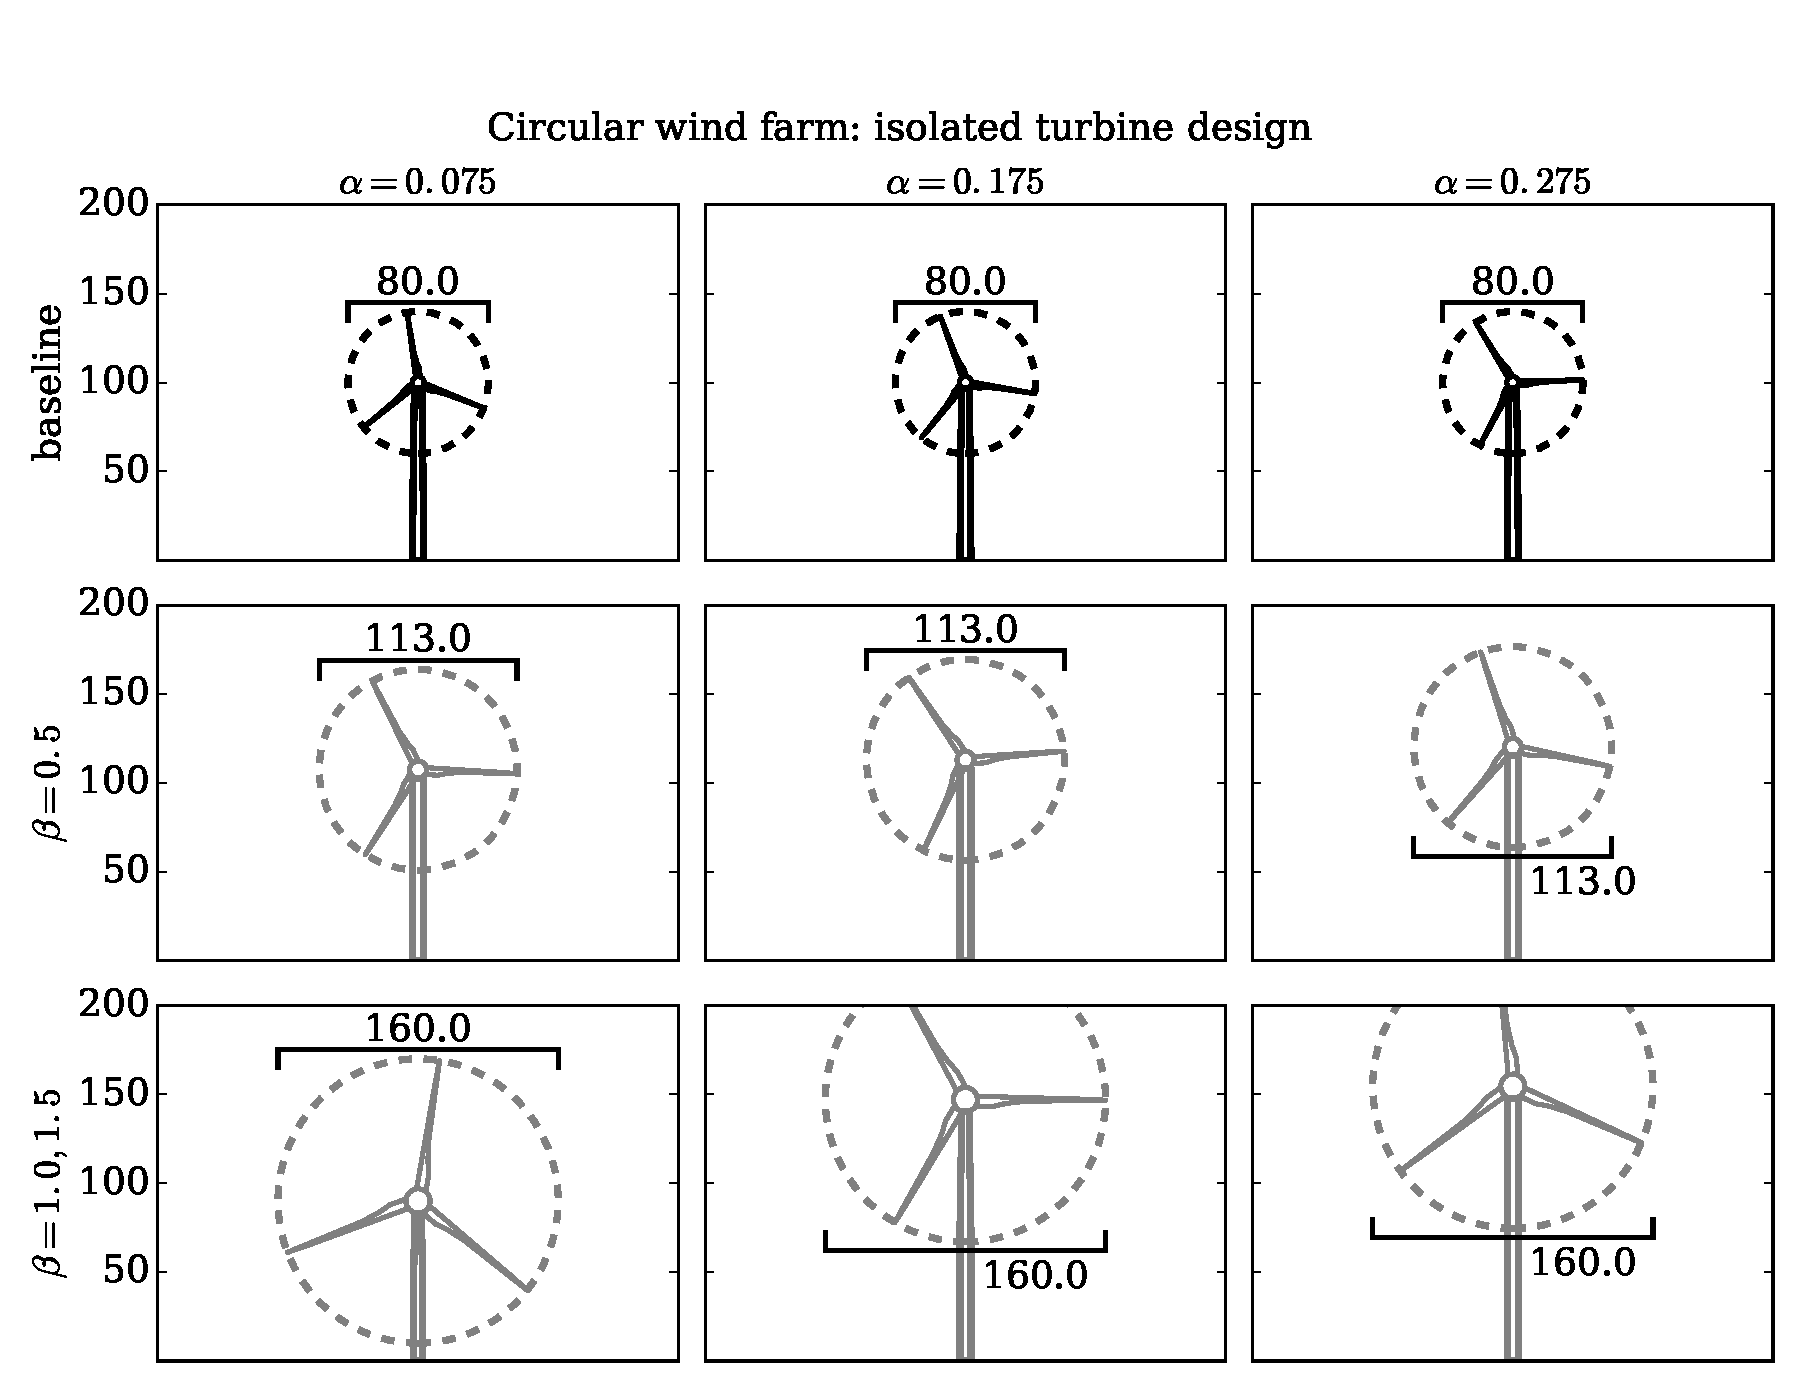
\includegraphics[trim={0.5cm 0.3cm 0.3cm 2.75cm},clip,width=0.7\textwidth]{Figures/turbineSizesCircular_sequential.pdf}
  \caption{\label{circular_turbines_seq} The optimal turbine heights and rotor diameters for the isolated turbine design optimization for the circular farm wind conditions. These designs were then used in the sequential turbine-design-then-layout optimizations. The columns, from left to right, show the turbines optimized for $\alpha=0.075,0.175$, and $0.275$. The rows, from top to bottom, show the baseline turbine design, the turbine optimized for the small wind farm ($\beta=0.5$), and the turbine designs for the larger wind farms ($\beta=1.0,1.5$)}
\end{figure}



\subsubsection{Circular Wind Farm: Coupled Turbine Design and Layout Optimization}
Next we will discuss the optimization results of the coupled turbine-design-and-layout optimizations, represented by the black dots in Fig. \ref{circular_results}. For every shear exponent and spacing multiplier, there is a large benefit to performing the coupled turbine-design-and-layout optimization compared to the layout-only optimization with the baseline turbine design. Additionally, and more importantly, the coupled optimization results in appreciably lower COE than the sequential design-then-layout optimization. Obviously for a spacing multiplier of $\beta=0.5$, the coupled optimization is far superior to the sequential in that it results in a feasible wind farm. For the spacing multiplier of $\beta=1.0$, 
% which results in feasible wind farms for the sequential optimizations as well as the coupled optimizations, 
compared to the sequential optimizations, coupled optimization results in an additional 6.82\%, 4.75\%, and 2.65\% COE improvement from layout only optimization for shear exponents $\alpha=0.075, 0.175,$ and $0.275$, respectively. For the largest wind farm, $\beta=1.5$, the coupled optimization results in an additional 2.78\%, 3.50\%, and 1.88\% COE improvement compared to the sequential case. 

There are several conclusions we can make from both the sequential and coupled turbine design and layout optimizations. First, and most apparent, optimizing turbine design results in a much better wind farm than a farm in which the turbines are selected arbitrarily or a priori. Second, and more importantly, optimizing turbine design coupled with the turbine layout is significantly better than optimizing the turbine design for the free stream wind conditions alone. In a wind farm, turbines rarely experience the free stream wind conditions as they are often waked by the other turbines in the farm. Therefore, the optimal turbine design is based on on average slower wind speeds than the free stream wind. This results in turbines with smaller hub heights, rotor diameters, and rated powers. 
%
One could conceivably optimize the turbine design for some wind speed slower than the free stream and closer to the average speed in the wind farm, which would likely be better than optimizing the turbine design for the free stream wind speed. However, the average wind speed in a farm is dependent on the turbine layout, making it difficult to choose the correct speed for which to design the turbines. Thus, is important to couple the turbine design and layout optimization for a superior wind farm. 

Figure \ref{circular_turbines_1} shows the optimal rotor diameters and hub heights for the coupled turbine design and layout optimizations. For a spacing multiplier $\beta=0.5$, the turbines are very close together and in general are heavily waked. Thus to satisfy spacing constraints and because the average wind speed is very low, the optimal rotor diameter is small: about 90 meters. When the turbines are spaced farther apart, shown for the larger spacing multipliers, the optimal rotor diameter is much larger: closer to 120--130 meters. In these farms, wake interactions are not as severe, meaning that the extra power production from larger rotors is worth the extra turbine capital cost. Also notice the trend of the optimal turbine height with wind shear exponent. For a low wind shear exponent, $\alpha=0.075$, the wind speed does not drastically change with height (see Fig. \ref{shear_profile}). Therefore, for this wind condition it is desireable to have short hub heights with a lower turbine capital cost. For the higher shear exponents, $\alpha=0.175,0.275$, the wind speed increases much more with height (See Fig. \ref{shear_profile}). In these cases, for every spacing multiplier, the extra cost of building the taller turbines is made up for in the additional power produced from the high wind speeds. Note that a larger rotor diameter reduces the relative spacing between turbines in the farm, as the original spacing was based on a diameter of 80 meters.

\begin{figure}[htbp]
  \centering
  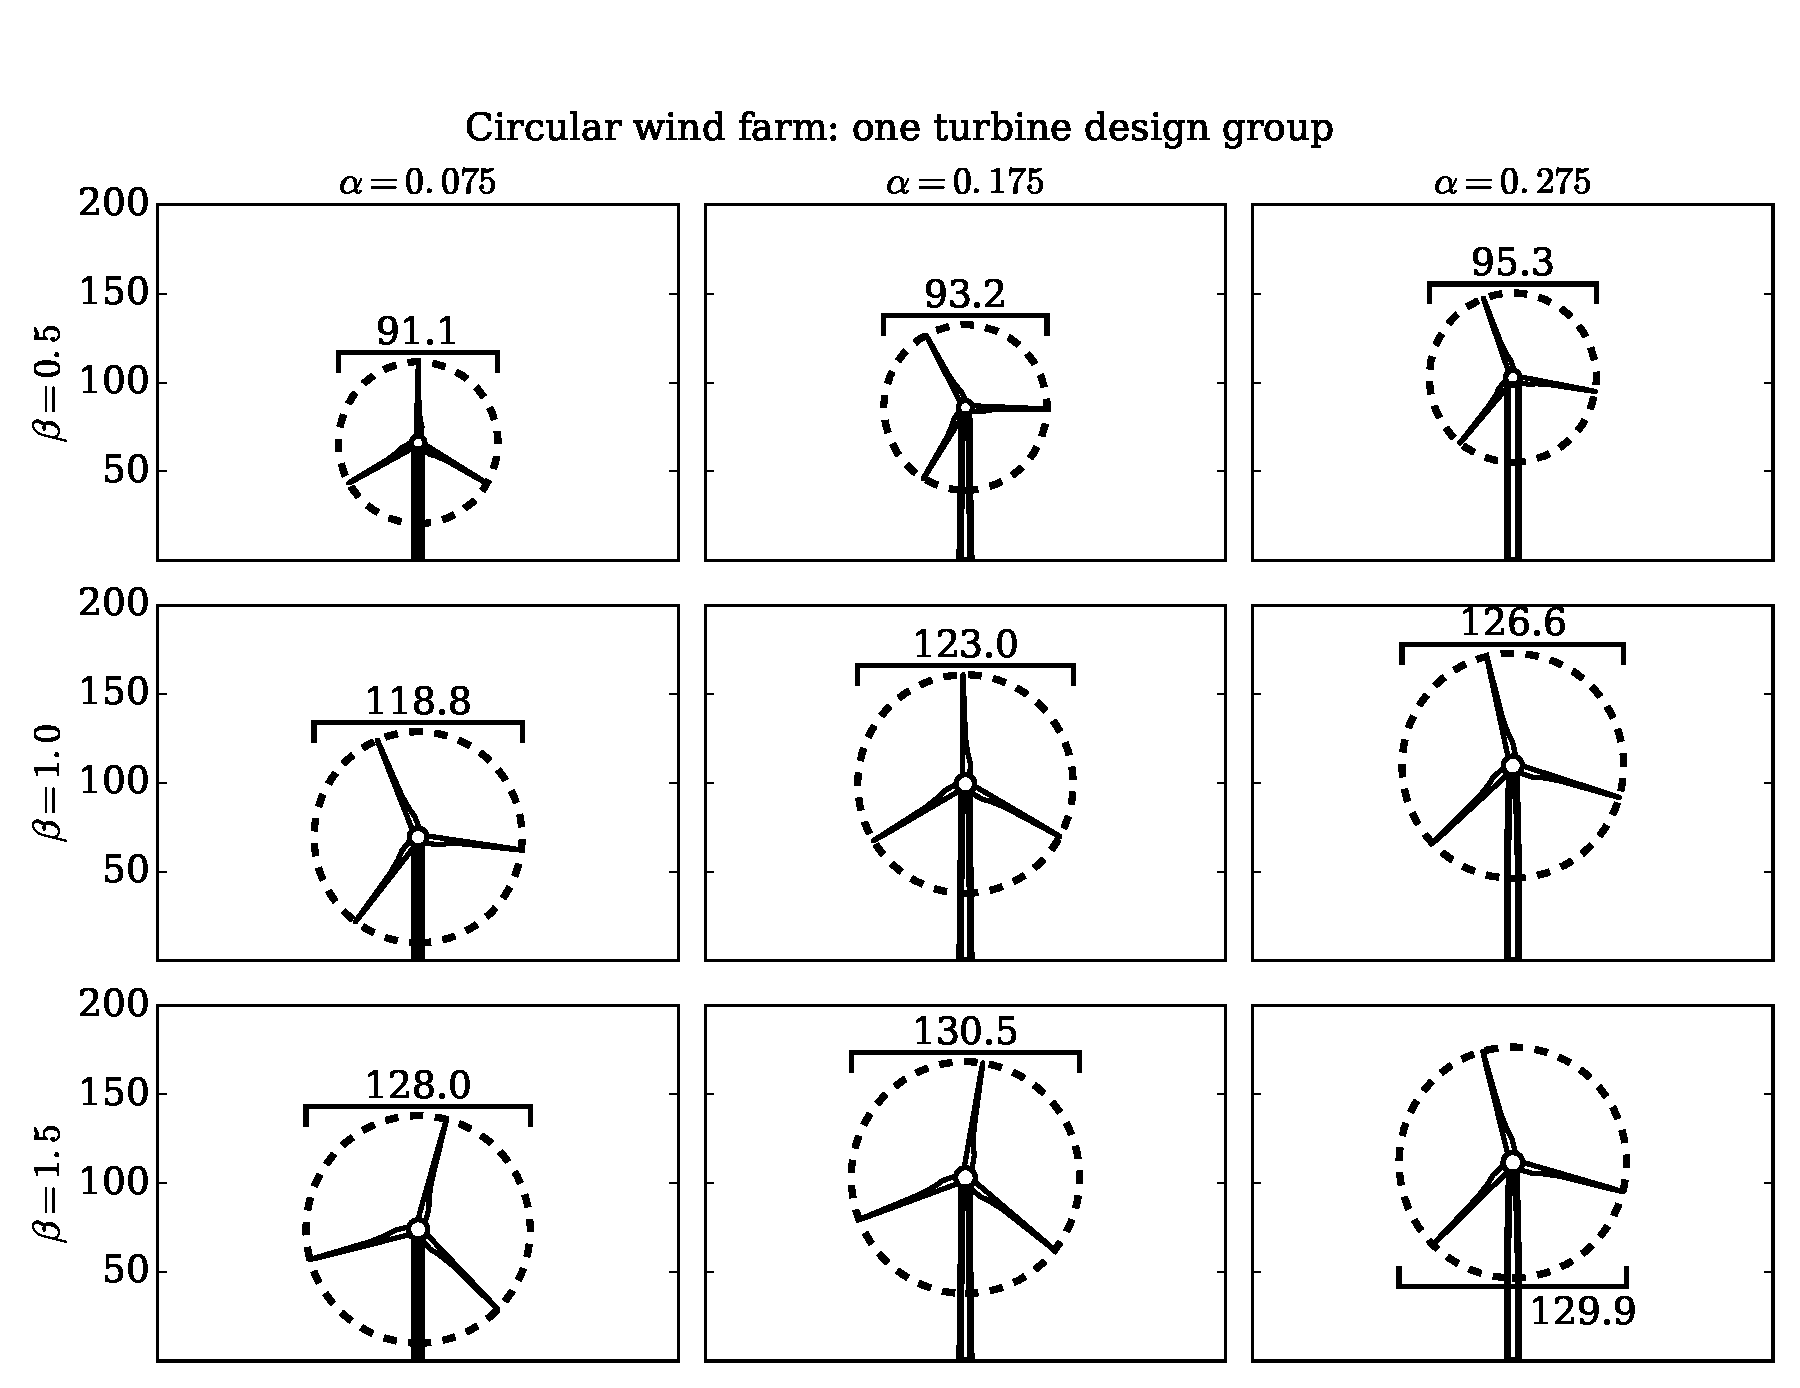
\includegraphics[trim={0.5cm 0.3cm 0.3cm 2.75cm},clip,width=0.7\textwidth]{Figures/turbineSizesCircular_1.pdf}
  \caption{\label{circular_turbines_1} The optimal turbine heights and rotor diameters for the optimization runs with coupled layout and turbine design with homogeneous turbine design throughout the circular wind farm. Each column shows a different shear exponent, with $\alpha=0.075,0.175,0.275$ from left to right. Each row shows a different farm spacing multiplier, with $\beta=0.5,1.0,1.5$ from top to bottom.}
\end{figure}


In Fig. \ref{circular_power}, the black points show the optimal rated powers for the turbines in each optimization case. Notice that the optimal rated power scales with the turbine rotor diameter and hub height. Higher turbine rating is expensive. Therefore, the small rotors and short turbines, which are more heavily waked and don't produce as much power, do not require a large power rating. The extra cost is not justified by a very slight increase in power. For the high shear exponents and spacing multipliers, the turbines are exposed to faster wind speeds. These turbines are bigger and taller, and the extra power production from raising the rated pwoer is worth the additional cost.


\begin{figure}[htbp]
  \centering
  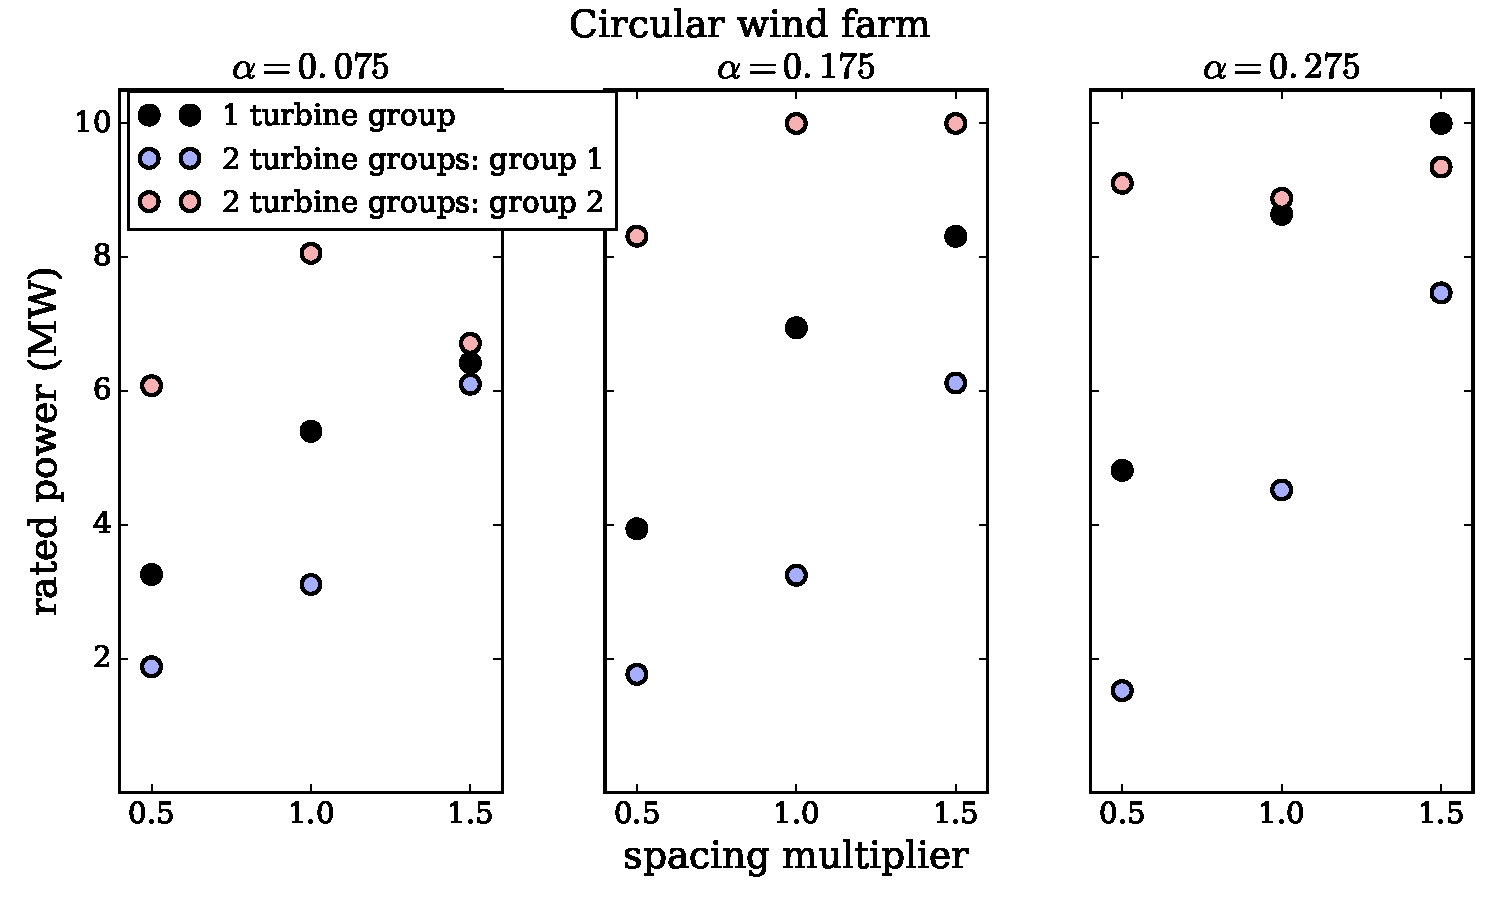
\includegraphics[trim={0.5cm 0.3cm 0.3cm 0.75cm},clip,width=0.7\textwidth]{Figures/circlePowers.pdf}
  \caption{\label{circular_power} The optimal rated powers for the circular wind farm for the optimization runs with coupled layout and turbine design for both uniform wind farm turbine design and with two different turbine design groups. The three subfigures show a different shear exponent, with $\alpha=0.075,0.175,0.275$ from left to right. within each subfigure, the x axis shows different farm spacing multipliers, with $\beta=0.5,1.0,1.5$ from left to right.}
\end{figure}



\subsubsection{Circular Wind Farm: Coupled Turbine Design and Layout Optimization with Two Turbine Groups}

Now we will discuss the most interesting case, the coupled turbine design and layout optimization with two different turbine groups. The optimal COE results of these optimziations are shown with the blue and pink points in Fig. \ref{circular_results}. Most visibly, for the smallest spacing multiplier, $\beta=0.5$, there is a large COE improvement for the hetergenous turbine design optimizations compared to the farms with homogeneous turbine design (shown by the black points in Fig. \ref{circular_results}). For this spacing multiplier, the heterogenous turbine design farms reduce COE by 21.6\%, 21.67\%, and 22.6\% compared to the layout-only optimization for shear exponents of $\alpha=0.075,0.175$, and $0.275$, respectively. The coupled optimizations with one turbine group reduce COE by 12.59\%, 10.24\%, and 11.15\%. For the smallest spacing multiplier, optimizing turbine design and layout with two turbine groups reduces COE by an additional 9--11.45\% compared to just one turbine group. For the spacing multiplier $\beta=1.0$, the coupled optimization with two turbine groups results in an additional 1.16--2.35\% COE decrease compared to with one turbine group. This is much smaller than the more tightly packed wind farms, but still non-negligible. For the spacing multiplier $\beta=1.5$, the optimization with two turbine groups results in only an additional 0--0.12\% COE decrease, indicating that when the turbines are spread very far apart there is no benefit to allowing multiple turbine designs in the same farm.

The two different rotor designs in the same wind farm help to improve COE by reducing the wake interaction between wind turbines. By combining tall and short turbines, with large and small rotor sizes, there are more dimensions that the optimizer can manipulate to avoid wakes and improve performance. For the tightly packed wind farms, the turbine layout is greatly limited by the turbine spacing constraints. Additionally, as the turbines are closer together, the wakes greatly reduce the wind speed as they have not had an opprtunity to mix with the freesteam air. Both of these factors mean there is a large benefit to avoiding the wakes of other turbines by any means possible. For the larger wind farms where the turbines are spaced farther apart, the wakes are not as detrimental and there is more area in which to avoid wakes in the horizontal plane without needing to change hub height or rotor diameter. In these cases, the heterogenous turbine designs are not as beneficial.

Figure \ref{circular_turbines} shows the optimal rotor diameter and hub height of each turbine group for these cases of coupled turbine design and layout optimization with two different groups. For the spacing multiplier $\beta=0.5$, when the turbines are very close together, there is a large difference in both the rotor diameter and hub height of each turbine group. Group 1 is extremely small and short, smaller than even the baseline rotor diameter, while group 2 is much larger. Even if turbines from each group were right next to each other, there would be minimal wake interaction between the turbines. For the small wind farms, the sacrifice in power that comes from one very small and short turbine is made up for in the decreased wake inteference between turbine groups. Essentially, having two different turbine groups doubles the effective spacing between turbines, because turbines in different groups do not affect each other. For a larger spacing multiplier of $\beta=1.0$, each turbine group is still remarkably different in size and height. The turbines are larger than they were for the smallest wind farm because the average wind speed is faster when the turbines are spread farther apart. Notice that, compared to the optimized turbines for $\beta=0.5$, the smaller turbines when $\beta=1.0$ are larger and overlap more with the taller, bigger turbines. In this case, the power increase from bigger rotor diameters outweighs the benefit gained from reducing wake interference. 

The turbine sizes for the largest wind farm, $\beta=1.5$, demonstrate the multi-modality of the wind farm optimization problem. For this spacing multiplier, each turbine group is more similar than in the previous wind farm sizes. For the lowest shear exponent, $\alpha=0.075$, both turbine groups are almost identical. For $\alpha=0.175,0.275$, there is some difference in each rotor diameter and hub height, although the difference is not as pronounced as it was for the smaller wind farms. However, Fig. \ref{circular_results} shows that for $\beta=1.5$ the optimal COE from coupled turbine design and layout optimization is the same with one and two height groups. So, a wind farm with the homogeneous turbine design shown in the bottom row of Fig. \ref{circular_turbines_1}, and a wind farm with two different turbine designs shown in the bottom row of Fig. \ref{circular_turbines} result in the same COE. The same optimal result is achieved with drastically different farms, each with different turbines and layouts.  

\begin{figure}[htbp]
  \centering
  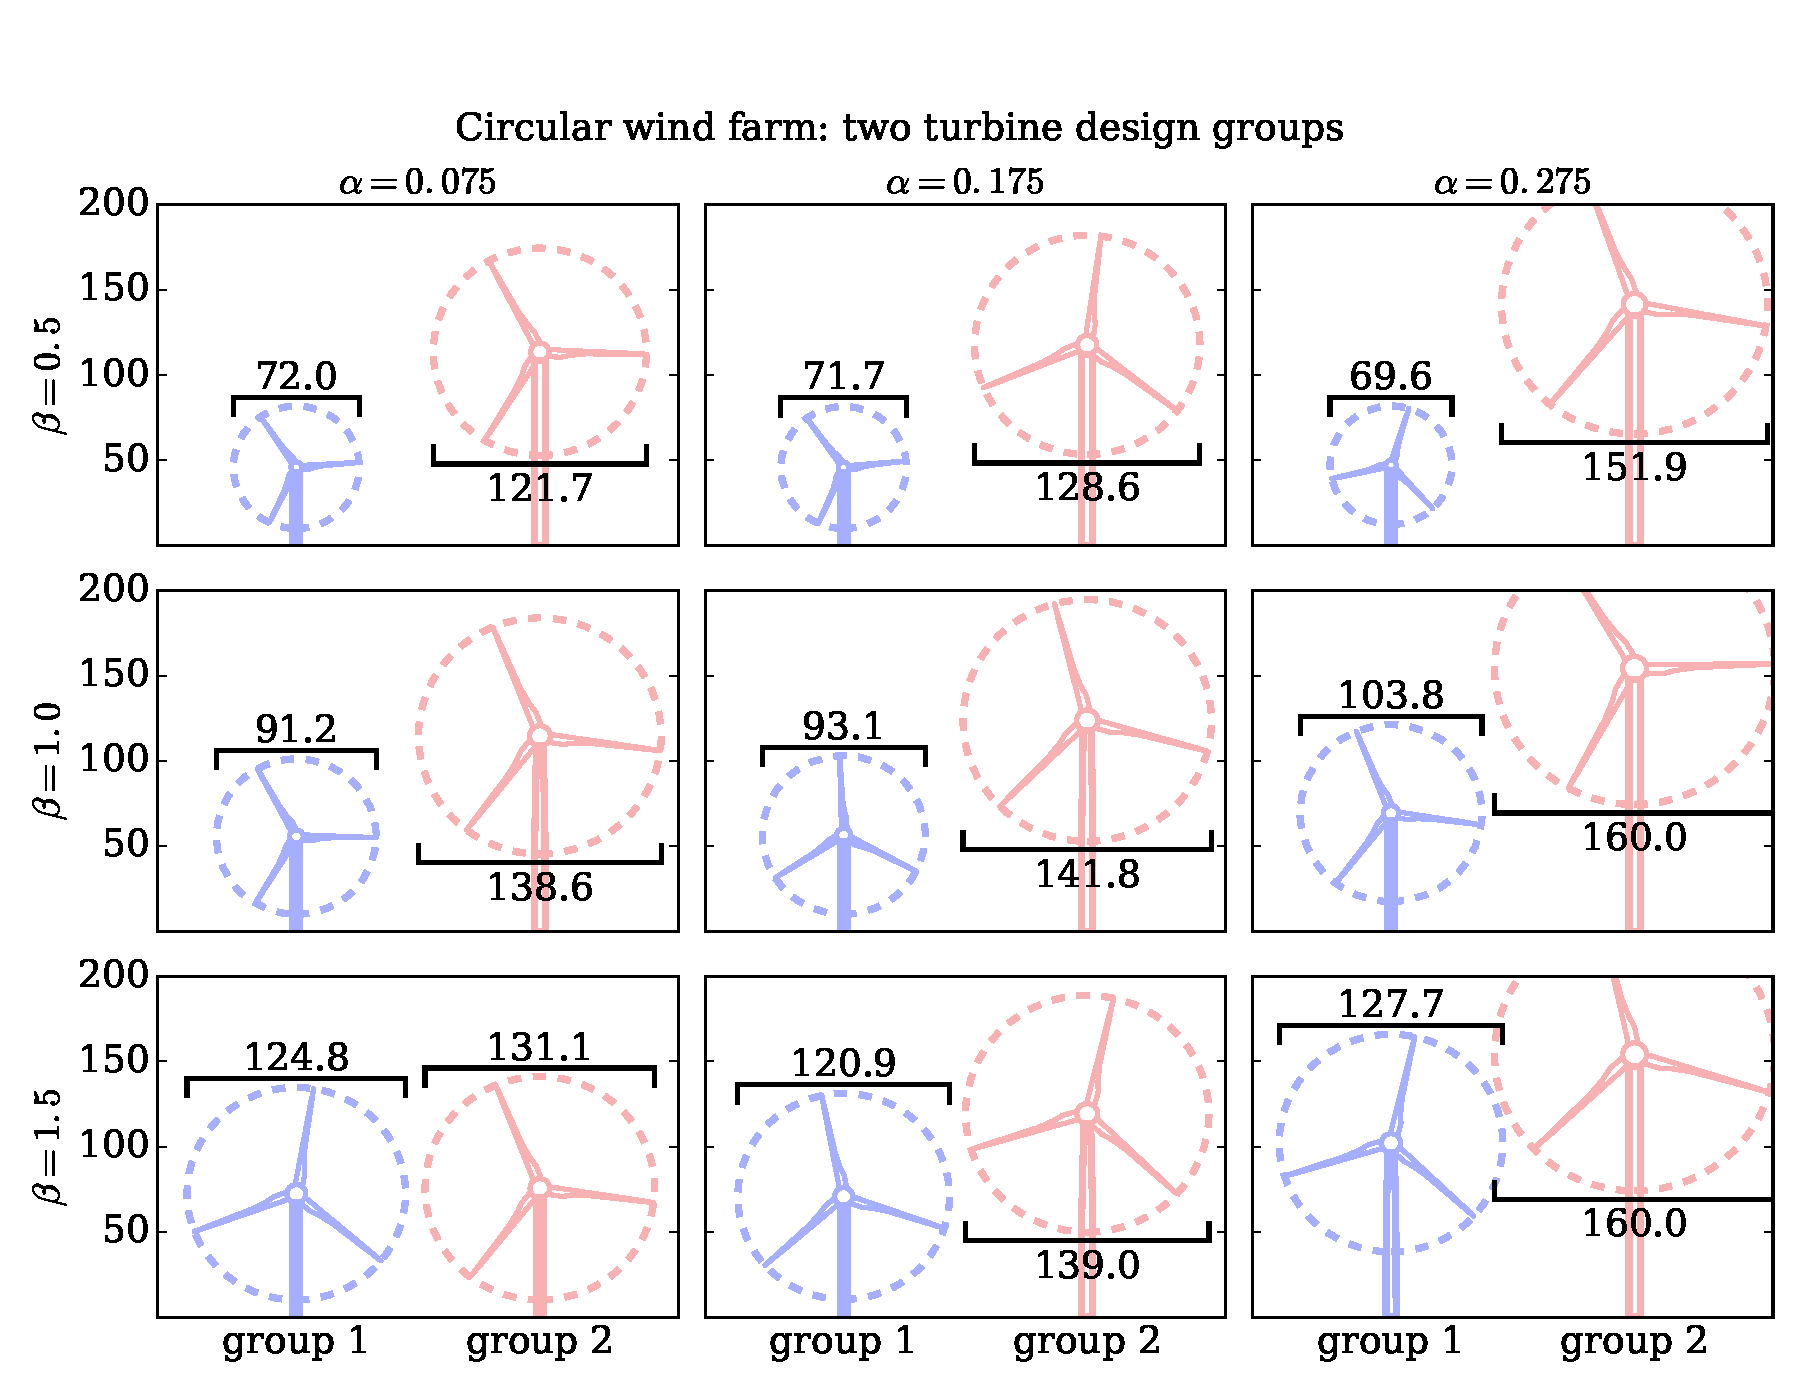
\includegraphics[trim={0.5cm 0.3cm 0.3cm 2.75cm},clip,width=0.7\textwidth]{Figures/turbineSizesCircular_2.pdf}
  \caption{\label{circular_turbines} The optimal turbine heights and rotor diameters for the optimization runs with coupled layout and turbine design with two different turbine design groups for the circular wind farm. Each column shows a different shear exponent, with $\alpha=0.075,0.175,0.275$ from left to right. Each row shows a different farm spacing multiplier, with $\beta=0.5,1.0,1.5$ from top to bottom.}
\end{figure}


Figure \ref{circular_power} shows the optimal rated power of each height group for the optimization cases with two different turbine groups. The blue and pink dots in this plot correspond to the turbines of the same color in Fig. \ref{circular_turbines}. As with the homogeneous turbine wind farm, the optimal rated power scales with the optimal turbine height and diameter. These larger, taller turbines are optimal in wind farms where they will be exposed to high wind speeds and produce large amounts of power. From a power production standpoint, it is undesirable to ever have a turbine's power limited by the rating. However, turbines with high ratings are more expensive, and not worth the cost if the turbine is generally producing low amounts of power. Therefore, the short, small turbines are optimal with a low, cheap power rating. The larger, taller turbines which produce much more electricity utilize the higher ratings.





\subsection{Princess Amalia Wind Farm Results}

Figure \ref{amalia_results} shows the COE results for the 60-turbine Princess Amalia wind farm optimizations.  The trends are similar to the smaller, circular wind farm. Coupled turbine design and layout optimization is superior to optimizing each sequentially, especially for the smaller wind farms where the wind speeds are much lower than the free stream. For the farms with closely spaced wind turbines, two different turbine designs in the same farm are significantly better than the farms optimized with a homogeneous turbine design. If the largest wind farms ($\beta=1.5$) benefit from two different turbine design groups, that benefit is negligible. The optimal COE values for the Princess Amalia wind farm are slightly lower across the board than the circular wind farm COE values. This is partly because there are more turbines in the Princess Amalia wind farm so a smaller portion of the total cost comes from overhead, but is partly due to the Princess Amalia wind turbines being spaced slightly farther apart than those in the circular wind farms. Another major difference between the optimal COE values of each wind farm is in the optimization case with two turbine design groups. For the Princess Amalia wind farm and a spacing multiplier of 0.5, two turbine groups provides and additional COE decrease of 6.13--9.11\% compared to the wind farm with homogeneous turbine design. This is significant, however it is not as large as the 9.01--11.45\% additional COE decrease in the circular wind farm optimizations for the same spacing multiplier. Again, the main cause of this seems to be that the circular wind farms are slightly closer together than the Princess Amalia wind farms.
The optimal turbine designs for the Princess Amalia wind farm optimizations were very similar to those for the circular wind farm, therefore will not be shown in this paper.




%Figures \ref{amalia_turbines_seq}, \ref{amalia_turbines_1},  and \ref{amalia_turbines} show the turbine rotor diameters and hub heights for the various optimization runs,  Fig. \ref{amalia_power} shows the optimal rated powers for the coupled turbine-design-and-layout optimizations, and Table \ref{amalia_table} tabulates the relative benefit of each optimization compared to the layout only optimization. The trends, and reasons behind them, are the same as for the circular wind farm optimizations. We will therefore not repeat this discussion, but will briefly discuss the significant differences between the optimizations of the 32-turbine circular wind farm and those for the 60-turbine Princess Amalia wind farm.  The conclusion remains the same, wind farms with closely spaced wind turbines greatly benefit from different turbine designs. The last significant difference between the wind farm is that the optimal turbine designs for the Princess Amalia wind farms are slightly smaller than in the circular wind farms. This is due to the different wind roses and speed distributions used to optimized each wind farm. 


\begin{figure}[htbp]
  \centering
  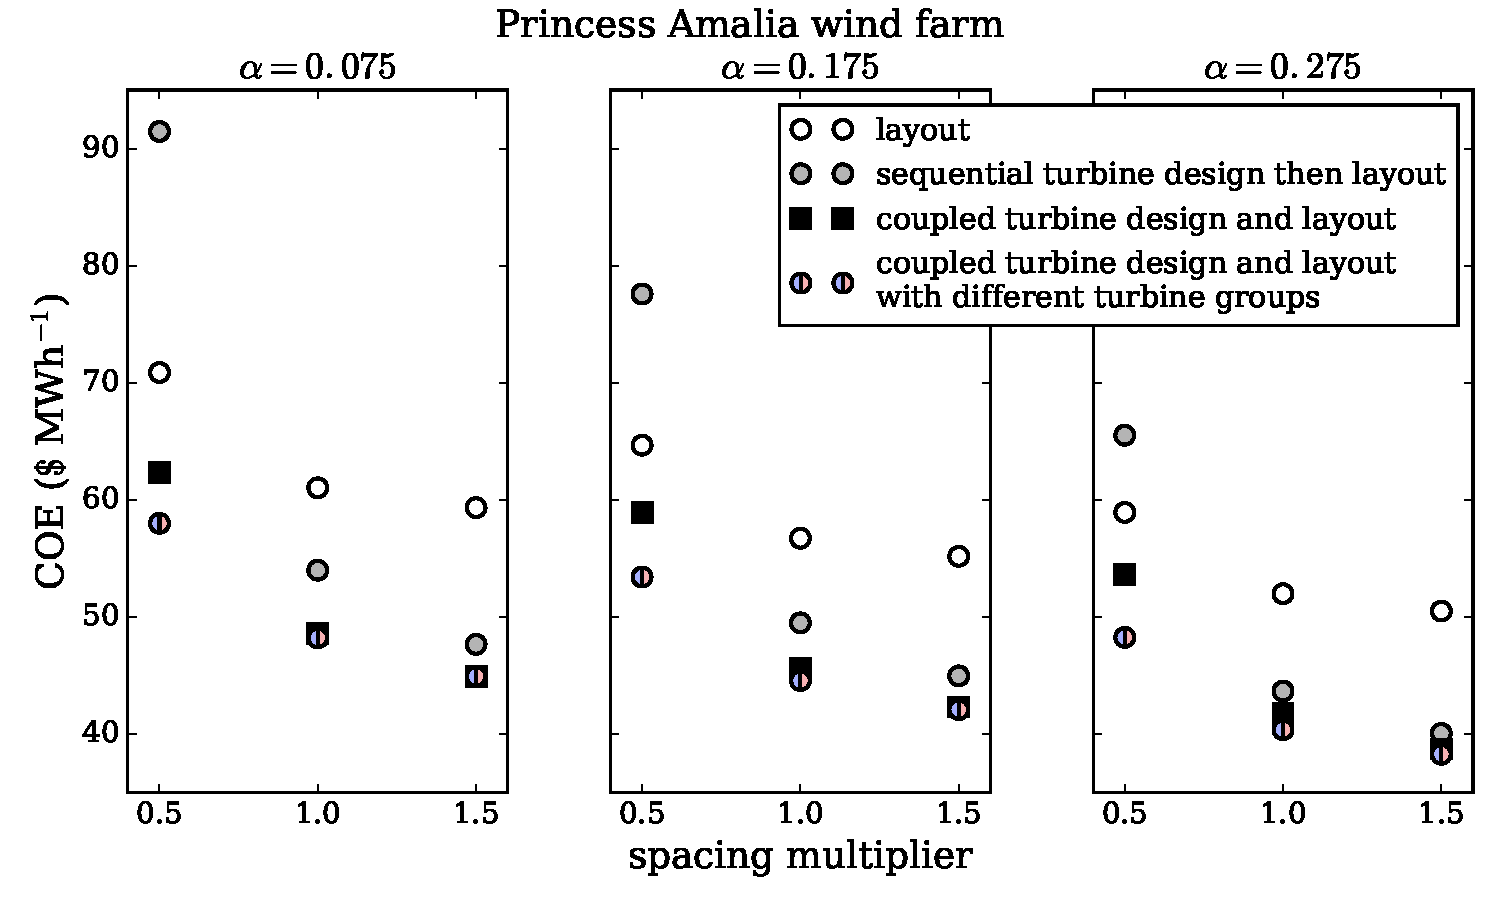
\includegraphics[width=0.7\textwidth]{Figures/amalia_results1.pdf}
  \caption{\label{amalia_results} The optimal COE results for the Princess Amalia wind farm layout with 32 turbines. Each of the subfigures corresponds to optimization runs with a different shear exponent, from left to right $\alpha=0.075,0.175,0.275$. Within each subfigure, the x axis shows the size of the wind farm based on the spacing multiplier, from left to right $\beta=0.5,1.0,1.5$. The different points represent the layout optimization, sequential turbine-design-then-layout optimization, coupled layout-and-turbine-design optimization with homogeneous turbine design throughout the farm, and layout-and-turbine-design optimization with two different turbine design groups.}
\end{figure}



Table \ref{results_table} shows how the optimal COE results for each wind farm compared to the layout optimization with the baseline wind turbine design. These numbers compare the relative benefit of performing turbine design with the various scenarios mentioned. High numbers represent a large COE decrease compared to the layout-only optimization for a given shear exponent and spacing multiplier combination, they do not necessarily represent a low COE.
There are a few interesting numbers in this table. Most obviously is the negative values (shown in red) for the sequential optimization with a spacing multiplier of 0.5. For these farms, sequential optimization is actually worse than the baseline. Also notice the COE decrease from coupled optimization with one group to two groups. For $\beta=0.5$, there is a huge benefit to having two groups, for $\beta=1.0$ there is a small benefit, and for $\beta=1.5$ there is no benefit at all. Finally, the benefit of coupled optimization with one group compared to sequential optimization is important. Again, there is a huge benefit to coupled optimization for the smallest spacing multiplier, and this relative benefit decreases as the wind farm size grows. However, even for $\beta=1.5$, there is an appreciable benefit to coupled design-and-layout optimization compared to sequential.
% Notice that for a spacing multiplier $\beta=0.5$, the relative improvement of two turbine design groups is far superior to coupled design and layout optimization with one turbine group. Also, for $\beta=0.5,1.0$, coupled turbine design and layout optimization is significantly better than the sequential optimization.




\begin{center}
\begin{table}
\caption{The percent COE decrease of the various optimization cases with respect to layout-only optimization. This table does not show the overall desirability of the optimal wind farm, but the relative improvement of different considerations of turbine design optimization. In the table are shown results for each shear exponent, $\alpha$, as well as each spacing multiplier, $\beta$, in which the smaller spacing multipliers represent farms with turbines that are more closely spaced.}
\label{results_table}
\begin{tabular}{p{2.5cm} c c c c c c c c c c c}
%\begin{tabularx}{\textwidth}{|X|c|c|c|c|c|c|c|c|c|}
\multicolumn{12}{c}{\textbf{Percent COE decrease compared to layout only optimization}}\\
\hline
\multicolumn{12}{c}{\textbf{circular wind farm}}\\
\hline
 & \multicolumn{3}{c}{$\alpha=0.075$} & \multicolumn{4}{c}{$\alpha=0.175$} & \multicolumn{4}{c}{$\alpha=0.275$}\\
\hline
optimization case & $\beta\myeq0.5$ & $\beta\myeq1.0$ & $\beta\myeq1.5$ & & $\beta\myeq0.5$ & $\beta\myeq1.0$ & $\beta\myeq1.5$& &$\beta\myeq0.5$ & $\beta\myeq1.0$ & $\beta\myeq1.5$\\
%\specialrule{.2em}{.1em}{.1em}
sequential & \textcolor{red}{-23.07} & 15.90 & 24.84 & & \textcolor{red}{-15.19}  & 18.13 & 24.37 & & \textcolor{red}{-6.97}  & 22.01 & 26.64\\
%\hline
coupled: 1 group& 12.59  & 22.72  & 27.62  & & 10.24  & 22.88  & 27.87 & & 11.15 & 24.66 & 28.52 \\
%\hline
coupled: 2 groups & 21.60  & 23.88  & 27.54 & & 21.67  & 25.23  &  27.90 & &  22.60 & 26.46  & 28.64\\
\hline


\multicolumn{12}{c}{\textbf{Princess Amalia wind farm}}\\
\hline
 & \multicolumn{3}{c}{$\alpha=0.075$} & \multicolumn{4}{c}{$\alpha=0.175$} & \multicolumn{4}{c}{$\alpha=0.275$}\\
\hline
optimization case & $\beta\myeq0.5$ & $\beta\myeq1.0$ & $\beta\myeq1.5$ & & $\beta\myeq0.5$ & $\beta\myeq1.0$ & $\beta\myeq1.5$& &$\beta\myeq0.5$ & $\beta\myeq1.0$ & $\beta\myeq1.5$\\
%\specialrule{.2em}{.1em}{.1em}
sequential & \textcolor{red}{-29.06} & 11.54 & 19.70 & & \textcolor{red}{-19.98}  & 12.74 & 18.52 & & \textcolor{red}{-11.19}  & 16.02 & 20.70\\
%\hline
coupled: 1 group& 12.05  & 20.45  & 24.34  & & 8.94  & 19.61  & 23.32 & & 9.00 & 19.66 & 23.33 \\
%\hline
coupled: 2 groups & 18.18  & 21.01  & 24.30 & & 17.41  & 21.45  &  23.74 & &  18.11 & 22.37  & 24.24\\
\hline
%\end{tabularx}
\end{tabular}
\end{table}
\end{center}












\conclusions  %% \conclusions[modified heading if necessary]
The purpose of this study was to optimize wind turbine design and turbine layout in various wind farms. There was a particular focus on benefits from coupled turbine design and layout optimization, as well as having different turbine designs in the same wind farm. We simulated wind farms in this study by modifying and combining a variety of separate wind farm models, including the FLORIS wake model, portions of TowerSE and Plant\_CostsSE, and a surrogate of RotorSE. Wind farms were optimized to minimize COE using turbine layout and turbine design including hub height, rotor diameter, rated power, and tower design, as design variables. We optimized two wind farms, a contrived 32-turbine circular wind farm, and the 60-turbine Princess Amalia wind farm. Both were optimized for a range of shear exponents and turbine spacings. 

Our main conclusions are twofold: coupled turbine design and layout optimization provides significant benefits compared to optimizing sequentially, and for many wind farms, two different turbine designs can greatly reduce the cost of energy. Without exception, coupled design and layout optimization performed better than optimizing the turbine design followed by the turbine layout. For a turbine design optimized in isolation, as was done in the sequential case, it was always most optimal to have a rotor diameter as large as the constraints would allow. Also, in coupled wind farm optimization, the wind farms with large spacing multipliers tended towards large rotor diameters. For this reason, the smallest wind farms benefited most from the coupled design and layout optimization, because the wind speeds were slow from strong wake interactions, and optimal rotor diameter was small---much different than the turbines optimized in isolation.

Including two different turbine designs in the same wind farm can be very beneficial in reducing wake interference between wind turbines and result in a lower COE compared to a farm with all identical wind turbines. For wind turbines that are close together, wake interactions are very strong between turbines. With different turbine sizes, the hub height and rotor diameter can be optimized along with layout to avoid wakes in the vertical plane along with the horizontal plane. For a spacing multiplier $\beta=0.5$, indicating very closely spaced wind turbines, our optimization results show that two different turbine designs can reduce COE by an additional 10\% compared to wind farms with homogeneous turbine design. For $\beta=1.0$, the farms with heterogeneous turbine designs are marginally better than the optimized farms with uniform design by 1--3\%. For the largest farms, $\beta=1.5$, there is no benefit to having two different turbine designs in the same wind farm. When the turbines are very far apart, the wake interactions are weak enough that the turbines can approach the turbine design optimized in isolation. 

%Our results indicate significantly superior wind farm designs when turbine design and layout are optimized as coupled design variables, and when two different turbine design groups are included in the same wind farm. Conservatively, this practice can reduce wind farm COE by 3--5\% for many wind farm spacings and wind shear conditions, and can reduce COE by upwards of 10\% for the more extreme cases.
% COE decrease when optimizing turbine design for the wind farm where it will operate. The original Princess Amalia wind farm (with $\beta=1.0$, so the original wind farm layout), experiences over a 20\% COE reduction when the wind turbines design is optimized along with the layout, for all wind shear exponents tested in this study. This is compared to the baseline wind farm, with 2 Megawatt turbines, 80 meter rotor diameter, and 100 meter hub height. 20\% COE decrease is unheard of! 
%According to the U.S. Energy Information Administration, onshore wind energy will have a similar COE as the projected cheapest energy sources, coal and natural gas, for new plants coming online in 2022 \citep{levelized}. Add onto this a 10\% COE reduction, and wind becomes by far the cheapest energy option available, even without any tax benefits. Coupling the optimization of turbine design and layout, and considering heterogeneous turbine design throughout a wind farm is the difference between a clean, cheap energy source, and the cheapest energy source regardless of any other consideration. 




%% The following commands are for the statements about the availability of data sets and/or software code corresponding to the manuscript.
%% It is strongly recommended to make use of these sections in case data sets and/or software code have been part of your research the article is based on.

%\codeavailability{TEXT} %% use this section when having only software code available


%\dataavailability{TEXT} %% use this section when having only data sets available


\codedataavailability{TEXT} %% use this section when having data sets and software code available


%\sampleavailability{TEXT} %% use this section when having geoscientific samples available



%\appendix
%\section{}    %% Appendix A

%\subsection{}     %% Appendix A1, A2, etc.


%\noappendix       %% use this to mark the end of the appendix section

%% Regarding figures and tables in appendices, the following two options are possible depending on your general handling of figures and tables in the manuscript environment:

%% Option 1: If you sorted all figures and tables into the sections of the text, please also sort the appendix figures and appendix tables into the respective appendix sections.
%% They will be correctly named automatically.

%% Option 2: If you put all figures after the reference list, please insert appendix tables and figures after the normal tables and figures.
%% To rename them correctly to A1, A2, etc., please add the following commands in front of them:

%\appendixfigures  %% needs to be added in front of appendix figures

%\appendixtables   %% needs to be added in front of appendix tables

%% Please add \clearpage between each table and/or figure. Further guidelines on figures and tables can be found below.



%\authorcontribution{TEXT} %% optional section

\competinginterests{The authors declare that they have no conflict of interest.} %% this section is mandatory even if you declare that no competing interests are present

%\disclaimer{TEXT} %% optional section

\begin{acknowledgements}
The authors developed this journal article based on funding from the Alliance for Sustainable Energy, LLC, Managing and Operating Contractor for the National Renewable Energy Laboratory for the U.S. Department of Energy. 

Funding for the work was provided by the DOE Office of Energy Efficiency and Renewable Energy, Wind Energy Technologies Office.

The U.S. Government retains and the publisher, by accepting the article for publication, acknowledges that the U.S. Government retains a nonexclusive, paid-up, irrevocable, worldwide license to publish or reproduce the published form of this work, or allow others to do so, for U.S. Government purposes.
\end{acknowledgements}




%% REFERENCES

%% The reference list is compiled as follows:


%% Since the Copernicus LaTeX package includes the BibTeX style file copernicus.bst,
%% authors experienced with BibTeX only have to include the following two lines:
%%
\bibliographystyle{copernicus}
\bibliography{references.bib}
%%
%% URLs and DOIs can be entered in your BibTeX file as:
%%
%% URL = {http://www.xyz.org/~jones/idx_g.htm}
%% DOI = {10.5194/xyz}


%% LITERATURE CITATIONS
%%
%% command                        & example result
%% \citet{jones90}|               & Jones et al. (1990)
%% \citep{jones90}|               & (Jones et al., 1990)
%% \citep{jones90,jones93}|       & (Jones et al., 1990, 1993)
%% \citep[p.~32]{jones90}|        & (Jones et al., 1990, p.~32)
%% \citep[e.g.,][]{jones90}|      & (e.g., Jones et al., 1990)
%% \citep[e.g.,][p.~32]{jones90}| & (e.g., Jones et al., 1990, p.~32)
%% \citeauthor{jones90}|          & Jones et al.
%% \citeyear{jones90}|            & 1990



%% FIGURES

%% When figures and tables are placed at the end of the MS (article in one-column style), please add \clearpage
%% between bibliography and first table and/or figure as well as between each table and/or figure.


%% ONE-COLUMN FIGURES

%%f
%\begin{figure}[t]
%\includegraphics[width=8.3cm]{FILE NAME}
%\caption{TEXT}
%\end{figure}
%
%%% TWO-COLUMN FIGURES
%
%%f
%\begin{figure*}[t]
%\includegraphics[width=12cm]{FILE NAME}
%\caption{TEXT}
%\end{figure*}
%
%
%%% TABLES
%%%
%%% The different columns must be seperated with a & command and should
%%% end with \\ to identify the column brake.
%
%%% ONE-COLUMN TABLE
%
%%t
%\begin{table}[t]
%\caption{TEXT}
%\begin{tabular}{column = lcr}
%\tophline
%
%\middlehline
%
%\bottomhline
%\end{tabular}
%\belowtable{} % Table Footnotes
%\end{table}
%
%%% TWO-COLUMN TABLE
%
%%t
%\begin{table*}[t]
%\caption{TEXT}
%\begin{tabular}{column = lcr}
%\tophline
%
%\middlehline
%
%\bottomhline
%\end{tabular}
%\belowtable{} % Table Footnotes
%\end{table*}
%
%%% LANDSCAPE TABLE
%
%%t
%\begin{sidewaystable*}[t]
%\caption{TEXT}
%\begin{tabular}{column = lcr}
%\tophline
%
%\middlehline
%
%\bottomhline
%\end{tabular}
%\belowtable{} % Table Footnotes
%\end{sidewaystable*}
%
%
%%% MATHEMATICAL EXPRESSIONS
%
%%% All papers typeset by Copernicus Publications follow the math typesetting regulations
%%% given by the IUPAC Green Book (IUPAC: Quantities, Units and Symbols in Physical Chemistry,
%%% 2nd Edn., Blackwell Science, available at: http://old.iupac.org/publications/books/gbook/green_book_2ed.pdf, 1993).
%%%
%%% Physical quantities/variables are typeset in italic font (t for time, T for Temperature)
%%% Indices which are not defined are typeset in italic font (x, y, z, a, b, c)
%%% Items/objects which are defined are typeset in roman font (Car A, Car B)
%%% Descriptions/specifications which are defined by itself are typeset in roman font (abs, rel, ref, tot, net, ice)
%%% Abbreviations from 2 letters are typeset in roman font (RH, LAI)
%%% Vectors are identified in bold italic font using \vec{x}
%%% Matrices are identified in bold roman font
%%% Multiplication signs are typeset using the LaTeX commands \times (for vector products, grids, and exponential notations) or \cdot
%%% The character * should not be applied as mutliplication sign
%
%
%%% EQUATIONS
%
%%% Single-row equation
%
%\begin{equation}
%
%\end{equation}
%
%%% Multiline equation
%
%\begin{align}
%& 3 + 5 = 8\\
%& 3 + 5 = 8\\
%& 3 + 5 = 8
%\end{align}
%
%
%%% MATRICES
%
%\begin{matrix}
%x & y & z\\
%x & y & z\\
%x & y & z\\
%\end{matrix}
%
%
%%% ALGORITHM
%
%\begin{algorithm}
%\caption{...}
%\label{a1}
%\begin{algorithmic}
%...
%\end{algorithmic}
%\end{algorithm}
%
%
%%% CHEMICAL FORMULAS AND REACTIONS
%
%%% For formulas embedded in the text, please use \chem{}
%
%%% The reaction environment creates labels including the letter R, i.e. (R1), (R2), etc.
%
%\begin{reaction}
%%% \rightarrow should be used for normal (one-way) chemical reactions
%%% \rightleftharpoons should be used for equilibria
%%% \leftrightarrow should be used for resonance structures
%\end{reaction}
%
%
%%% PHYSICAL UNITS
%%%
%%% Please use \unit{} and apply the exponential notation


\end{document}
